\documentclass[twoside]{book}

% Packages required by doxygen
\usepackage{fixltx2e}
\usepackage{calc}
\usepackage{doxygen}
\usepackage[export]{adjustbox} % also loads graphicx
\usepackage{graphicx}
\usepackage[utf8]{inputenc}
\usepackage{makeidx}
\usepackage{multicol}
\usepackage{multirow}
\PassOptionsToPackage{warn}{textcomp}
\usepackage{textcomp}
\usepackage[nointegrals]{wasysym}
\usepackage[table]{xcolor}

% Font selection
\usepackage[T1]{fontenc}
\usepackage[scaled=.90]{helvet}
\usepackage{courier}
\usepackage{amssymb}
\usepackage{sectsty}
\renewcommand{\familydefault}{\sfdefault}
\allsectionsfont{%
  \fontseries{bc}\selectfont%
  \color{darkgray}%
}
\renewcommand{\DoxyLabelFont}{%
  \fontseries{bc}\selectfont%
  \color{darkgray}%
}
\newcommand{\+}{\discretionary{\mbox{\scriptsize$\hookleftarrow$}}{}{}}

% Page & text layout
\usepackage{geometry}
\geometry{%
  a4paper,%
  top=2.5cm,%
  bottom=2.5cm,%
  left=2.5cm,%
  right=2.5cm%
}
\tolerance=750
\hfuzz=15pt
\hbadness=750
\setlength{\emergencystretch}{15pt}
\setlength{\parindent}{0cm}
\setlength{\parskip}{3ex plus 2ex minus 2ex}
\makeatletter
\renewcommand{\paragraph}{%
  \@startsection{paragraph}{4}{0ex}{-1.0ex}{1.0ex}{%
    \normalfont\normalsize\bfseries\SS@parafont%
  }%
}
\renewcommand{\subparagraph}{%
  \@startsection{subparagraph}{5}{0ex}{-1.0ex}{1.0ex}{%
    \normalfont\normalsize\bfseries\SS@subparafont%
  }%
}
\makeatother

% Headers & footers
\usepackage{fancyhdr}
\pagestyle{fancyplain}
\fancyhead[LE]{\fancyplain{}{\bfseries\thepage}}
\fancyhead[CE]{\fancyplain{}{}}
\fancyhead[RE]{\fancyplain{}{\bfseries\leftmark}}
\fancyhead[LO]{\fancyplain{}{\bfseries\rightmark}}
\fancyhead[CO]{\fancyplain{}{}}
\fancyhead[RO]{\fancyplain{}{\bfseries\thepage}}
\fancyfoot[LE]{\fancyplain{}{}}
\fancyfoot[CE]{\fancyplain{}{}}
\fancyfoot[RE]{\fancyplain{}{\bfseries\scriptsize Generated by Doxygen }}
\fancyfoot[LO]{\fancyplain{}{\bfseries\scriptsize Generated by Doxygen }}
\fancyfoot[CO]{\fancyplain{}{}}
\fancyfoot[RO]{\fancyplain{}{}}
\renewcommand{\footrulewidth}{0.4pt}
\renewcommand{\chaptermark}[1]{%
  \markboth{#1}{}%
}
\renewcommand{\sectionmark}[1]{%
  \markright{\thesection\ #1}%
}

% Indices & bibliography
\usepackage{natbib}
\usepackage[titles]{tocloft}
\setcounter{tocdepth}{3}
\setcounter{secnumdepth}{5}
\makeindex

% Hyperlinks (required, but should be loaded last)
\usepackage{ifpdf}
\ifpdf
  \usepackage[pdftex,pagebackref=true]{hyperref}
\else
  \usepackage[ps2pdf,pagebackref=true]{hyperref}
\fi
\hypersetup{%
  colorlinks=true,%
  linkcolor=blue,%
  citecolor=blue,%
  unicode%
}

% Custom commands
\newcommand{\clearemptydoublepage}{%
  \newpage{\pagestyle{empty}\cleardoublepage}%
}

\usepackage{caption}
\captionsetup{labelsep=space,justification=centering,font={bf},singlelinecheck=off,skip=4pt,position=top}

%===== C O N T E N T S =====

\begin{document}

% Titlepage & ToC
\hypersetup{pageanchor=false,
             bookmarksnumbered=true,
             pdfencoding=unicode
            }
\pagenumbering{alph}
\begin{titlepage}
\vspace*{7cm}
\begin{center}%
{\Large bluecloud.\+extensions \\[1ex]\large 1.\+0.\+2 }\\
\vspace*{1cm}
{\large Generated by Doxygen 1.8.14}\\
\end{center}
\end{titlepage}
\clearemptydoublepage
\pagenumbering{roman}
\tableofcontents
\clearemptydoublepage
\pagenumbering{arabic}
\hypersetup{pageanchor=true}

%--- Begin generated contents ---
\chapter{Namespace Index}
\section{Namespace List}
Here is a list of all documented namespaces with brief descriptions\+:\begin{DoxyCompactList}
\item\contentsline{section}{\mbox{\hyperlink{namespace_blue_cloud}{Blue\+Cloud}} }{\pageref{namespace_blue_cloud}}{}
\item\contentsline{section}{\mbox{\hyperlink{namespace_blue_cloud_1_1_extensions}{Blue\+Cloud.\+Extensions}} }{\pageref{namespace_blue_cloud_1_1_extensions}}{}
\item\contentsline{section}{\mbox{\hyperlink{namespace_blue_cloud_1_1_extensions_1_1_assembly}{Blue\+Cloud.\+Extensions.\+Assembly}} }{\pageref{namespace_blue_cloud_1_1_extensions_1_1_assembly}}{}
\item\contentsline{section}{\mbox{\hyperlink{namespace_blue_cloud_1_1_extensions_1_1_cache}{Blue\+Cloud.\+Extensions.\+Cache}} }{\pageref{namespace_blue_cloud_1_1_extensions_1_1_cache}}{}
\item\contentsline{section}{\mbox{\hyperlink{namespace_blue_cloud_1_1_extensions_1_1_collections}{Blue\+Cloud.\+Extensions.\+Collections}} }{\pageref{namespace_blue_cloud_1_1_extensions_1_1_collections}}{}
\item\contentsline{section}{\mbox{\hyperlink{namespace_blue_cloud_1_1_extensions_1_1_data}{Blue\+Cloud.\+Extensions.\+Data}} }{\pageref{namespace_blue_cloud_1_1_extensions_1_1_data}}{}
\item\contentsline{section}{\mbox{\hyperlink{namespace_blue_cloud_1_1_extensions_1_1_string}{Blue\+Cloud.\+Extensions.\+String}} }{\pageref{namespace_blue_cloud_1_1_extensions_1_1_string}}{}
\end{DoxyCompactList}

\chapter{Hierarchical Index}
\section{Class Hierarchy}
This inheritance list is sorted roughly, but not completely, alphabetically\+:\begin{DoxyCompactList}
\item \contentsline{section}{Blue\+Cloud.\+Extensions.\+Assembly.\+Assembly\+Extensions}{\pageref{class_blue_cloud_1_1_extensions_1_1_assembly_1_1_assembly_extensions}}{}
\item Attribute\begin{DoxyCompactList}
\item \contentsline{section}{Blue\+Cloud.\+Extensions.\+Data.\+Db\+Field\+Attribute}{\pageref{class_blue_cloud_1_1_extensions_1_1_data_1_1_db_field_attribute}}{}
\end{DoxyCompactList}
\item \contentsline{section}{Blue\+Cloud.\+Extensions.\+Data.\+Db\+Mapping}{\pageref{class_blue_cloud_1_1_extensions_1_1_data_1_1_db_mapping}}{}
\item \contentsline{section}{Blue\+Cloud.\+Extensions.\+Cache.\+I\+Cacheable$<$ T $>$}{\pageref{interface_blue_cloud_1_1_extensions_1_1_cache_1_1_i_cacheable}}{}
\begin{DoxyCompactList}
\item \contentsline{section}{Blue\+Cloud.\+Extensions.\+Cache.\+Default\+Cache$<$ T $>$}{\pageref{class_blue_cloud_1_1_extensions_1_1_cache_1_1_default_cache}}{}
\end{DoxyCompactList}
\item \contentsline{section}{Blue\+Cloud.\+Extensions.\+Cache.\+I\+Cacheable$<$ List$<$ Blue\+Cloud.\+Extensions.\+Data.\+Db\+Mapping $>$ $>$}{\pageref{interface_blue_cloud_1_1_extensions_1_1_cache_1_1_i_cacheable}}{}
\item \contentsline{section}{Blue\+Cloud.\+Extensions.\+Data.\+I\+Data\+Reader\+Extensions}{\pageref{class_blue_cloud_1_1_extensions_1_1_data_1_1_i_data_reader_extensions}}{}
\item \contentsline{section}{Blue\+Cloud.\+Extensions.\+Data.\+I\+Db\+Command\+Extensions}{\pageref{class_blue_cloud_1_1_extensions_1_1_data_1_1_i_db_command_extensions}}{}
\item \contentsline{section}{Blue\+Cloud.\+Extensions.\+Data.\+I\+Db\+Connection\+Extensions}{\pageref{class_blue_cloud_1_1_extensions_1_1_data_1_1_i_db_connection_extensions}}{}
\item \contentsline{section}{Blue\+Cloud.\+Extensions.\+Data.\+I\+Db\+Hydration\+Overridable}{\pageref{interface_blue_cloud_1_1_extensions_1_1_data_1_1_i_db_hydration_overridable}}{}
\item \contentsline{section}{Blue\+Cloud.\+Extensions.\+Data.\+I\+Db\+Serialization\+Overridable}{\pageref{interface_blue_cloud_1_1_extensions_1_1_data_1_1_i_db_serialization_overridable}}{}
\item I\+Disposable\begin{DoxyCompactList}
\item \contentsline{section}{Blue\+Cloud.\+Extensions.\+Cache.\+Default\+Cache$<$ T $>$}{\pageref{class_blue_cloud_1_1_extensions_1_1_cache_1_1_default_cache}}{}
\end{DoxyCompactList}
\item \contentsline{section}{Blue\+Cloud.\+Extensions.\+Collections.\+I\+Enumerable\+Extensions}{\pageref{class_blue_cloud_1_1_extensions_1_1_collections_1_1_i_enumerable_extensions}}{}
\item \contentsline{section}{Blue\+Cloud.\+Extensions.\+Collections.\+Match\+Collection\+Extensions}{\pageref{class_blue_cloud_1_1_extensions_1_1_collections_1_1_match_collection_extensions}}{}
\item \contentsline{section}{Blue\+Cloud.\+Extensions.\+String.\+String\+Extensions}{\pageref{class_blue_cloud_1_1_extensions_1_1_string_1_1_string_extensions}}{}
\end{DoxyCompactList}

\chapter{Class Index}
\section{Class List}
Here are the classes, structs, unions and interfaces with brief descriptions\+:\begin{DoxyCompactList}
\item\contentsline{section}{\mbox{\hyperlink{class_blue_cloud_1_1_extensions_1_1_assembly_1_1_assembly_extensions}{Blue\+Cloud.\+Extensions.\+Assembly.\+Assembly\+Extensions}} \\*Extension Methods for System.\+Reflection.\+Assembly }{\pageref{class_blue_cloud_1_1_extensions_1_1_assembly_1_1_assembly_extensions}}{}
\item\contentsline{section}{\mbox{\hyperlink{class_blue_cloud_1_1_extensions_1_1_data_1_1_db_field_attribute}{Blue\+Cloud.\+Extensions.\+Data.\+Db\+Field\+Attribute}} \\*Db\+Field Attribute used to annotate properties to be mapped to database fields. }{\pageref{class_blue_cloud_1_1_extensions_1_1_data_1_1_db_field_attribute}}{}
\item\contentsline{section}{\mbox{\hyperlink{class_blue_cloud_1_1_extensions_1_1_data_1_1_db_mapping}{Blue\+Cloud.\+Extensions.\+Data.\+Db\+Mapping}} \\*Db mapping. }{\pageref{class_blue_cloud_1_1_extensions_1_1_data_1_1_db_mapping}}{}
\item\contentsline{section}{\mbox{\hyperlink{class_blue_cloud_1_1_extensions_1_1_cache_1_1_default_cache}{Blue\+Cloud.\+Extensions.\+Cache.\+Default\+Cache$<$ T $>$}} \\*Default cache utilizing System.\+Runtime.\+Caching.\+Memory\+Cache }{\pageref{class_blue_cloud_1_1_extensions_1_1_cache_1_1_default_cache}}{}
\item\contentsline{section}{\mbox{\hyperlink{interface_blue_cloud_1_1_extensions_1_1_cache_1_1_i_cacheable}{Blue\+Cloud.\+Extensions.\+Cache.\+I\+Cacheable$<$ T $>$}} \\*\mbox{\hyperlink{interface_blue_cloud_1_1_extensions_1_1_cache_1_1_i_cacheable}{I\+Cacheable}} Interface used for caching database field to object property mappings. Customize caching with your own implementation. }{\pageref{interface_blue_cloud_1_1_extensions_1_1_cache_1_1_i_cacheable}}{}
\item\contentsline{section}{\mbox{\hyperlink{class_blue_cloud_1_1_extensions_1_1_data_1_1_i_data_reader_extensions}{Blue\+Cloud.\+Extensions.\+Data.\+I\+Data\+Reader\+Extensions}} \\*Extension Methods for System.\+Data.\+I\+Data\+Reader }{\pageref{class_blue_cloud_1_1_extensions_1_1_data_1_1_i_data_reader_extensions}}{}
\item\contentsline{section}{\mbox{\hyperlink{class_blue_cloud_1_1_extensions_1_1_data_1_1_i_db_command_extensions}{Blue\+Cloud.\+Extensions.\+Data.\+I\+Db\+Command\+Extensions}} \\*Extension Methods for System.\+Data.\+I\+Db\+Command }{\pageref{class_blue_cloud_1_1_extensions_1_1_data_1_1_i_db_command_extensions}}{}
\item\contentsline{section}{\mbox{\hyperlink{class_blue_cloud_1_1_extensions_1_1_data_1_1_i_db_connection_extensions}{Blue\+Cloud.\+Extensions.\+Data.\+I\+Db\+Connection\+Extensions}} \\*Extension Methods for System.\+Data.\+I\+Db\+Connection }{\pageref{class_blue_cloud_1_1_extensions_1_1_data_1_1_i_db_connection_extensions}}{}
\item\contentsline{section}{\mbox{\hyperlink{interface_blue_cloud_1_1_extensions_1_1_data_1_1_i_db_hydration_overridable}{Blue\+Cloud.\+Extensions.\+Data.\+I\+Db\+Hydration\+Overridable}} \\*\mbox{\hyperlink{interface_blue_cloud_1_1_extensions_1_1_data_1_1_i_db_hydration_overridable}{I\+Db\+Hydration\+Overridable}} used to customize property hydration. }{\pageref{interface_blue_cloud_1_1_extensions_1_1_data_1_1_i_db_hydration_overridable}}{}
\item\contentsline{section}{\mbox{\hyperlink{interface_blue_cloud_1_1_extensions_1_1_data_1_1_i_db_serialization_overridable}{Blue\+Cloud.\+Extensions.\+Data.\+I\+Db\+Serialization\+Overridable}} \\*\mbox{\hyperlink{interface_blue_cloud_1_1_extensions_1_1_data_1_1_i_db_serialization_overridable}{I\+Db\+Serialization\+Overridable}} used to customize property database serialization. }{\pageref{interface_blue_cloud_1_1_extensions_1_1_data_1_1_i_db_serialization_overridable}}{}
\item\contentsline{section}{\mbox{\hyperlink{class_blue_cloud_1_1_extensions_1_1_collections_1_1_i_enumerable_extensions}{Blue\+Cloud.\+Extensions.\+Collections.\+I\+Enumerable\+Extensions}} \\*Extension Methods for the I\+Enumerable Interface. }{\pageref{class_blue_cloud_1_1_extensions_1_1_collections_1_1_i_enumerable_extensions}}{}
\item\contentsline{section}{\mbox{\hyperlink{class_blue_cloud_1_1_extensions_1_1_collections_1_1_match_collection_extensions}{Blue\+Cloud.\+Extensions.\+Collections.\+Match\+Collection\+Extensions}} \\*Extension Methods for System.\+Text.\+Regular\+Expressions.\+Match\+Collection }{\pageref{class_blue_cloud_1_1_extensions_1_1_collections_1_1_match_collection_extensions}}{}
\item\contentsline{section}{\mbox{\hyperlink{class_blue_cloud_1_1_extensions_1_1_string_1_1_string_extensions}{Blue\+Cloud.\+Extensions.\+String.\+String\+Extensions}} \\*Extension Methods for System.\+String }{\pageref{class_blue_cloud_1_1_extensions_1_1_string_1_1_string_extensions}}{}
\end{DoxyCompactList}

\chapter{Namespace Documentation}
\hypertarget{namespace_blue_cloud}{}\section{Blue\+Cloud Namespace Reference}
\label{namespace_blue_cloud}\index{Blue\+Cloud@{Blue\+Cloud}}
\subsection*{Namespaces}
\begin{DoxyCompactItemize}
\end{DoxyCompactItemize}

\hypertarget{namespace_blue_cloud_1_1_extensions}{}\section{Blue\+Cloud.\+Extensions Namespace Reference}
\label{namespace_blue_cloud_1_1_extensions}\index{Blue\+Cloud.\+Extensions@{Blue\+Cloud.\+Extensions}}
\subsection*{Namespaces}
\begin{DoxyCompactItemize}
\end{DoxyCompactItemize}

\hypertarget{namespace_blue_cloud_1_1_extensions_1_1_assembly}{}\section{Blue\+Cloud.\+Extensions.\+Assembly Namespace Reference}
\label{namespace_blue_cloud_1_1_extensions_1_1_assembly}\index{Blue\+Cloud.\+Extensions.\+Assembly@{Blue\+Cloud.\+Extensions.\+Assembly}}
\subsection*{Classes}
\begin{DoxyCompactItemize}
\item 
class \mbox{\hyperlink{class_blue_cloud_1_1_extensions_1_1_assembly_1_1_assembly_extensions}{Assembly\+Extensions}}
\begin{DoxyCompactList}\small\item\em Extension Methods for System.\+Reflection.\+Assembly \end{DoxyCompactList}\end{DoxyCompactItemize}

\hypertarget{namespace_blue_cloud_1_1_extensions_1_1_cache}{}\section{Blue\+Cloud.\+Extensions.\+Cache Namespace Reference}
\label{namespace_blue_cloud_1_1_extensions_1_1_cache}\index{Blue\+Cloud.\+Extensions.\+Cache@{Blue\+Cloud.\+Extensions.\+Cache}}
\subsection*{Classes}
\begin{DoxyCompactItemize}
\item 
class \mbox{\hyperlink{class_blue_cloud_1_1_extensions_1_1_cache_1_1_default_cache}{Default\+Cache}}
\begin{DoxyCompactList}\small\item\em Default cache utilizing System.\+Runtime.\+Caching.\+Memory\+Cache \end{DoxyCompactList}\item 
interface \mbox{\hyperlink{interface_blue_cloud_1_1_extensions_1_1_cache_1_1_i_cacheable}{I\+Cacheable}}
\begin{DoxyCompactList}\small\item\em \mbox{\hyperlink{interface_blue_cloud_1_1_extensions_1_1_cache_1_1_i_cacheable}{I\+Cacheable}} Interface used for caching database field to object property mappings. Customize caching with your own implementation. \end{DoxyCompactList}\end{DoxyCompactItemize}

\hypertarget{namespace_blue_cloud_1_1_extensions_1_1_collections}{}\section{Blue\+Cloud.\+Extensions.\+Collections Namespace Reference}
\label{namespace_blue_cloud_1_1_extensions_1_1_collections}\index{Blue\+Cloud.\+Extensions.\+Collections@{Blue\+Cloud.\+Extensions.\+Collections}}
\subsection*{Classes}
\begin{DoxyCompactItemize}
\item 
class \mbox{\hyperlink{class_blue_cloud_1_1_extensions_1_1_collections_1_1_i_enumerable_extensions}{I\+Enumerable\+Extensions}}
\begin{DoxyCompactList}\small\item\em Extension Methods for the I\+Enumerable Interface. \end{DoxyCompactList}\item 
class \mbox{\hyperlink{class_blue_cloud_1_1_extensions_1_1_collections_1_1_match_collection_extensions}{Match\+Collection\+Extensions}}
\begin{DoxyCompactList}\small\item\em Extension Methods for System.\+Text.\+Regular\+Expressions.\+Match\+Collection \end{DoxyCompactList}\end{DoxyCompactItemize}

\hypertarget{namespace_blue_cloud_1_1_extensions_1_1_data}{}\section{Blue\+Cloud.\+Extensions.\+Data Namespace Reference}
\label{namespace_blue_cloud_1_1_extensions_1_1_data}\index{Blue\+Cloud.\+Extensions.\+Data@{Blue\+Cloud.\+Extensions.\+Data}}
\subsection*{Classes}
\begin{DoxyCompactItemize}
\item 
class \mbox{\hyperlink{class_blue_cloud_1_1_extensions_1_1_data_1_1_db_field_attribute}{Db\+Field\+Attribute}}
\begin{DoxyCompactList}\small\item\em Db\+Field Attribute used to annotate properties to be mapped to database fields. \end{DoxyCompactList}\item 
class \mbox{\hyperlink{class_blue_cloud_1_1_extensions_1_1_data_1_1_db_mapping}{Db\+Mapping}}
\begin{DoxyCompactList}\small\item\em Db mapping. \end{DoxyCompactList}\item 
class \mbox{\hyperlink{class_blue_cloud_1_1_extensions_1_1_data_1_1_i_data_reader_extensions}{I\+Data\+Reader\+Extensions}}
\begin{DoxyCompactList}\small\item\em Extension Methods for System.\+Data.\+I\+Data\+Reader \end{DoxyCompactList}\item 
class \mbox{\hyperlink{class_blue_cloud_1_1_extensions_1_1_data_1_1_i_db_command_extensions}{I\+Db\+Command\+Extensions}}
\begin{DoxyCompactList}\small\item\em Extension Methods for System.\+Data.\+I\+Db\+Command \end{DoxyCompactList}\item 
class \mbox{\hyperlink{class_blue_cloud_1_1_extensions_1_1_data_1_1_i_db_connection_extensions}{I\+Db\+Connection\+Extensions}}
\begin{DoxyCompactList}\small\item\em Extension Methods for System.\+Data.\+I\+Db\+Connection \end{DoxyCompactList}\item 
interface \mbox{\hyperlink{interface_blue_cloud_1_1_extensions_1_1_data_1_1_i_db_hydration_overridable}{I\+Db\+Hydration\+Overridable}}
\begin{DoxyCompactList}\small\item\em \mbox{\hyperlink{interface_blue_cloud_1_1_extensions_1_1_data_1_1_i_db_hydration_overridable}{I\+Db\+Hydration\+Overridable}} used to customize property hydration. \end{DoxyCompactList}\item 
interface \mbox{\hyperlink{interface_blue_cloud_1_1_extensions_1_1_data_1_1_i_db_serialization_overridable}{I\+Db\+Serialization\+Overridable}}
\begin{DoxyCompactList}\small\item\em \mbox{\hyperlink{interface_blue_cloud_1_1_extensions_1_1_data_1_1_i_db_serialization_overridable}{I\+Db\+Serialization\+Overridable}} used to customize property database serialization. \end{DoxyCompactList}\end{DoxyCompactItemize}

\hypertarget{namespace_blue_cloud_1_1_extensions_1_1_string}{}\section{Blue\+Cloud.\+Extensions.\+String Namespace Reference}
\label{namespace_blue_cloud_1_1_extensions_1_1_string}\index{Blue\+Cloud.\+Extensions.\+String@{Blue\+Cloud.\+Extensions.\+String}}
\subsection*{Classes}
\begin{DoxyCompactItemize}
\item 
class \mbox{\hyperlink{class_blue_cloud_1_1_extensions_1_1_string_1_1_string_extensions}{String\+Extensions}}
\begin{DoxyCompactList}\small\item\em Extension Methods for System.\+String \end{DoxyCompactList}\end{DoxyCompactItemize}

\chapter{Class Documentation}
\hypertarget{class_blue_cloud_1_1_extensions_1_1_assembly_1_1_assembly_extensions}{}\section{Blue\+Cloud.\+Extensions.\+Assembly.\+Assembly\+Extensions Class Reference}
\label{class_blue_cloud_1_1_extensions_1_1_assembly_1_1_assembly_extensions}\index{Blue\+Cloud.\+Extensions.\+Assembly.\+Assembly\+Extensions@{Blue\+Cloud.\+Extensions.\+Assembly.\+Assembly\+Extensions}}


Extension Methods for System.\+Reflection.\+Assembly  


\subsection*{Static Public Member Functions}
\begin{DoxyCompactItemize}
\item 
static Stream\+Reader \mbox{\hyperlink{class_blue_cloud_1_1_extensions_1_1_assembly_1_1_assembly_extensions_a12cfb835d85cc28a85e5eb6e79dfedca}{Get\+Embedded\+Resource\+Stream}} (this System.\+Reflection.\+Assembly assembly, string name)
\begin{DoxyCompactList}\small\item\em Gets an embedded resource stream of file embedded into \mbox{\hyperlink{namespace_blue_cloud_1_1_extensions_1_1_assembly}{Assembly}}. \end{DoxyCompactList}\item 
static string \mbox{\hyperlink{class_blue_cloud_1_1_extensions_1_1_assembly_1_1_assembly_extensions_a9c884486d2566a849145d9eb563eca05}{Get\+Embedded\+Resource\+String}} (this System.\+Reflection.\+Assembly assembly, string name)
\begin{DoxyCompactList}\small\item\em Gets an embedded resource string of text file embedded into \mbox{\hyperlink{namespace_blue_cloud_1_1_extensions_1_1_assembly}{Assembly}}. \end{DoxyCompactList}\end{DoxyCompactItemize}


\subsection{Detailed Description}
Extension Methods for System.\+Reflection.\+Assembly 



\subsection{Member Function Documentation}
\mbox{\Hypertarget{class_blue_cloud_1_1_extensions_1_1_assembly_1_1_assembly_extensions_a12cfb835d85cc28a85e5eb6e79dfedca}\label{class_blue_cloud_1_1_extensions_1_1_assembly_1_1_assembly_extensions_a12cfb835d85cc28a85e5eb6e79dfedca}} 
\index{Blue\+Cloud\+::\+Extensions\+::\+Assembly\+::\+Assembly\+Extensions@{Blue\+Cloud\+::\+Extensions\+::\+Assembly\+::\+Assembly\+Extensions}!Get\+Embedded\+Resource\+Stream@{Get\+Embedded\+Resource\+Stream}}
\index{Get\+Embedded\+Resource\+Stream@{Get\+Embedded\+Resource\+Stream}!Blue\+Cloud\+::\+Extensions\+::\+Assembly\+::\+Assembly\+Extensions@{Blue\+Cloud\+::\+Extensions\+::\+Assembly\+::\+Assembly\+Extensions}}
\subsubsection{\texorpdfstring{Get\+Embedded\+Resource\+Stream()}{GetEmbeddedResourceStream()}}
{\footnotesize\ttfamily static Stream\+Reader Blue\+Cloud.\+Extensions.\+Assembly.\+Assembly\+Extensions.\+Get\+Embedded\+Resource\+Stream (\begin{DoxyParamCaption}\item[{this System.\+Reflection.\+Assembly}]{assembly,  }\item[{string}]{name }\end{DoxyParamCaption})\hspace{0.3cm}{\ttfamily [inline]}, {\ttfamily [static]}}



Gets an embedded resource stream of file embedded into \mbox{\hyperlink{namespace_blue_cloud_1_1_extensions_1_1_assembly}{Assembly}}. 


\begin{DoxyParams}{Parameters}
{\em name} & Name of embedded resource\\
\hline
\end{DoxyParams}
\begin{DoxyReturn}{Returns}
string
\end{DoxyReturn}
\mbox{\Hypertarget{class_blue_cloud_1_1_extensions_1_1_assembly_1_1_assembly_extensions_a9c884486d2566a849145d9eb563eca05}\label{class_blue_cloud_1_1_extensions_1_1_assembly_1_1_assembly_extensions_a9c884486d2566a849145d9eb563eca05}} 
\index{Blue\+Cloud\+::\+Extensions\+::\+Assembly\+::\+Assembly\+Extensions@{Blue\+Cloud\+::\+Extensions\+::\+Assembly\+::\+Assembly\+Extensions}!Get\+Embedded\+Resource\+String@{Get\+Embedded\+Resource\+String}}
\index{Get\+Embedded\+Resource\+String@{Get\+Embedded\+Resource\+String}!Blue\+Cloud\+::\+Extensions\+::\+Assembly\+::\+Assembly\+Extensions@{Blue\+Cloud\+::\+Extensions\+::\+Assembly\+::\+Assembly\+Extensions}}
\subsubsection{\texorpdfstring{Get\+Embedded\+Resource\+String()}{GetEmbeddedResourceString()}}
{\footnotesize\ttfamily static string Blue\+Cloud.\+Extensions.\+Assembly.\+Assembly\+Extensions.\+Get\+Embedded\+Resource\+String (\begin{DoxyParamCaption}\item[{this System.\+Reflection.\+Assembly}]{assembly,  }\item[{string}]{name }\end{DoxyParamCaption})\hspace{0.3cm}{\ttfamily [inline]}, {\ttfamily [static]}}



Gets an embedded resource string of text file embedded into \mbox{\hyperlink{namespace_blue_cloud_1_1_extensions_1_1_assembly}{Assembly}}. 


\begin{DoxyParams}{Parameters}
{\em name} & Name of embedded resource\\
\hline
\end{DoxyParams}
\begin{DoxyReturn}{Returns}
string
\end{DoxyReturn}


The documentation for this class was generated from the following file\+:\begin{DoxyCompactItemize}
\item 
Blue\+Cloud.\+Extensions/\+Assembly/Assembly\+Extensions.\+cs\end{DoxyCompactItemize}

\hypertarget{class_blue_cloud_1_1_extensions_1_1_data_1_1_db_field_attribute}{}\section{Blue\+Cloud.\+Extensions.\+Data.\+Db\+Field\+Attribute Class Reference}
\label{class_blue_cloud_1_1_extensions_1_1_data_1_1_db_field_attribute}\index{Blue\+Cloud.\+Extensions.\+Data.\+Db\+Field\+Attribute@{Blue\+Cloud.\+Extensions.\+Data.\+Db\+Field\+Attribute}}


Db\+Field Attribute used to annotate properties to be mapped to database fields.  


Inheritance diagram for Blue\+Cloud.\+Extensions.\+Data.\+Db\+Field\+Attribute\+:\begin{figure}[H]
\begin{center}
\leavevmode
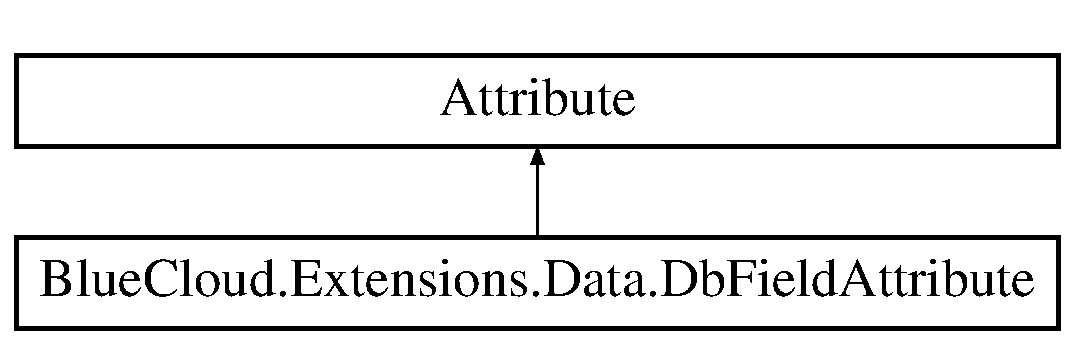
\includegraphics[height=2.000000cm]{class_blue_cloud_1_1_extensions_1_1_data_1_1_db_field_attribute}
\end{center}
\end{figure}
\subsection*{Public Member Functions}
\begin{DoxyCompactItemize}
\item 
\mbox{\hyperlink{class_blue_cloud_1_1_extensions_1_1_data_1_1_db_field_attribute_a215a03bd00877393b57b061cbf6fdc85}{Db\+Field\+Attribute}} (string field\+Name, string parameter\+Name=null)
\begin{DoxyCompactList}\small\item\em Database Field to Property Mapping Attribute \end{DoxyCompactList}\item 
\mbox{\hyperlink{class_blue_cloud_1_1_extensions_1_1_data_1_1_db_field_attribute_ab2236b1aa5c73e738bd5eae507aeb3e5}{Db\+Field\+Attribute}} ()
\begin{DoxyCompactList}\small\item\em Database Field to Property Mapping Attribute. \end{DoxyCompactList}\end{DoxyCompactItemize}
\subsection*{Properties}
\begin{DoxyCompactItemize}
\item 
string \mbox{\hyperlink{class_blue_cloud_1_1_extensions_1_1_data_1_1_db_field_attribute_a146fcf50500222d224a12e27dd4c2285}{Field}}\hspace{0.3cm}{\ttfamily  \mbox{[}get\mbox{]}}
\begin{DoxyCompactList}\small\item\em Database Field \end{DoxyCompactList}\item 
string \mbox{\hyperlink{class_blue_cloud_1_1_extensions_1_1_data_1_1_db_field_attribute_a87545da9d89ae282b3ade4616b960938}{Sql\+Parameter\+Name}}\hspace{0.3cm}{\ttfamily  \mbox{[}get\mbox{]}}
\begin{DoxyCompactList}\small\item\em S\+QL Parameter Name (Optional) in S\+QL Text \end{DoxyCompactList}\end{DoxyCompactItemize}


\subsection{Detailed Description}
Db\+Field Attribute used to annotate properties to be mapped to database fields. 



\subsection{Constructor \& Destructor Documentation}
\mbox{\Hypertarget{class_blue_cloud_1_1_extensions_1_1_data_1_1_db_field_attribute_a215a03bd00877393b57b061cbf6fdc85}\label{class_blue_cloud_1_1_extensions_1_1_data_1_1_db_field_attribute_a215a03bd00877393b57b061cbf6fdc85}} 
\index{Blue\+Cloud\+::\+Extensions\+::\+Data\+::\+Db\+Field\+Attribute@{Blue\+Cloud\+::\+Extensions\+::\+Data\+::\+Db\+Field\+Attribute}!Db\+Field\+Attribute@{Db\+Field\+Attribute}}
\index{Db\+Field\+Attribute@{Db\+Field\+Attribute}!Blue\+Cloud\+::\+Extensions\+::\+Data\+::\+Db\+Field\+Attribute@{Blue\+Cloud\+::\+Extensions\+::\+Data\+::\+Db\+Field\+Attribute}}
\subsubsection{\texorpdfstring{Db\+Field\+Attribute()}{DbFieldAttribute()}\hspace{0.1cm}{\footnotesize\ttfamily [1/2]}}
{\footnotesize\ttfamily Blue\+Cloud.\+Extensions.\+Data.\+Db\+Field\+Attribute.\+Db\+Field\+Attribute (\begin{DoxyParamCaption}\item[{string}]{field\+Name,  }\item[{string}]{parameter\+Name = {\ttfamily null} }\end{DoxyParamCaption})\hspace{0.3cm}{\ttfamily [inline]}}



Database Field to Property Mapping Attribute 

If not specified, the database field will be the property name. 


\begin{DoxyParams}{Parameters}
{\em field\+Name} & Database Field\\
\hline
{\em parameter\+Name} & S\+QL Parameter Name (Optional) in S\+QL Text\\
\hline
\end{DoxyParams}
\mbox{\Hypertarget{class_blue_cloud_1_1_extensions_1_1_data_1_1_db_field_attribute_ab2236b1aa5c73e738bd5eae507aeb3e5}\label{class_blue_cloud_1_1_extensions_1_1_data_1_1_db_field_attribute_ab2236b1aa5c73e738bd5eae507aeb3e5}} 
\index{Blue\+Cloud\+::\+Extensions\+::\+Data\+::\+Db\+Field\+Attribute@{Blue\+Cloud\+::\+Extensions\+::\+Data\+::\+Db\+Field\+Attribute}!Db\+Field\+Attribute@{Db\+Field\+Attribute}}
\index{Db\+Field\+Attribute@{Db\+Field\+Attribute}!Blue\+Cloud\+::\+Extensions\+::\+Data\+::\+Db\+Field\+Attribute@{Blue\+Cloud\+::\+Extensions\+::\+Data\+::\+Db\+Field\+Attribute}}
\subsubsection{\texorpdfstring{Db\+Field\+Attribute()}{DbFieldAttribute()}\hspace{0.1cm}{\footnotesize\ttfamily [2/2]}}
{\footnotesize\ttfamily Blue\+Cloud.\+Extensions.\+Data.\+Db\+Field\+Attribute.\+Db\+Field\+Attribute (\begin{DoxyParamCaption}{ }\end{DoxyParamCaption})\hspace{0.3cm}{\ttfamily [inline]}}



Database Field to Property Mapping Attribute. 

If not specified, the database field will be the property name. 

\subsection{Property Documentation}
\mbox{\Hypertarget{class_blue_cloud_1_1_extensions_1_1_data_1_1_db_field_attribute_a146fcf50500222d224a12e27dd4c2285}\label{class_blue_cloud_1_1_extensions_1_1_data_1_1_db_field_attribute_a146fcf50500222d224a12e27dd4c2285}} 
\index{Blue\+Cloud\+::\+Extensions\+::\+Data\+::\+Db\+Field\+Attribute@{Blue\+Cloud\+::\+Extensions\+::\+Data\+::\+Db\+Field\+Attribute}!Field@{Field}}
\index{Field@{Field}!Blue\+Cloud\+::\+Extensions\+::\+Data\+::\+Db\+Field\+Attribute@{Blue\+Cloud\+::\+Extensions\+::\+Data\+::\+Db\+Field\+Attribute}}
\subsubsection{\texorpdfstring{Field}{Field}}
{\footnotesize\ttfamily string Blue\+Cloud.\+Extensions.\+Data.\+Db\+Field\+Attribute.\+Field\hspace{0.3cm}{\ttfamily [get]}}



Database Field 

\mbox{\Hypertarget{class_blue_cloud_1_1_extensions_1_1_data_1_1_db_field_attribute_a87545da9d89ae282b3ade4616b960938}\label{class_blue_cloud_1_1_extensions_1_1_data_1_1_db_field_attribute_a87545da9d89ae282b3ade4616b960938}} 
\index{Blue\+Cloud\+::\+Extensions\+::\+Data\+::\+Db\+Field\+Attribute@{Blue\+Cloud\+::\+Extensions\+::\+Data\+::\+Db\+Field\+Attribute}!Sql\+Parameter\+Name@{Sql\+Parameter\+Name}}
\index{Sql\+Parameter\+Name@{Sql\+Parameter\+Name}!Blue\+Cloud\+::\+Extensions\+::\+Data\+::\+Db\+Field\+Attribute@{Blue\+Cloud\+::\+Extensions\+::\+Data\+::\+Db\+Field\+Attribute}}
\subsubsection{\texorpdfstring{Sql\+Parameter\+Name}{SqlParameterName}}
{\footnotesize\ttfamily string Blue\+Cloud.\+Extensions.\+Data.\+Db\+Field\+Attribute.\+Sql\+Parameter\+Name\hspace{0.3cm}{\ttfamily [get]}}



S\+QL Parameter Name (Optional) in S\+QL Text 



The documentation for this class was generated from the following file\+:\begin{DoxyCompactItemize}
\item 
Blue\+Cloud.\+Extensions/\+Data/Db\+Field\+Attribute.\+cs\end{DoxyCompactItemize}

\hypertarget{class_blue_cloud_1_1_extensions_1_1_data_1_1_db_mapping}{}\section{Blue\+Cloud.\+Extensions.\+Data.\+Db\+Mapping Class Reference}
\label{class_blue_cloud_1_1_extensions_1_1_data_1_1_db_mapping}\index{Blue\+Cloud.\+Extensions.\+Data.\+Db\+Mapping@{Blue\+Cloud.\+Extensions.\+Data.\+Db\+Mapping}}


Db mapping.  


\subsection*{Properties}
\begin{DoxyCompactItemize}
\item 
string \mbox{\hyperlink{class_blue_cloud_1_1_extensions_1_1_data_1_1_db_mapping_a1fbf6098300d148f91008076c86df606}{Database\+Field}}\hspace{0.3cm}{\ttfamily  \mbox{[}get, set\mbox{]}}
\begin{DoxyCompactList}\small\item\em Mapped Database Field \end{DoxyCompactList}\item 
Property\+Info \mbox{\hyperlink{class_blue_cloud_1_1_extensions_1_1_data_1_1_db_mapping_a33404ee5850071ce4595ff117ed679e6}{Object\+Property}}\hspace{0.3cm}{\ttfamily  \mbox{[}get, set\mbox{]}}
\begin{DoxyCompactList}\small\item\em Reflected Object Property \end{DoxyCompactList}\item 
bool \mbox{\hyperlink{class_blue_cloud_1_1_extensions_1_1_data_1_1_db_mapping_a2346e649c588333fed4639dd9ac72a4c}{Is\+Nullable}}\hspace{0.3cm}{\ttfamily  \mbox{[}get, set\mbox{]}}
\begin{DoxyCompactList}\small\item\em Whether the Reflected Object Property is a Nullable type. \end{DoxyCompactList}\end{DoxyCompactItemize}


\subsection{Detailed Description}
Db mapping. 



\subsection{Property Documentation}
\mbox{\Hypertarget{class_blue_cloud_1_1_extensions_1_1_data_1_1_db_mapping_a1fbf6098300d148f91008076c86df606}\label{class_blue_cloud_1_1_extensions_1_1_data_1_1_db_mapping_a1fbf6098300d148f91008076c86df606}} 
\index{Blue\+Cloud\+::\+Extensions\+::\+Data\+::\+Db\+Mapping@{Blue\+Cloud\+::\+Extensions\+::\+Data\+::\+Db\+Mapping}!Database\+Field@{Database\+Field}}
\index{Database\+Field@{Database\+Field}!Blue\+Cloud\+::\+Extensions\+::\+Data\+::\+Db\+Mapping@{Blue\+Cloud\+::\+Extensions\+::\+Data\+::\+Db\+Mapping}}
\subsubsection{\texorpdfstring{Database\+Field}{DatabaseField}}
{\footnotesize\ttfamily string Blue\+Cloud.\+Extensions.\+Data.\+Db\+Mapping.\+Database\+Field\hspace{0.3cm}{\ttfamily [get]}, {\ttfamily [set]}}



Mapped Database Field 

The database field.\mbox{\Hypertarget{class_blue_cloud_1_1_extensions_1_1_data_1_1_db_mapping_a2346e649c588333fed4639dd9ac72a4c}\label{class_blue_cloud_1_1_extensions_1_1_data_1_1_db_mapping_a2346e649c588333fed4639dd9ac72a4c}} 
\index{Blue\+Cloud\+::\+Extensions\+::\+Data\+::\+Db\+Mapping@{Blue\+Cloud\+::\+Extensions\+::\+Data\+::\+Db\+Mapping}!Is\+Nullable@{Is\+Nullable}}
\index{Is\+Nullable@{Is\+Nullable}!Blue\+Cloud\+::\+Extensions\+::\+Data\+::\+Db\+Mapping@{Blue\+Cloud\+::\+Extensions\+::\+Data\+::\+Db\+Mapping}}
\subsubsection{\texorpdfstring{Is\+Nullable}{IsNullable}}
{\footnotesize\ttfamily bool Blue\+Cloud.\+Extensions.\+Data.\+Db\+Mapping.\+Is\+Nullable\hspace{0.3cm}{\ttfamily [get]}, {\ttfamily [set]}}



Whether the Reflected Object Property is a Nullable type. 

Whether or not the data type is nullable.\mbox{\Hypertarget{class_blue_cloud_1_1_extensions_1_1_data_1_1_db_mapping_a33404ee5850071ce4595ff117ed679e6}\label{class_blue_cloud_1_1_extensions_1_1_data_1_1_db_mapping_a33404ee5850071ce4595ff117ed679e6}} 
\index{Blue\+Cloud\+::\+Extensions\+::\+Data\+::\+Db\+Mapping@{Blue\+Cloud\+::\+Extensions\+::\+Data\+::\+Db\+Mapping}!Object\+Property@{Object\+Property}}
\index{Object\+Property@{Object\+Property}!Blue\+Cloud\+::\+Extensions\+::\+Data\+::\+Db\+Mapping@{Blue\+Cloud\+::\+Extensions\+::\+Data\+::\+Db\+Mapping}}
\subsubsection{\texorpdfstring{Object\+Property}{ObjectProperty}}
{\footnotesize\ttfamily Property\+Info Blue\+Cloud.\+Extensions.\+Data.\+Db\+Mapping.\+Object\+Property\hspace{0.3cm}{\ttfamily [get]}, {\ttfamily [set]}}



Reflected Object Property 

Property\+Info of a property

The documentation for this class was generated from the following file\+:\begin{DoxyCompactItemize}
\item 
Blue\+Cloud.\+Extensions/\+Data/Db\+Mapping.\+cs\end{DoxyCompactItemize}

\hypertarget{class_blue_cloud_1_1_extensions_1_1_cache_1_1_default_cache}{}\section{Blue\+Cloud.\+Extensions.\+Cache.\+Default\+Cache$<$ T $>$ Class Template Reference}
\label{class_blue_cloud_1_1_extensions_1_1_cache_1_1_default_cache}\index{Blue\+Cloud.\+Extensions.\+Cache.\+Default\+Cache$<$ T $>$@{Blue\+Cloud.\+Extensions.\+Cache.\+Default\+Cache$<$ T $>$}}


Default cache utilizing System.\+Runtime.\+Caching.\+Memory\+Cache  


Inheritance diagram for Blue\+Cloud.\+Extensions.\+Cache.\+Default\+Cache$<$ T $>$\+:\begin{figure}[H]
\begin{center}
\leavevmode
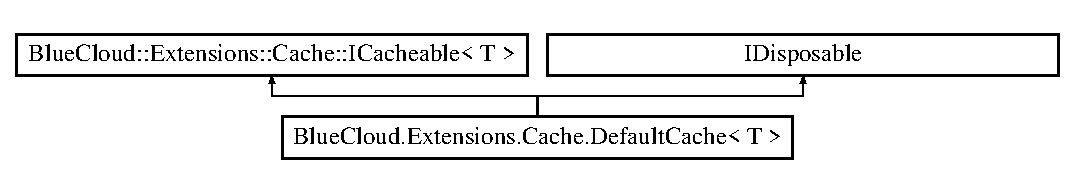
\includegraphics[height=1.898305cm]{class_blue_cloud_1_1_extensions_1_1_cache_1_1_default_cache}
\end{center}
\end{figure}
\subsection*{Public Member Functions}
\begin{DoxyCompactItemize}
\item 
\mbox{\hyperlink{class_blue_cloud_1_1_extensions_1_1_cache_1_1_default_cache_a14fec20f91a78d445887fab2f59cfc7c}{Default\+Cache}} (Time\+Span sliding\+Expiration)
\begin{DoxyCompactList}\small\item\em Initializes a new instance of the T\+:\+Blue\+Cloud.\+Extensions.\+Cache.\+Default\+Cache\`{}1 class. \end{DoxyCompactList}\item 
void \mbox{\hyperlink{class_blue_cloud_1_1_extensions_1_1_cache_1_1_default_cache_a4ce78dfa582354a24038b9e94bdd750f}{Dispose}} ()
\begin{DoxyCompactList}\small\item\em Releases all resource used by the T\+:\+Blue\+Cloud.\+Extensions.\+Cache.\+Default\+Cache\`{}1 object. \end{DoxyCompactList}\item 
T \mbox{\hyperlink{class_blue_cloud_1_1_extensions_1_1_cache_1_1_default_cache_a93bb4ec6f9ec285c1d13a9f44ed3e48f}{Get}} (string key)
\begin{DoxyCompactList}\small\item\em Get cached object with specified key. \end{DoxyCompactList}\item 
void \mbox{\hyperlink{class_blue_cloud_1_1_extensions_1_1_cache_1_1_default_cache_a516484e43036468f7258451139938798}{Set}} (string key, T value)
\begin{DoxyCompactList}\small\item\em Caches an object with specified key. \end{DoxyCompactList}\end{DoxyCompactItemize}
\subsection*{Properties}
\begin{DoxyCompactItemize}
\item 
\mbox{\Hypertarget{class_blue_cloud_1_1_extensions_1_1_cache_1_1_default_cache_ab3a9a9c08e2dcb3f621b0a6e26a7e56d}\label{class_blue_cloud_1_1_extensions_1_1_cache_1_1_default_cache_ab3a9a9c08e2dcb3f621b0a6e26a7e56d}} 
Time\+Span {\bfseries Sliding\+Expiration}\hspace{0.3cm}{\ttfamily  \mbox{[}get, set\mbox{]}}
\end{DoxyCompactItemize}


\subsection{Detailed Description}
Default cache utilizing System.\+Runtime.\+Caching.\+Memory\+Cache 



\subsection{Constructor \& Destructor Documentation}
\mbox{\Hypertarget{class_blue_cloud_1_1_extensions_1_1_cache_1_1_default_cache_a14fec20f91a78d445887fab2f59cfc7c}\label{class_blue_cloud_1_1_extensions_1_1_cache_1_1_default_cache_a14fec20f91a78d445887fab2f59cfc7c}} 
\index{Blue\+Cloud\+::\+Extensions\+::\+Cache\+::\+Default\+Cache@{Blue\+Cloud\+::\+Extensions\+::\+Cache\+::\+Default\+Cache}!Default\+Cache@{Default\+Cache}}
\index{Default\+Cache@{Default\+Cache}!Blue\+Cloud\+::\+Extensions\+::\+Cache\+::\+Default\+Cache@{Blue\+Cloud\+::\+Extensions\+::\+Cache\+::\+Default\+Cache}}
\subsubsection{\texorpdfstring{Default\+Cache()}{DefaultCache()}}
{\footnotesize\ttfamily \mbox{\hyperlink{class_blue_cloud_1_1_extensions_1_1_cache_1_1_default_cache}{Blue\+Cloud.\+Extensions.\+Cache.\+Default\+Cache}}$<$ T $>$.\mbox{\hyperlink{class_blue_cloud_1_1_extensions_1_1_cache_1_1_default_cache}{Default\+Cache}} (\begin{DoxyParamCaption}\item[{Time\+Span}]{sliding\+Expiration }\end{DoxyParamCaption})\hspace{0.3cm}{\ttfamily [inline]}}



Initializes a new instance of the T\+:\+Blue\+Cloud.\+Extensions.\+Cache.\+Default\+Cache\`{}1 class. 


\begin{DoxyParams}{Parameters}
{\em sliding\+Expiration} & Sliding Expiration\\
\hline
\end{DoxyParams}


\subsection{Member Function Documentation}
\mbox{\Hypertarget{class_blue_cloud_1_1_extensions_1_1_cache_1_1_default_cache_a4ce78dfa582354a24038b9e94bdd750f}\label{class_blue_cloud_1_1_extensions_1_1_cache_1_1_default_cache_a4ce78dfa582354a24038b9e94bdd750f}} 
\index{Blue\+Cloud\+::\+Extensions\+::\+Cache\+::\+Default\+Cache@{Blue\+Cloud\+::\+Extensions\+::\+Cache\+::\+Default\+Cache}!Dispose@{Dispose}}
\index{Dispose@{Dispose}!Blue\+Cloud\+::\+Extensions\+::\+Cache\+::\+Default\+Cache@{Blue\+Cloud\+::\+Extensions\+::\+Cache\+::\+Default\+Cache}}
\subsubsection{\texorpdfstring{Dispose()}{Dispose()}}
{\footnotesize\ttfamily void \mbox{\hyperlink{class_blue_cloud_1_1_extensions_1_1_cache_1_1_default_cache}{Blue\+Cloud.\+Extensions.\+Cache.\+Default\+Cache}}$<$ T $>$.Dispose (\begin{DoxyParamCaption}{ }\end{DoxyParamCaption})\hspace{0.3cm}{\ttfamily [inline]}}



Releases all resource used by the T\+:\+Blue\+Cloud.\+Extensions.\+Cache.\+Default\+Cache\`{}1 object. 

Call \mbox{\hyperlink{class_blue_cloud_1_1_extensions_1_1_cache_1_1_default_cache_a4ce78dfa582354a24038b9e94bdd750f}{Dispose}} when you are finished using the T\+:\+Blue\+Cloud.\+Extensions.\+Cache.\+Default\+Cache\`{}1. The \mbox{\hyperlink{class_blue_cloud_1_1_extensions_1_1_cache_1_1_default_cache_a4ce78dfa582354a24038b9e94bdd750f}{Dispose}} method leaves the T\+:\+Blue\+Cloud.\+Extensions.\+Cache.\+Default\+Cache\`{}1 in an unusable state. After calling \mbox{\hyperlink{class_blue_cloud_1_1_extensions_1_1_cache_1_1_default_cache_a4ce78dfa582354a24038b9e94bdd750f}{Dispose}}, you must release all references to the T\+:\+Blue\+Cloud.\+Extensions.\+Cache.\+Default\+Cache\`{}1 so the garbage collector can reclaim the memory that the T\+:\+Blue\+Cloud.\+Extensions.\+Cache.\+Default\+Cache\`{}1 was occupying.\mbox{\Hypertarget{class_blue_cloud_1_1_extensions_1_1_cache_1_1_default_cache_a93bb4ec6f9ec285c1d13a9f44ed3e48f}\label{class_blue_cloud_1_1_extensions_1_1_cache_1_1_default_cache_a93bb4ec6f9ec285c1d13a9f44ed3e48f}} 
\index{Blue\+Cloud\+::\+Extensions\+::\+Cache\+::\+Default\+Cache@{Blue\+Cloud\+::\+Extensions\+::\+Cache\+::\+Default\+Cache}!Get@{Get}}
\index{Get@{Get}!Blue\+Cloud\+::\+Extensions\+::\+Cache\+::\+Default\+Cache@{Blue\+Cloud\+::\+Extensions\+::\+Cache\+::\+Default\+Cache}}
\subsubsection{\texorpdfstring{Get()}{Get()}}
{\footnotesize\ttfamily T \mbox{\hyperlink{class_blue_cloud_1_1_extensions_1_1_cache_1_1_default_cache}{Blue\+Cloud.\+Extensions.\+Cache.\+Default\+Cache}}$<$ T $>$.Get (\begin{DoxyParamCaption}\item[{string}]{key }\end{DoxyParamCaption})\hspace{0.3cm}{\ttfamily [inline]}}



Get cached object with specified key. 

\begin{DoxyReturn}{Returns}
Cached object
\end{DoxyReturn}

\begin{DoxyParams}{Parameters}
{\em key} & Key\\
\hline
\end{DoxyParams}


Implements \mbox{\hyperlink{interface_blue_cloud_1_1_extensions_1_1_cache_1_1_i_cacheable_aadcdce6338f6c4aaafc6c3068c4b6dc1}{Blue\+Cloud.\+Extensions.\+Cache.\+I\+Cacheable$<$ T $>$}}.

\mbox{\Hypertarget{class_blue_cloud_1_1_extensions_1_1_cache_1_1_default_cache_a516484e43036468f7258451139938798}\label{class_blue_cloud_1_1_extensions_1_1_cache_1_1_default_cache_a516484e43036468f7258451139938798}} 
\index{Blue\+Cloud\+::\+Extensions\+::\+Cache\+::\+Default\+Cache@{Blue\+Cloud\+::\+Extensions\+::\+Cache\+::\+Default\+Cache}!Set@{Set}}
\index{Set@{Set}!Blue\+Cloud\+::\+Extensions\+::\+Cache\+::\+Default\+Cache@{Blue\+Cloud\+::\+Extensions\+::\+Cache\+::\+Default\+Cache}}
\subsubsection{\texorpdfstring{Set()}{Set()}}
{\footnotesize\ttfamily void \mbox{\hyperlink{class_blue_cloud_1_1_extensions_1_1_cache_1_1_default_cache}{Blue\+Cloud.\+Extensions.\+Cache.\+Default\+Cache}}$<$ T $>$.Set (\begin{DoxyParamCaption}\item[{string}]{key,  }\item[{T}]{value }\end{DoxyParamCaption})\hspace{0.3cm}{\ttfamily [inline]}}



Caches an object with specified key. 


\begin{DoxyParams}{Parameters}
{\em key} & Key\\
\hline
{\em value} & Value\\
\hline
\end{DoxyParams}


Implements \mbox{\hyperlink{interface_blue_cloud_1_1_extensions_1_1_cache_1_1_i_cacheable_a668a7dff25dcd6a612830c4d15fe73cb}{Blue\+Cloud.\+Extensions.\+Cache.\+I\+Cacheable$<$ T $>$}}.



The documentation for this class was generated from the following file\+:\begin{DoxyCompactItemize}
\item 
Blue\+Cloud.\+Extensions/\+Cache/Default\+Cache.\+cs\end{DoxyCompactItemize}

\hypertarget{interface_blue_cloud_1_1_extensions_1_1_cache_1_1_i_cacheable}{}\section{Blue\+Cloud.\+Extensions.\+Cache.\+I\+Cacheable$<$ T $>$ Interface Template Reference}
\label{interface_blue_cloud_1_1_extensions_1_1_cache_1_1_i_cacheable}\index{Blue\+Cloud.\+Extensions.\+Cache.\+I\+Cacheable$<$ T $>$@{Blue\+Cloud.\+Extensions.\+Cache.\+I\+Cacheable$<$ T $>$}}


\mbox{\hyperlink{interface_blue_cloud_1_1_extensions_1_1_cache_1_1_i_cacheable}{I\+Cacheable}} Interface used for caching database field to object property mappings. Customize caching with your own implementation.  


Inheritance diagram for Blue\+Cloud.\+Extensions.\+Cache.\+I\+Cacheable$<$ T $>$\+:\begin{figure}[H]
\begin{center}
\leavevmode
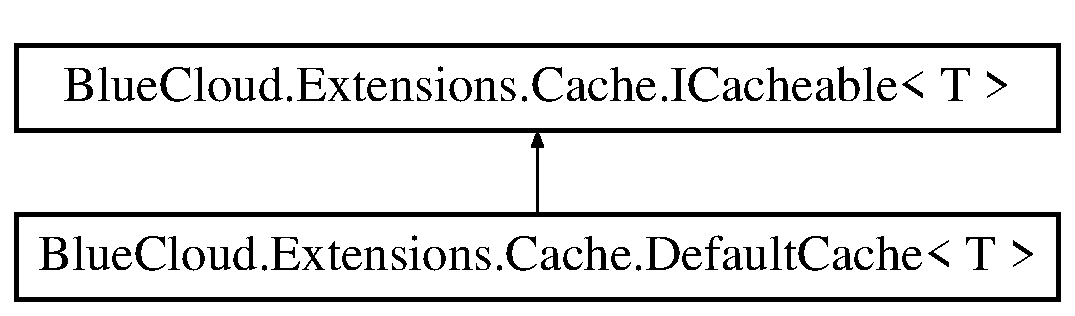
\includegraphics[height=2.000000cm]{interface_blue_cloud_1_1_extensions_1_1_cache_1_1_i_cacheable}
\end{center}
\end{figure}
\subsection*{Public Member Functions}
\begin{DoxyCompactItemize}
\item 
T \mbox{\hyperlink{interface_blue_cloud_1_1_extensions_1_1_cache_1_1_i_cacheable_aadcdce6338f6c4aaafc6c3068c4b6dc1}{Get}} (string key)
\begin{DoxyCompactList}\small\item\em Get cached object with specified key. \end{DoxyCompactList}\item 
void \mbox{\hyperlink{interface_blue_cloud_1_1_extensions_1_1_cache_1_1_i_cacheable_a668a7dff25dcd6a612830c4d15fe73cb}{Set}} (string key, T value)
\begin{DoxyCompactList}\small\item\em Caches an object with specified key. \end{DoxyCompactList}\end{DoxyCompactItemize}


\subsection{Detailed Description}
\mbox{\hyperlink{interface_blue_cloud_1_1_extensions_1_1_cache_1_1_i_cacheable}{I\+Cacheable}} Interface used for caching database field to object property mappings. Customize caching with your own implementation. 



\subsection{Member Function Documentation}
\mbox{\Hypertarget{interface_blue_cloud_1_1_extensions_1_1_cache_1_1_i_cacheable_aadcdce6338f6c4aaafc6c3068c4b6dc1}\label{interface_blue_cloud_1_1_extensions_1_1_cache_1_1_i_cacheable_aadcdce6338f6c4aaafc6c3068c4b6dc1}} 
\index{Blue\+Cloud\+::\+Extensions\+::\+Cache\+::\+I\+Cacheable@{Blue\+Cloud\+::\+Extensions\+::\+Cache\+::\+I\+Cacheable}!Get@{Get}}
\index{Get@{Get}!Blue\+Cloud\+::\+Extensions\+::\+Cache\+::\+I\+Cacheable@{Blue\+Cloud\+::\+Extensions\+::\+Cache\+::\+I\+Cacheable}}
\subsubsection{\texorpdfstring{Get()}{Get()}}
{\footnotesize\ttfamily T \mbox{\hyperlink{interface_blue_cloud_1_1_extensions_1_1_cache_1_1_i_cacheable}{Blue\+Cloud.\+Extensions.\+Cache.\+I\+Cacheable}}$<$ T $>$.Get (\begin{DoxyParamCaption}\item[{string}]{key }\end{DoxyParamCaption})}



Get cached object with specified key. 

\begin{DoxyReturn}{Returns}
Cached object
\end{DoxyReturn}

\begin{DoxyParams}{Parameters}
{\em key} & Key\\
\hline
\end{DoxyParams}


Implemented in \mbox{\hyperlink{class_blue_cloud_1_1_extensions_1_1_cache_1_1_default_cache_a93bb4ec6f9ec285c1d13a9f44ed3e48f}{Blue\+Cloud.\+Extensions.\+Cache.\+Default\+Cache$<$ T $>$}}.

\mbox{\Hypertarget{interface_blue_cloud_1_1_extensions_1_1_cache_1_1_i_cacheable_a668a7dff25dcd6a612830c4d15fe73cb}\label{interface_blue_cloud_1_1_extensions_1_1_cache_1_1_i_cacheable_a668a7dff25dcd6a612830c4d15fe73cb}} 
\index{Blue\+Cloud\+::\+Extensions\+::\+Cache\+::\+I\+Cacheable@{Blue\+Cloud\+::\+Extensions\+::\+Cache\+::\+I\+Cacheable}!Set@{Set}}
\index{Set@{Set}!Blue\+Cloud\+::\+Extensions\+::\+Cache\+::\+I\+Cacheable@{Blue\+Cloud\+::\+Extensions\+::\+Cache\+::\+I\+Cacheable}}
\subsubsection{\texorpdfstring{Set()}{Set()}}
{\footnotesize\ttfamily void \mbox{\hyperlink{interface_blue_cloud_1_1_extensions_1_1_cache_1_1_i_cacheable}{Blue\+Cloud.\+Extensions.\+Cache.\+I\+Cacheable}}$<$ T $>$.Set (\begin{DoxyParamCaption}\item[{string}]{key,  }\item[{T}]{value }\end{DoxyParamCaption})}



Caches an object with specified key. 


\begin{DoxyParams}{Parameters}
{\em key} & Key\\
\hline
{\em value} & Value\\
\hline
\end{DoxyParams}


Implemented in \mbox{\hyperlink{class_blue_cloud_1_1_extensions_1_1_cache_1_1_default_cache_a516484e43036468f7258451139938798}{Blue\+Cloud.\+Extensions.\+Cache.\+Default\+Cache$<$ T $>$}}.



The documentation for this interface was generated from the following file\+:\begin{DoxyCompactItemize}
\item 
Blue\+Cloud.\+Extensions/\+Cache/I\+Cacheable.\+cs\end{DoxyCompactItemize}

\hypertarget{class_blue_cloud_1_1_extensions_1_1_data_1_1_i_data_reader_extensions}{}\section{Blue\+Cloud.\+Extensions.\+Data.\+I\+Data\+Reader\+Extensions Class Reference}
\label{class_blue_cloud_1_1_extensions_1_1_data_1_1_i_data_reader_extensions}\index{Blue\+Cloud.\+Extensions.\+Data.\+I\+Data\+Reader\+Extensions@{Blue\+Cloud.\+Extensions.\+Data.\+I\+Data\+Reader\+Extensions}}


Extension Methods for System.\+Data.\+I\+Data\+Reader  


\subsection*{Static Public Member Functions}
\begin{DoxyCompactItemize}
\item 
static T \mbox{\hyperlink{class_blue_cloud_1_1_extensions_1_1_data_1_1_i_data_reader_extensions_a9f0ec28408443dd8a53d3eebb81e4dda}{Get\+Value$<$ T $>$}} (this I\+Data\+Reader data\+Reader, string field\+Name)
\begin{DoxyCompactList}\small\item\em Returns a value from the database with a given type. \end{DoxyCompactList}\item 
static I\+Enumerable$<$ T $>$ \mbox{\hyperlink{class_blue_cloud_1_1_extensions_1_1_data_1_1_i_data_reader_extensions_a96d6babf950003a62ab3dab97d868c53}{Map\+To\+Objects$<$ T $>$}} (this I\+Data\+Reader data\+Reader)
\begin{DoxyCompactList}\small\item\em Maps a data reader result to model classes \end{DoxyCompactList}\item 
static I\+Enumerable$<$ Tuple$<$ T, U $>$ $>$ \mbox{\hyperlink{class_blue_cloud_1_1_extensions_1_1_data_1_1_i_data_reader_extensions_af125bc42a7dc02955ce4322f138c8648}{Map\+To\+Objects$<$ T, U $>$}} (this I\+Data\+Reader data\+Reader)
\begin{DoxyCompactList}\small\item\em Maps a data reader result to model classes \end{DoxyCompactList}\item 
static I\+Enumerable$<$ T $>$ \mbox{\hyperlink{class_blue_cloud_1_1_extensions_1_1_data_1_1_i_data_reader_extensions_a4cb93e1c624aa13c212084880c57c243}{Map\+To\+Objects$<$ T $>$}} (this I\+Data\+Reader data\+Reader, int take)
\begin{DoxyCompactList}\small\item\em Maps a data reader result to model classes \end{DoxyCompactList}\item 
static I\+Enumerable$<$ Tuple$<$ T, U $>$ $>$ \mbox{\hyperlink{class_blue_cloud_1_1_extensions_1_1_data_1_1_i_data_reader_extensions_ac1ab442430a138f00d6845d5d7b30241}{Map\+To\+Objects$<$ T, U $>$}} (this I\+Data\+Reader data\+Reader, int take)
\begin{DoxyCompactList}\small\item\em Maps to objects. \end{DoxyCompactList}\item 
static Dictionary$<$ string, int $>$ \mbox{\hyperlink{class_blue_cloud_1_1_extensions_1_1_data_1_1_i_data_reader_extensions_a6f7b4f6e3b78a8a6eea6bcd8927c5531}{Get\+Column\+Ordinals}} (this I\+Data\+Record record)
\begin{DoxyCompactList}\small\item\em Returns a dictionary mapping of a database field name to column ordinal. \end{DoxyCompactList}\end{DoxyCompactItemize}
\subsection*{Static Public Attributes}
\begin{DoxyCompactItemize}
\item 
static \mbox{\hyperlink{interface_blue_cloud_1_1_extensions_1_1_cache_1_1_i_cacheable}{I\+Cacheable}}$<$ List$<$ \mbox{\hyperlink{class_blue_cloud_1_1_extensions_1_1_data_1_1_db_mapping}{Db\+Mapping}} $>$ $>$ \mbox{\hyperlink{class_blue_cloud_1_1_extensions_1_1_data_1_1_i_data_reader_extensions_aec5e45db6160d2502c2eceead22b1a83}{cache}} = new \mbox{\hyperlink{class_blue_cloud_1_1_extensions_1_1_cache_1_1_default_cache}{Default\+Cache}}$<$List$<$\mbox{\hyperlink{class_blue_cloud_1_1_extensions_1_1_data_1_1_db_mapping}{Db\+Mapping}}$>$$>$(new Time\+Span(2, 0, 0))
\begin{DoxyCompactList}\small\item\em I\+Cacheable interface used to cache reflected property information. By default, items are cached in a sliding 2 hour window. \end{DoxyCompactList}\end{DoxyCompactItemize}


\subsection{Detailed Description}
Extension Methods for System.\+Data.\+I\+Data\+Reader 



\subsection{Member Function Documentation}
\mbox{\Hypertarget{class_blue_cloud_1_1_extensions_1_1_data_1_1_i_data_reader_extensions_a6f7b4f6e3b78a8a6eea6bcd8927c5531}\label{class_blue_cloud_1_1_extensions_1_1_data_1_1_i_data_reader_extensions_a6f7b4f6e3b78a8a6eea6bcd8927c5531}} 
\index{Blue\+Cloud\+::\+Extensions\+::\+Data\+::\+I\+Data\+Reader\+Extensions@{Blue\+Cloud\+::\+Extensions\+::\+Data\+::\+I\+Data\+Reader\+Extensions}!Get\+Column\+Ordinals@{Get\+Column\+Ordinals}}
\index{Get\+Column\+Ordinals@{Get\+Column\+Ordinals}!Blue\+Cloud\+::\+Extensions\+::\+Data\+::\+I\+Data\+Reader\+Extensions@{Blue\+Cloud\+::\+Extensions\+::\+Data\+::\+I\+Data\+Reader\+Extensions}}
\subsubsection{\texorpdfstring{Get\+Column\+Ordinals()}{GetColumnOrdinals()}}
{\footnotesize\ttfamily static Dictionary$<$string, int$>$ Blue\+Cloud.\+Extensions.\+Data.\+I\+Data\+Reader\+Extensions.\+Get\+Column\+Ordinals (\begin{DoxyParamCaption}\item[{this I\+Data\+Record}]{record }\end{DoxyParamCaption})\hspace{0.3cm}{\ttfamily [inline]}, {\ttfamily [static]}}



Returns a dictionary mapping of a database field name to column ordinal. 

\begin{DoxyReturn}{Returns}
Mapping of field name to column ordinal
\end{DoxyReturn}

\begin{DoxyParams}{Parameters}
{\em record} & \mbox{\hyperlink{namespace_blue_cloud_1_1_extensions_1_1_data}{Data}} Record\\
\hline
\end{DoxyParams}
\mbox{\Hypertarget{class_blue_cloud_1_1_extensions_1_1_data_1_1_i_data_reader_extensions_a9f0ec28408443dd8a53d3eebb81e4dda}\label{class_blue_cloud_1_1_extensions_1_1_data_1_1_i_data_reader_extensions_a9f0ec28408443dd8a53d3eebb81e4dda}} 
\index{Blue\+Cloud\+::\+Extensions\+::\+Data\+::\+I\+Data\+Reader\+Extensions@{Blue\+Cloud\+::\+Extensions\+::\+Data\+::\+I\+Data\+Reader\+Extensions}!Get\+Value$<$ T $>$@{Get\+Value$<$ T $>$}}
\index{Get\+Value$<$ T $>$@{Get\+Value$<$ T $>$}!Blue\+Cloud\+::\+Extensions\+::\+Data\+::\+I\+Data\+Reader\+Extensions@{Blue\+Cloud\+::\+Extensions\+::\+Data\+::\+I\+Data\+Reader\+Extensions}}
\subsubsection{\texorpdfstring{Get\+Value$<$ T $>$()}{GetValue< T >()}}
{\footnotesize\ttfamily static T Blue\+Cloud.\+Extensions.\+Data.\+I\+Data\+Reader\+Extensions.\+Get\+Value$<$ T $>$ (\begin{DoxyParamCaption}\item[{this I\+Data\+Reader}]{data\+Reader,  }\item[{string}]{field\+Name }\end{DoxyParamCaption})\hspace{0.3cm}{\ttfamily [inline]}, {\ttfamily [static]}}



Returns a value from the database with a given type. 


\begin{DoxyTemplParams}{Template Parameters}
{\em T} & \mbox{\hyperlink{namespace_blue_cloud_1_1_extensions_1_1_data}{Data}} Type\\
\hline
\end{DoxyTemplParams}

\begin{DoxyParams}{Parameters}
{\em field\+Name} & Database Field Name\\
\hline
\end{DoxyParams}
\begin{DoxyReturn}{Returns}
Value from database
\end{DoxyReturn}
\mbox{\Hypertarget{class_blue_cloud_1_1_extensions_1_1_data_1_1_i_data_reader_extensions_a96d6babf950003a62ab3dab97d868c53}\label{class_blue_cloud_1_1_extensions_1_1_data_1_1_i_data_reader_extensions_a96d6babf950003a62ab3dab97d868c53}} 
\index{Blue\+Cloud\+::\+Extensions\+::\+Data\+::\+I\+Data\+Reader\+Extensions@{Blue\+Cloud\+::\+Extensions\+::\+Data\+::\+I\+Data\+Reader\+Extensions}!Map\+To\+Objects$<$ T $>$@{Map\+To\+Objects$<$ T $>$}}
\index{Map\+To\+Objects$<$ T $>$@{Map\+To\+Objects$<$ T $>$}!Blue\+Cloud\+::\+Extensions\+::\+Data\+::\+I\+Data\+Reader\+Extensions@{Blue\+Cloud\+::\+Extensions\+::\+Data\+::\+I\+Data\+Reader\+Extensions}}
\subsubsection{\texorpdfstring{Map\+To\+Objects$<$ T $>$()}{MapToObjects< T >()}\hspace{0.1cm}{\footnotesize\ttfamily [1/2]}}
{\footnotesize\ttfamily static I\+Enumerable$<$T$>$ Blue\+Cloud.\+Extensions.\+Data.\+I\+Data\+Reader\+Extensions.\+Map\+To\+Objects$<$ T $>$ (\begin{DoxyParamCaption}\item[{this I\+Data\+Reader}]{data\+Reader }\end{DoxyParamCaption})\hspace{0.3cm}{\ttfamily [inline]}, {\ttfamily [static]}}



Maps a data reader result to model classes 

\begin{DoxyReturn}{Returns}
Mapped Model Objects
\end{DoxyReturn}

\begin{DoxyParams}{Parameters}
{\em data\+Reader} & \mbox{\hyperlink{namespace_blue_cloud_1_1_extensions_1_1_data}{Data}} reader\\
\hline
\end{DoxyParams}

\begin{DoxyTemplParams}{Template Parameters}
{\em T} & \mbox{\hyperlink{namespace_blue_cloud_1_1_extensions_1_1_data}{Data}} Type\\
\hline
\end{DoxyTemplParams}
\begin{Desc}
\item[Type Constraints]\begin{description}
\item[{\em T} : {\em class}]\end{description}
\end{Desc}
\mbox{\Hypertarget{class_blue_cloud_1_1_extensions_1_1_data_1_1_i_data_reader_extensions_a4cb93e1c624aa13c212084880c57c243}\label{class_blue_cloud_1_1_extensions_1_1_data_1_1_i_data_reader_extensions_a4cb93e1c624aa13c212084880c57c243}} 
\index{Blue\+Cloud\+::\+Extensions\+::\+Data\+::\+I\+Data\+Reader\+Extensions@{Blue\+Cloud\+::\+Extensions\+::\+Data\+::\+I\+Data\+Reader\+Extensions}!Map\+To\+Objects$<$ T $>$@{Map\+To\+Objects$<$ T $>$}}
\index{Map\+To\+Objects$<$ T $>$@{Map\+To\+Objects$<$ T $>$}!Blue\+Cloud\+::\+Extensions\+::\+Data\+::\+I\+Data\+Reader\+Extensions@{Blue\+Cloud\+::\+Extensions\+::\+Data\+::\+I\+Data\+Reader\+Extensions}}
\subsubsection{\texorpdfstring{Map\+To\+Objects$<$ T $>$()}{MapToObjects< T >()}\hspace{0.1cm}{\footnotesize\ttfamily [2/2]}}
{\footnotesize\ttfamily static I\+Enumerable$<$T$>$ Blue\+Cloud.\+Extensions.\+Data.\+I\+Data\+Reader\+Extensions.\+Map\+To\+Objects$<$ T $>$ (\begin{DoxyParamCaption}\item[{this I\+Data\+Reader}]{data\+Reader,  }\item[{int}]{take }\end{DoxyParamCaption})\hspace{0.3cm}{\ttfamily [inline]}, {\ttfamily [static]}}



Maps a data reader result to model classes 

Amount of records to map. A negative 1 (-\/1) will map all records. 

\begin{DoxyReturn}{Returns}
Mapped Model Objects
\end{DoxyReturn}

\begin{DoxyParams}{Parameters}
{\em data\+Reader} & \mbox{\hyperlink{namespace_blue_cloud_1_1_extensions_1_1_data}{Data}} reader\\
\hline
{\em take} & Amount of records to map. A negative 1 (-\/1) will map all records.\\
\hline
\end{DoxyParams}

\begin{DoxyTemplParams}{Template Parameters}
{\em T} & \mbox{\hyperlink{namespace_blue_cloud_1_1_extensions_1_1_data}{Data}} Type\\
\hline
\end{DoxyTemplParams}
\begin{Desc}
\item[Type Constraints]\begin{description}
\item[{\em T} : {\em class}]\end{description}
\end{Desc}
\mbox{\Hypertarget{class_blue_cloud_1_1_extensions_1_1_data_1_1_i_data_reader_extensions_af125bc42a7dc02955ce4322f138c8648}\label{class_blue_cloud_1_1_extensions_1_1_data_1_1_i_data_reader_extensions_af125bc42a7dc02955ce4322f138c8648}} 
\index{Blue\+Cloud\+::\+Extensions\+::\+Data\+::\+I\+Data\+Reader\+Extensions@{Blue\+Cloud\+::\+Extensions\+::\+Data\+::\+I\+Data\+Reader\+Extensions}!Map\+To\+Objects$<$ T, U $>$@{Map\+To\+Objects$<$ T, U $>$}}
\index{Map\+To\+Objects$<$ T, U $>$@{Map\+To\+Objects$<$ T, U $>$}!Blue\+Cloud\+::\+Extensions\+::\+Data\+::\+I\+Data\+Reader\+Extensions@{Blue\+Cloud\+::\+Extensions\+::\+Data\+::\+I\+Data\+Reader\+Extensions}}
\subsubsection{\texorpdfstring{Map\+To\+Objects$<$ T, U $>$()}{MapToObjects< T, U >()}\hspace{0.1cm}{\footnotesize\ttfamily [1/2]}}
{\footnotesize\ttfamily static I\+Enumerable$<$Tuple$<$T, U$>$ $>$ Blue\+Cloud.\+Extensions.\+Data.\+I\+Data\+Reader\+Extensions.\+Map\+To\+Objects$<$ T, U $>$ (\begin{DoxyParamCaption}\item[{this I\+Data\+Reader}]{data\+Reader }\end{DoxyParamCaption})\hspace{0.3cm}{\ttfamily [inline]}, {\ttfamily [static]}}



Maps a data reader result to model classes 

\begin{DoxyReturn}{Returns}
Tuple of Mapped Model Objects
\end{DoxyReturn}

\begin{DoxyParams}{Parameters}
{\em data\+Reader} & \mbox{\hyperlink{namespace_blue_cloud_1_1_extensions_1_1_data}{Data}} reader\\
\hline
\end{DoxyParams}

\begin{DoxyTemplParams}{Template Parameters}
{\em T} & First \mbox{\hyperlink{namespace_blue_cloud_1_1_extensions_1_1_data}{Data}} Type\\
\hline
{\em U} & Second \mbox{\hyperlink{namespace_blue_cloud_1_1_extensions_1_1_data}{Data}} Type\\
\hline
\end{DoxyTemplParams}
\begin{Desc}
\item[Type Constraints]\begin{description}
\item[{\em T} : {\em class}]\item[{\em U} : {\em class}]\end{description}
\end{Desc}
\mbox{\Hypertarget{class_blue_cloud_1_1_extensions_1_1_data_1_1_i_data_reader_extensions_ac1ab442430a138f00d6845d5d7b30241}\label{class_blue_cloud_1_1_extensions_1_1_data_1_1_i_data_reader_extensions_ac1ab442430a138f00d6845d5d7b30241}} 
\index{Blue\+Cloud\+::\+Extensions\+::\+Data\+::\+I\+Data\+Reader\+Extensions@{Blue\+Cloud\+::\+Extensions\+::\+Data\+::\+I\+Data\+Reader\+Extensions}!Map\+To\+Objects$<$ T, U $>$@{Map\+To\+Objects$<$ T, U $>$}}
\index{Map\+To\+Objects$<$ T, U $>$@{Map\+To\+Objects$<$ T, U $>$}!Blue\+Cloud\+::\+Extensions\+::\+Data\+::\+I\+Data\+Reader\+Extensions@{Blue\+Cloud\+::\+Extensions\+::\+Data\+::\+I\+Data\+Reader\+Extensions}}
\subsubsection{\texorpdfstring{Map\+To\+Objects$<$ T, U $>$()}{MapToObjects< T, U >()}\hspace{0.1cm}{\footnotesize\ttfamily [2/2]}}
{\footnotesize\ttfamily static I\+Enumerable$<$Tuple$<$T, U$>$ $>$ Blue\+Cloud.\+Extensions.\+Data.\+I\+Data\+Reader\+Extensions.\+Map\+To\+Objects$<$ T, U $>$ (\begin{DoxyParamCaption}\item[{this I\+Data\+Reader}]{data\+Reader,  }\item[{int}]{take }\end{DoxyParamCaption})\hspace{0.3cm}{\ttfamily [inline]}, {\ttfamily [static]}}



Maps to objects. 

\begin{DoxyReturn}{Returns}
The to objects.
\end{DoxyReturn}

\begin{DoxyParams}{Parameters}
{\em data\+Reader} & \mbox{\hyperlink{namespace_blue_cloud_1_1_extensions_1_1_data}{Data}} reader.\\
\hline
{\em take} & Take.\\
\hline
\end{DoxyParams}

\begin{DoxyTemplParams}{Template Parameters}
{\em T} & The 1st type parameter.\\
\hline
{\em U} & The 2nd type parameter.\\
\hline
\end{DoxyTemplParams}
\begin{Desc}
\item[Type Constraints]\begin{description}
\item[{\em T} : {\em class}]\item[{\em U} : {\em class}]\end{description}
\end{Desc}


\subsection{Member Data Documentation}
\mbox{\Hypertarget{class_blue_cloud_1_1_extensions_1_1_data_1_1_i_data_reader_extensions_aec5e45db6160d2502c2eceead22b1a83}\label{class_blue_cloud_1_1_extensions_1_1_data_1_1_i_data_reader_extensions_aec5e45db6160d2502c2eceead22b1a83}} 
\index{Blue\+Cloud\+::\+Extensions\+::\+Data\+::\+I\+Data\+Reader\+Extensions@{Blue\+Cloud\+::\+Extensions\+::\+Data\+::\+I\+Data\+Reader\+Extensions}!cache@{cache}}
\index{cache@{cache}!Blue\+Cloud\+::\+Extensions\+::\+Data\+::\+I\+Data\+Reader\+Extensions@{Blue\+Cloud\+::\+Extensions\+::\+Data\+::\+I\+Data\+Reader\+Extensions}}
\subsubsection{\texorpdfstring{cache}{cache}}
{\footnotesize\ttfamily \mbox{\hyperlink{interface_blue_cloud_1_1_extensions_1_1_cache_1_1_i_cacheable}{I\+Cacheable}}$<$List$<$\mbox{\hyperlink{class_blue_cloud_1_1_extensions_1_1_data_1_1_db_mapping}{Db\+Mapping}}$>$ $>$ Blue\+Cloud.\+Extensions.\+Data.\+I\+Data\+Reader\+Extensions.\+cache = new \mbox{\hyperlink{class_blue_cloud_1_1_extensions_1_1_cache_1_1_default_cache}{Default\+Cache}}$<$List$<$\mbox{\hyperlink{class_blue_cloud_1_1_extensions_1_1_data_1_1_db_mapping}{Db\+Mapping}}$>$$>$(new Time\+Span(2, 0, 0))\hspace{0.3cm}{\ttfamily [static]}}



I\+Cacheable interface used to cache reflected property information. By default, items are cached in a sliding 2 hour window. 



The documentation for this class was generated from the following file\+:\begin{DoxyCompactItemize}
\item 
Blue\+Cloud.\+Extensions/\+Data/I\+Data\+Reader\+Extensions.\+cs\end{DoxyCompactItemize}

\hypertarget{class_blue_cloud_1_1_extensions_1_1_data_1_1_i_db_command_extensions}{}\section{Blue\+Cloud.\+Extensions.\+Data.\+I\+Db\+Command\+Extensions Class Reference}
\label{class_blue_cloud_1_1_extensions_1_1_data_1_1_i_db_command_extensions}\index{Blue\+Cloud.\+Extensions.\+Data.\+I\+Db\+Command\+Extensions@{Blue\+Cloud.\+Extensions.\+Data.\+I\+Db\+Command\+Extensions}}


Extension Methods for System.\+Data.\+I\+Db\+Command  


\subsection*{Static Public Member Functions}
\begin{DoxyCompactItemize}
\item 
static void \mbox{\hyperlink{class_blue_cloud_1_1_extensions_1_1_data_1_1_i_db_command_extensions_ade7a7c7734eb0342da8adab3fd64e1db}{Load\+Embedded\+Resource}} (this I\+Db\+Command command, string embedded\+Resource)
\begin{DoxyCompactList}\small\item\em Loads an Embedded Resource into the Command Text \end{DoxyCompactList}\item 
static void \mbox{\hyperlink{class_blue_cloud_1_1_extensions_1_1_data_1_1_i_db_command_extensions_aab4280488db21f8215f49ca35a1f8721}{Load\+Embedded\+Resource}} (this I\+Db\+Command command, string embedded\+Resource, System.\+Reflection.\+Assembly assembly)
\begin{DoxyCompactList}\small\item\em Loads an Embedded Resource into the Command Text \end{DoxyCompactList}\item 
static void \mbox{\hyperlink{class_blue_cloud_1_1_extensions_1_1_data_1_1_i_db_command_extensions_a823e1e5bb08e6a7970e88c262b0d8945}{Validate\+Parameters}} (this I\+Db\+Command command)
\begin{DoxyCompactList}\small\item\em Validates if parameters specified in the S\+QL Statement matches the parameters added to the Parameter Collection. This method is not Optimized. This method is O\+N\+LY meant to be executed in D\+E\+B\+UG mode during development. \end{DoxyCompactList}\item 
static void \mbox{\hyperlink{class_blue_cloud_1_1_extensions_1_1_data_1_1_i_db_command_extensions_af870b6bc8fd4669588dc5cccce54c89e}{Add\+Parameter$<$ T $>$}} (this I\+Db\+Command command, string name, T value, Action$<$ I\+Db\+Data\+Parameter $>$ parameter\+Callback=null)
\begin{DoxyCompactList}\small\item\em Adds a new database parameter. \end{DoxyCompactList}\item 
static void \mbox{\hyperlink{class_blue_cloud_1_1_extensions_1_1_data_1_1_i_db_command_extensions_ab164a63709c4d2e66f95b8b993edaf40}{Add\+Output\+Parameter}} (this I\+Db\+Command command, string name, Db\+Type type, Action$<$ I\+Db\+Data\+Parameter $>$ parameter\+Callback=null)
\begin{DoxyCompactList}\small\item\em Adds a new output database parameter. \end{DoxyCompactList}\item 
static void \mbox{\hyperlink{class_blue_cloud_1_1_extensions_1_1_data_1_1_i_db_command_extensions_ae1ef7c72419b652eba87c1c7e36ea0f9}{Bind\+Parameters\+From\+Object$<$ T $>$}} (this I\+Db\+Command command, T model)
\begin{DoxyCompactList}\small\item\em Creates parameters and binds mapped properties to database parameters. \end{DoxyCompactList}\item 
static I\+Enumerable$<$ string $>$ \mbox{\hyperlink{class_blue_cloud_1_1_extensions_1_1_data_1_1_i_db_command_extensions_a0a20fe106170359ea8bb089be6a68cc2}{Parameter\+Names\+From\+Command\+Text}} (this I\+Db\+Command command)
\begin{DoxyCompactList}\small\item\em Parameter names in S\+QL (Command\+Text) \end{DoxyCompactList}\item 
static I\+Enumerable$<$ string $>$ \mbox{\hyperlink{class_blue_cloud_1_1_extensions_1_1_data_1_1_i_db_command_extensions_afbe2b511da57a9b8c2ae9f7891b8a6cb}{Parameter\+Names}} (this I\+Db\+Command command)
\begin{DoxyCompactList}\small\item\em Parameter names in the Parameters collection. \end{DoxyCompactList}\item 
static void \mbox{\hyperlink{class_blue_cloud_1_1_extensions_1_1_data_1_1_i_db_command_extensions_af7e1bd2cfb81e60899ca6aec80b3f56a}{Remove\+Parameter}} (this I\+Db\+Command command, string parameter\+Name)
\begin{DoxyCompactList}\small\item\em Removes a database parameter from the command object. \end{DoxyCompactList}\end{DoxyCompactItemize}


\subsection{Detailed Description}
Extension Methods for System.\+Data.\+I\+Db\+Command 



\subsection{Member Function Documentation}
\mbox{\Hypertarget{class_blue_cloud_1_1_extensions_1_1_data_1_1_i_db_command_extensions_ab164a63709c4d2e66f95b8b993edaf40}\label{class_blue_cloud_1_1_extensions_1_1_data_1_1_i_db_command_extensions_ab164a63709c4d2e66f95b8b993edaf40}} 
\index{Blue\+Cloud\+::\+Extensions\+::\+Data\+::\+I\+Db\+Command\+Extensions@{Blue\+Cloud\+::\+Extensions\+::\+Data\+::\+I\+Db\+Command\+Extensions}!Add\+Output\+Parameter@{Add\+Output\+Parameter}}
\index{Add\+Output\+Parameter@{Add\+Output\+Parameter}!Blue\+Cloud\+::\+Extensions\+::\+Data\+::\+I\+Db\+Command\+Extensions@{Blue\+Cloud\+::\+Extensions\+::\+Data\+::\+I\+Db\+Command\+Extensions}}
\subsubsection{\texorpdfstring{Add\+Output\+Parameter()}{AddOutputParameter()}}
{\footnotesize\ttfamily static void Blue\+Cloud.\+Extensions.\+Data.\+I\+Db\+Command\+Extensions.\+Add\+Output\+Parameter (\begin{DoxyParamCaption}\item[{this I\+Db\+Command}]{command,  }\item[{string}]{name,  }\item[{Db\+Type}]{type,  }\item[{Action$<$ I\+Db\+Data\+Parameter $>$}]{parameter\+Callback = {\ttfamily null} }\end{DoxyParamCaption})\hspace{0.3cm}{\ttfamily [inline]}, {\ttfamily [static]}}



Adds a new output database parameter. 

\begin{DoxyReturn}{Returns}
The output parameter.
\end{DoxyReturn}

\begin{DoxyParams}{Parameters}
{\em command} & I\+Db\+Command\\
\hline
{\em name} & Parameter Name\\
\hline
{\em type} & Database Type\\
\hline
{\em parameter\+Callback} & Callback to modify additional parameter properties.\\
\hline
\end{DoxyParams}
\mbox{\Hypertarget{class_blue_cloud_1_1_extensions_1_1_data_1_1_i_db_command_extensions_af870b6bc8fd4669588dc5cccce54c89e}\label{class_blue_cloud_1_1_extensions_1_1_data_1_1_i_db_command_extensions_af870b6bc8fd4669588dc5cccce54c89e}} 
\index{Blue\+Cloud\+::\+Extensions\+::\+Data\+::\+I\+Db\+Command\+Extensions@{Blue\+Cloud\+::\+Extensions\+::\+Data\+::\+I\+Db\+Command\+Extensions}!Add\+Parameter$<$ T $>$@{Add\+Parameter$<$ T $>$}}
\index{Add\+Parameter$<$ T $>$@{Add\+Parameter$<$ T $>$}!Blue\+Cloud\+::\+Extensions\+::\+Data\+::\+I\+Db\+Command\+Extensions@{Blue\+Cloud\+::\+Extensions\+::\+Data\+::\+I\+Db\+Command\+Extensions}}
\subsubsection{\texorpdfstring{Add\+Parameter$<$ T $>$()}{AddParameter< T >()}}
{\footnotesize\ttfamily static void Blue\+Cloud.\+Extensions.\+Data.\+I\+Db\+Command\+Extensions.\+Add\+Parameter$<$ T $>$ (\begin{DoxyParamCaption}\item[{this I\+Db\+Command}]{command,  }\item[{string}]{name,  }\item[{T}]{value,  }\item[{Action$<$ I\+Db\+Data\+Parameter $>$}]{parameter\+Callback = {\ttfamily null} }\end{DoxyParamCaption})\hspace{0.3cm}{\ttfamily [inline]}, {\ttfamily [static]}}



Adds a new database parameter. 


\begin{DoxyParams}{Parameters}
{\em command} & I\+Db\+Command\\
\hline
{\em name} & Parameter Name\\
\hline
{\em value} & Value\\
\hline
{\em parameter\+Callback} & Callback to modify additional parameter properties.\\
\hline
\end{DoxyParams}

\begin{DoxyTemplParams}{Template Parameters}
{\em T} & \mbox{\hyperlink{namespace_blue_cloud_1_1_extensions_1_1_data}{Data}} Type\\
\hline
\end{DoxyTemplParams}
\mbox{\Hypertarget{class_blue_cloud_1_1_extensions_1_1_data_1_1_i_db_command_extensions_ae1ef7c72419b652eba87c1c7e36ea0f9}\label{class_blue_cloud_1_1_extensions_1_1_data_1_1_i_db_command_extensions_ae1ef7c72419b652eba87c1c7e36ea0f9}} 
\index{Blue\+Cloud\+::\+Extensions\+::\+Data\+::\+I\+Db\+Command\+Extensions@{Blue\+Cloud\+::\+Extensions\+::\+Data\+::\+I\+Db\+Command\+Extensions}!Bind\+Parameters\+From\+Object$<$ T $>$@{Bind\+Parameters\+From\+Object$<$ T $>$}}
\index{Bind\+Parameters\+From\+Object$<$ T $>$@{Bind\+Parameters\+From\+Object$<$ T $>$}!Blue\+Cloud\+::\+Extensions\+::\+Data\+::\+I\+Db\+Command\+Extensions@{Blue\+Cloud\+::\+Extensions\+::\+Data\+::\+I\+Db\+Command\+Extensions}}
\subsubsection{\texorpdfstring{Bind\+Parameters\+From\+Object$<$ T $>$()}{BindParametersFromObject< T >()}}
{\footnotesize\ttfamily static void Blue\+Cloud.\+Extensions.\+Data.\+I\+Db\+Command\+Extensions.\+Bind\+Parameters\+From\+Object$<$ T $>$ (\begin{DoxyParamCaption}\item[{this I\+Db\+Command}]{command,  }\item[{T}]{model }\end{DoxyParamCaption})\hspace{0.3cm}{\ttfamily [inline]}, {\ttfamily [static]}}



Creates parameters and binds mapped properties to database parameters. 


\begin{DoxyParams}{Parameters}
{\em command} & I\+Db\+Command\\
\hline
{\em model} & Model Object to Bind\\
\hline
\end{DoxyParams}

\begin{DoxyTemplParams}{Template Parameters}
{\em T} & \mbox{\hyperlink{namespace_blue_cloud_1_1_extensions_1_1_data}{Data}} Type\\
\hline
\end{DoxyTemplParams}
\begin{Desc}
\item[Type Constraints]\begin{description}
\item[{\em T} : {\em class}]\end{description}
\end{Desc}
\mbox{\Hypertarget{class_blue_cloud_1_1_extensions_1_1_data_1_1_i_db_command_extensions_ade7a7c7734eb0342da8adab3fd64e1db}\label{class_blue_cloud_1_1_extensions_1_1_data_1_1_i_db_command_extensions_ade7a7c7734eb0342da8adab3fd64e1db}} 
\index{Blue\+Cloud\+::\+Extensions\+::\+Data\+::\+I\+Db\+Command\+Extensions@{Blue\+Cloud\+::\+Extensions\+::\+Data\+::\+I\+Db\+Command\+Extensions}!Load\+Embedded\+Resource@{Load\+Embedded\+Resource}}
\index{Load\+Embedded\+Resource@{Load\+Embedded\+Resource}!Blue\+Cloud\+::\+Extensions\+::\+Data\+::\+I\+Db\+Command\+Extensions@{Blue\+Cloud\+::\+Extensions\+::\+Data\+::\+I\+Db\+Command\+Extensions}}
\subsubsection{\texorpdfstring{Load\+Embedded\+Resource()}{LoadEmbeddedResource()}\hspace{0.1cm}{\footnotesize\ttfamily [1/2]}}
{\footnotesize\ttfamily static void Blue\+Cloud.\+Extensions.\+Data.\+I\+Db\+Command\+Extensions.\+Load\+Embedded\+Resource (\begin{DoxyParamCaption}\item[{this I\+Db\+Command}]{command,  }\item[{string}]{embedded\+Resource }\end{DoxyParamCaption})\hspace{0.3cm}{\ttfamily [inline]}, {\ttfamily [static]}}



Loads an Embedded Resource into the Command Text 


\begin{DoxyParams}{Parameters}
{\em command} & I\+Db\+Command\\
\hline
{\em embedded\+Resource} & Embedded Resource Name\\
\hline
\end{DoxyParams}
\mbox{\Hypertarget{class_blue_cloud_1_1_extensions_1_1_data_1_1_i_db_command_extensions_aab4280488db21f8215f49ca35a1f8721}\label{class_blue_cloud_1_1_extensions_1_1_data_1_1_i_db_command_extensions_aab4280488db21f8215f49ca35a1f8721}} 
\index{Blue\+Cloud\+::\+Extensions\+::\+Data\+::\+I\+Db\+Command\+Extensions@{Blue\+Cloud\+::\+Extensions\+::\+Data\+::\+I\+Db\+Command\+Extensions}!Load\+Embedded\+Resource@{Load\+Embedded\+Resource}}
\index{Load\+Embedded\+Resource@{Load\+Embedded\+Resource}!Blue\+Cloud\+::\+Extensions\+::\+Data\+::\+I\+Db\+Command\+Extensions@{Blue\+Cloud\+::\+Extensions\+::\+Data\+::\+I\+Db\+Command\+Extensions}}
\subsubsection{\texorpdfstring{Load\+Embedded\+Resource()}{LoadEmbeddedResource()}\hspace{0.1cm}{\footnotesize\ttfamily [2/2]}}
{\footnotesize\ttfamily static void Blue\+Cloud.\+Extensions.\+Data.\+I\+Db\+Command\+Extensions.\+Load\+Embedded\+Resource (\begin{DoxyParamCaption}\item[{this I\+Db\+Command}]{command,  }\item[{string}]{embedded\+Resource,  }\item[{System.\+Reflection.\+Assembly}]{assembly }\end{DoxyParamCaption})\hspace{0.3cm}{\ttfamily [inline]}, {\ttfamily [static]}}



Loads an Embedded Resource into the Command Text 


\begin{DoxyParams}{Parameters}
{\em command} & I\+Db\+Command\\
\hline
{\em embedded\+Resource} & Embedded Resource\\
\hline
{\em assembly} & \mbox{\hyperlink{namespace_blue_cloud_1_1_extensions_1_1_assembly}{Assembly}}\\
\hline
\end{DoxyParams}
\mbox{\Hypertarget{class_blue_cloud_1_1_extensions_1_1_data_1_1_i_db_command_extensions_afbe2b511da57a9b8c2ae9f7891b8a6cb}\label{class_blue_cloud_1_1_extensions_1_1_data_1_1_i_db_command_extensions_afbe2b511da57a9b8c2ae9f7891b8a6cb}} 
\index{Blue\+Cloud\+::\+Extensions\+::\+Data\+::\+I\+Db\+Command\+Extensions@{Blue\+Cloud\+::\+Extensions\+::\+Data\+::\+I\+Db\+Command\+Extensions}!Parameter\+Names@{Parameter\+Names}}
\index{Parameter\+Names@{Parameter\+Names}!Blue\+Cloud\+::\+Extensions\+::\+Data\+::\+I\+Db\+Command\+Extensions@{Blue\+Cloud\+::\+Extensions\+::\+Data\+::\+I\+Db\+Command\+Extensions}}
\subsubsection{\texorpdfstring{Parameter\+Names()}{ParameterNames()}}
{\footnotesize\ttfamily static I\+Enumerable$<$string$>$ Blue\+Cloud.\+Extensions.\+Data.\+I\+Db\+Command\+Extensions.\+Parameter\+Names (\begin{DoxyParamCaption}\item[{this I\+Db\+Command}]{command }\end{DoxyParamCaption})\hspace{0.3cm}{\ttfamily [inline]}, {\ttfamily [static]}}



Parameter names in the Parameters collection. 

\begin{DoxyReturn}{Returns}
Enumerable List of Parameter Names
\end{DoxyReturn}

\begin{DoxyParams}{Parameters}
{\em command} & I\+Db\+Command\\
\hline
\end{DoxyParams}
\mbox{\Hypertarget{class_blue_cloud_1_1_extensions_1_1_data_1_1_i_db_command_extensions_a0a20fe106170359ea8bb089be6a68cc2}\label{class_blue_cloud_1_1_extensions_1_1_data_1_1_i_db_command_extensions_a0a20fe106170359ea8bb089be6a68cc2}} 
\index{Blue\+Cloud\+::\+Extensions\+::\+Data\+::\+I\+Db\+Command\+Extensions@{Blue\+Cloud\+::\+Extensions\+::\+Data\+::\+I\+Db\+Command\+Extensions}!Parameter\+Names\+From\+Command\+Text@{Parameter\+Names\+From\+Command\+Text}}
\index{Parameter\+Names\+From\+Command\+Text@{Parameter\+Names\+From\+Command\+Text}!Blue\+Cloud\+::\+Extensions\+::\+Data\+::\+I\+Db\+Command\+Extensions@{Blue\+Cloud\+::\+Extensions\+::\+Data\+::\+I\+Db\+Command\+Extensions}}
\subsubsection{\texorpdfstring{Parameter\+Names\+From\+Command\+Text()}{ParameterNamesFromCommandText()}}
{\footnotesize\ttfamily static I\+Enumerable$<$string$>$ Blue\+Cloud.\+Extensions.\+Data.\+I\+Db\+Command\+Extensions.\+Parameter\+Names\+From\+Command\+Text (\begin{DoxyParamCaption}\item[{this I\+Db\+Command}]{command }\end{DoxyParamCaption})\hspace{0.3cm}{\ttfamily [inline]}, {\ttfamily [static]}}



Parameter names in S\+QL (Command\+Text) 

\begin{DoxyReturn}{Returns}
An enumerable list of parameter names.
\end{DoxyReturn}

\begin{DoxyParams}{Parameters}
{\em command} & I\+Db\+Command\\
\hline
\end{DoxyParams}
\mbox{\Hypertarget{class_blue_cloud_1_1_extensions_1_1_data_1_1_i_db_command_extensions_af7e1bd2cfb81e60899ca6aec80b3f56a}\label{class_blue_cloud_1_1_extensions_1_1_data_1_1_i_db_command_extensions_af7e1bd2cfb81e60899ca6aec80b3f56a}} 
\index{Blue\+Cloud\+::\+Extensions\+::\+Data\+::\+I\+Db\+Command\+Extensions@{Blue\+Cloud\+::\+Extensions\+::\+Data\+::\+I\+Db\+Command\+Extensions}!Remove\+Parameter@{Remove\+Parameter}}
\index{Remove\+Parameter@{Remove\+Parameter}!Blue\+Cloud\+::\+Extensions\+::\+Data\+::\+I\+Db\+Command\+Extensions@{Blue\+Cloud\+::\+Extensions\+::\+Data\+::\+I\+Db\+Command\+Extensions}}
\subsubsection{\texorpdfstring{Remove\+Parameter()}{RemoveParameter()}}
{\footnotesize\ttfamily static void Blue\+Cloud.\+Extensions.\+Data.\+I\+Db\+Command\+Extensions.\+Remove\+Parameter (\begin{DoxyParamCaption}\item[{this I\+Db\+Command}]{command,  }\item[{string}]{parameter\+Name }\end{DoxyParamCaption})\hspace{0.3cm}{\ttfamily [inline]}, {\ttfamily [static]}}



Removes a database parameter from the command object. 


\begin{DoxyParams}{Parameters}
{\em command} & I\+Db\+Command\\
\hline
{\em parameter\+Name} & Parameter name of parameter to remove.\\
\hline
\end{DoxyParams}
\mbox{\Hypertarget{class_blue_cloud_1_1_extensions_1_1_data_1_1_i_db_command_extensions_a823e1e5bb08e6a7970e88c262b0d8945}\label{class_blue_cloud_1_1_extensions_1_1_data_1_1_i_db_command_extensions_a823e1e5bb08e6a7970e88c262b0d8945}} 
\index{Blue\+Cloud\+::\+Extensions\+::\+Data\+::\+I\+Db\+Command\+Extensions@{Blue\+Cloud\+::\+Extensions\+::\+Data\+::\+I\+Db\+Command\+Extensions}!Validate\+Parameters@{Validate\+Parameters}}
\index{Validate\+Parameters@{Validate\+Parameters}!Blue\+Cloud\+::\+Extensions\+::\+Data\+::\+I\+Db\+Command\+Extensions@{Blue\+Cloud\+::\+Extensions\+::\+Data\+::\+I\+Db\+Command\+Extensions}}
\subsubsection{\texorpdfstring{Validate\+Parameters()}{ValidateParameters()}}
{\footnotesize\ttfamily static void Blue\+Cloud.\+Extensions.\+Data.\+I\+Db\+Command\+Extensions.\+Validate\+Parameters (\begin{DoxyParamCaption}\item[{this I\+Db\+Command}]{command }\end{DoxyParamCaption})\hspace{0.3cm}{\ttfamily [inline]}, {\ttfamily [static]}}



Validates if parameters specified in the S\+QL Statement matches the parameters added to the Parameter Collection. This method is not Optimized. This method is O\+N\+LY meant to be executed in D\+E\+B\+UG mode during development. 



The documentation for this class was generated from the following file\+:\begin{DoxyCompactItemize}
\item 
Blue\+Cloud.\+Extensions/\+Data/I\+Db\+Command\+Extensions.\+cs\end{DoxyCompactItemize}

\hypertarget{class_blue_cloud_1_1_extensions_1_1_data_1_1_i_db_connection_extensions}{}\section{Blue\+Cloud.\+Extensions.\+Data.\+I\+Db\+Connection\+Extensions Class Reference}
\label{class_blue_cloud_1_1_extensions_1_1_data_1_1_i_db_connection_extensions}\index{Blue\+Cloud.\+Extensions.\+Data.\+I\+Db\+Connection\+Extensions@{Blue\+Cloud.\+Extensions.\+Data.\+I\+Db\+Connection\+Extensions}}


Extension Methods for System.\+Data.\+I\+Db\+Connection  


\subsection*{Static Public Member Functions}
\begin{DoxyCompactItemize}
\item 
static I\+Db\+Command \mbox{\hyperlink{class_blue_cloud_1_1_extensions_1_1_data_1_1_i_db_connection_extensions_ace25288fc9d48650a733cb64b1ba1d51}{Command\+With\+Sql\+String}} (this I\+Db\+Connection connection, string sql\+String)
\begin{DoxyCompactList}\small\item\em Creates a new I\+Db\+Command with an initialized S\+QL Statement. \end{DoxyCompactList}\item 
static I\+Db\+Command \mbox{\hyperlink{class_blue_cloud_1_1_extensions_1_1_data_1_1_i_db_connection_extensions_a3ab3a6435b37ddb3254ed1be83bb74c9}{Command\+With\+Stored\+Procedure}} (this I\+Db\+Connection connection, string stored\+Procedure)
\begin{DoxyCompactList}\small\item\em Creates a new I\+Db\+Command with an initialized Stored Procedure Name. \end{DoxyCompactList}\item 
static I\+Db\+Command \mbox{\hyperlink{class_blue_cloud_1_1_extensions_1_1_data_1_1_i_db_connection_extensions_aa556c672e950d5fcf5930de536a85a46}{Command\+With\+Embedded\+Resource}} (this I\+Db\+Connection connection, string embedded\+Resource)
\begin{DoxyCompactList}\small\item\em Creates a new I\+Db\+Command with an initialized from a specifed embedded resource. \end{DoxyCompactList}\item 
static I\+Db\+Command \mbox{\hyperlink{class_blue_cloud_1_1_extensions_1_1_data_1_1_i_db_connection_extensions_a46009b6907850de6e6d764d5dabd4d4a}{Command\+With\+Embedded\+Resource}} (this I\+Db\+Connection connection, string embedded\+Resource, System.\+Reflection.\+Assembly assembly)
\begin{DoxyCompactList}\small\item\em Creates a new I\+Db\+Command with an initialized from a specifed embedded resource. \end{DoxyCompactList}\item 
static void \mbox{\hyperlink{class_blue_cloud_1_1_extensions_1_1_data_1_1_i_db_connection_extensions_a3b45608e2c25aa1275229f99be2d929b}{Execute\+Query\+String}} (this I\+Db\+Connection connection, string sql\+String, Action$<$ I\+Data\+Reader $>$ reader\+Callback, bool validate\+Parameters=false)
\begin{DoxyCompactList}\small\item\em Executes a Query S\+QL Statement. An exception will be thrown if the connection is not open. \end{DoxyCompactList}\item 
static void \mbox{\hyperlink{class_blue_cloud_1_1_extensions_1_1_data_1_1_i_db_connection_extensions_a323ca90a66dc4e4319b94718ee6cf35c}{Execute\+Query\+String}} (this I\+Db\+Connection connection, string sql\+String, Action$<$ I\+Db\+Command $>$ command\+Callback, Action$<$ I\+Data\+Reader $>$ reader\+Callback, bool validate\+Parameters=false)
\begin{DoxyCompactList}\small\item\em Executes a Query S\+QL Statement. An exception will be thrown if the connection is not open. \end{DoxyCompactList}\item 
static void \mbox{\hyperlink{class_blue_cloud_1_1_extensions_1_1_data_1_1_i_db_connection_extensions_a430c474cab2d89d20604579a66052020}{Execute\+Query\+Embedded\+Resource}} (this I\+Db\+Connection connection, string embedded\+Resource, System.\+Reflection.\+Assembly assembly, Action$<$ I\+Db\+Command $>$ command\+Callback, Action$<$ I\+Data\+Reader $>$ reader\+Callback, bool validate\+Parameters=false)
\begin{DoxyCompactList}\small\item\em Executes a Query S\+QL Statement in an Embedded Resource. An exception will be thrown if the connection is not open. \end{DoxyCompactList}\item 
static void \mbox{\hyperlink{class_blue_cloud_1_1_extensions_1_1_data_1_1_i_db_connection_extensions_a51679e971136235758d02f0bcdeb1822}{Execute\+Query\+Embedded\+Resource}} (this I\+Db\+Connection connection, string embedded\+Resource, System.\+Reflection.\+Assembly assembly, Action$<$ I\+Data\+Reader $>$ reader\+Callback, bool validate\+Parameters=false)
\begin{DoxyCompactList}\small\item\em Executes a Query S\+QL Statement in an Embedded Resource. An exception will be thrown if the connection is not open. \end{DoxyCompactList}\item 
static void \mbox{\hyperlink{class_blue_cloud_1_1_extensions_1_1_data_1_1_i_db_connection_extensions_a027aaac95ad6cea7e42317bd2b3ec9ac}{Execute\+Query\+Embedded\+Resource}} (this I\+Db\+Connection connection, string embedded\+Resource, Action$<$ I\+Db\+Command $>$ command\+Callback, Action$<$ I\+Data\+Reader $>$ reader\+Callback, bool validate\+Parameters=false)
\begin{DoxyCompactList}\small\item\em Executes a Query S\+QL Statement in an Embedded Resource. An exception will be thrown if the connection is not open. \end{DoxyCompactList}\item 
static void \mbox{\hyperlink{class_blue_cloud_1_1_extensions_1_1_data_1_1_i_db_connection_extensions_a8d29f18027a4b5f1bba7d2dbf5a2ea6c}{Execute\+Query\+Embedded\+Resource}} (this I\+Db\+Connection connection, string embedded\+Resource, Action$<$ I\+Data\+Reader $>$ reader\+Callback, bool validate\+Parameters=false)
\begin{DoxyCompactList}\small\item\em Executes a Query S\+QL Statement in an Embedded Resource. An exception will be thrown if the connection is not open. \end{DoxyCompactList}\item 
static int \mbox{\hyperlink{class_blue_cloud_1_1_extensions_1_1_data_1_1_i_db_connection_extensions_adfac9ac363eeb9545af9b3a662f438df}{Execute\+Non\+Query\+String}} (this I\+Db\+Connection connection, string non\+Query\+Sql\+String, Action$<$ I\+Db\+Command $>$ command\+Callback=null, bool validate\+Parameters=false)
\begin{DoxyCompactList}\small\item\em Executes a Non Query S\+QL Statement. An exception will be thrown if the connection is not open. \end{DoxyCompactList}\item 
static int \mbox{\hyperlink{class_blue_cloud_1_1_extensions_1_1_data_1_1_i_db_connection_extensions_af48b91dbba9d032dbd364a0ce48a7238}{Execute\+Non\+Query\+Embedded\+Resource}} (this I\+Db\+Connection connection, string embedded\+Resource, Action$<$ I\+Db\+Command $>$ command\+Callback=null, bool validate\+Parameters=false)
\begin{DoxyCompactList}\small\item\em Executes a Non Query S\+QL Statement in an Embedded Resource. An exception will be thrown if the connection is not open. \end{DoxyCompactList}\item 
static int \mbox{\hyperlink{class_blue_cloud_1_1_extensions_1_1_data_1_1_i_db_connection_extensions_a3dcbcb9d09dd691c17bc9652fa2894b1}{Execute\+Non\+Query\+Embedded\+Resource}} (this I\+Db\+Connection connection, string embedded\+Resource, System.\+Reflection.\+Assembly assembly, Action$<$ I\+Db\+Command $>$ command\+Callback=null, bool validate\+Parameters=false)
\begin{DoxyCompactList}\small\item\em Executes a Non Query S\+QL Statement in an Embedded Resource. An exception will be thrown if the connection is not open. \end{DoxyCompactList}\item 
static object \mbox{\hyperlink{class_blue_cloud_1_1_extensions_1_1_data_1_1_i_db_connection_extensions_ae18988406fddb5b1d39db4d364f258b5}{Execute\+Query\+Scalar}} (this I\+Db\+Connection connection, string sql\+String, Action$<$ I\+Db\+Command $>$ command\+Callback=null, bool validate\+Parameters=false)
\begin{DoxyCompactList}\small\item\em Executes a Query S\+QL statement, returning a scalar value. An exception will be thrown if the connection is not open. \end{DoxyCompactList}\item 
static object \mbox{\hyperlink{class_blue_cloud_1_1_extensions_1_1_data_1_1_i_db_connection_extensions_adc070329fd92b0fa1e2c928671147e0f}{Execute\+Scalar\+Embedded\+Resource}} (this I\+Db\+Connection connection, string embedded\+Resource, System.\+Reflection.\+Assembly assembly, Action$<$ I\+Db\+Command $>$ command\+Callback=null, bool validate\+Parameters=false)
\begin{DoxyCompactList}\small\item\em Executes a Query S\+QL statement, returning a scalar value. An exception will be thrown if the connection is not open. \end{DoxyCompactList}\item 
static object \mbox{\hyperlink{class_blue_cloud_1_1_extensions_1_1_data_1_1_i_db_connection_extensions_ad7fb52092d3f2bd4fa11d0da0bffd576}{Execute\+Scalar\+Embedded\+Resource}} (this I\+Db\+Connection connection, string embedded\+Resource, Action$<$ I\+Db\+Command $>$ command\+Callback=null, bool validate\+Parameters=false)
\begin{DoxyCompactList}\small\item\em Executes a Query S\+QL statement, returning a scalar value. An exception will be thrown if the connection is not open. \end{DoxyCompactList}\item 
static T \mbox{\hyperlink{class_blue_cloud_1_1_extensions_1_1_data_1_1_i_db_connection_extensions_a9e64ad9f06cca43d119fc75364dcba7f}{Get\+Single\+Object\+From\+Query\+String$<$ T $>$}} (this I\+Db\+Connection connection, string sql\+String, Action$<$ I\+Db\+Command $>$ command\+Callback=null, bool validate\+Parameters=false)
\begin{DoxyCompactList}\small\item\em Gets a single mapped object from a query string. If there are more than one record, it will just return the first one. An exception will be thrown if the connection is not open. \end{DoxyCompactList}\item 
static T \mbox{\hyperlink{class_blue_cloud_1_1_extensions_1_1_data_1_1_i_db_connection_extensions_a20549e54528ba4334ca7113fa68943f2}{Get\+Single\+Object\+From\+Embedded\+Resource$<$ T $>$}} (this I\+Db\+Connection connection, string embedded\+Resource, Action$<$ I\+Db\+Command $>$ command\+Callback=null, bool validate\+Parameters=false)
\begin{DoxyCompactList}\small\item\em Gets a single mapped object from an embedded resouce. If there are more than one record, it will just return the first one. An exception will be thrown if the connection is not open. \end{DoxyCompactList}\item 
static T \mbox{\hyperlink{class_blue_cloud_1_1_extensions_1_1_data_1_1_i_db_connection_extensions_aa53b10a5834036e0e2246b50a8bcf6b4}{Get\+Single\+Object\+From\+Embedded\+Resource$<$ T $>$}} (this I\+Db\+Connection connection, string embedded\+Resource, System.\+Reflection.\+Assembly assembly, Action$<$ I\+Db\+Command $>$ command\+Callback=null, bool validate\+Parameters=false)
\begin{DoxyCompactList}\small\item\em Gets a single mapped object from an embedded resouce. If there are more than one record, it will just return the first one. An exception will be thrown if the connection is not open. \end{DoxyCompactList}\item 
static I\+Enumerable$<$ T $>$ \mbox{\hyperlink{class_blue_cloud_1_1_extensions_1_1_data_1_1_i_db_connection_extensions_adb831f47624e0f8d9cbf85346b804c8f}{Get\+Objects\+From\+Query\+String$<$ T $>$}} (this I\+Db\+Connection connection, string sql\+String, Action$<$ I\+Db\+Command $>$ command\+Callback=null, bool validate\+Parameters=false)
\begin{DoxyCompactList}\small\item\em Gets mapped objects from a query string. An exception will be thrown if the connection is not open. \end{DoxyCompactList}\item 
static I\+Enumerable$<$ Tuple$<$ T, U $>$ $>$ \mbox{\hyperlink{class_blue_cloud_1_1_extensions_1_1_data_1_1_i_db_connection_extensions_ac8f3f4ea489e102f940854f8ea3a4c55}{Get\+Objects\+From\+Query\+String$<$ T, U $>$}} (this I\+Db\+Connection connection, string sql\+String, Action$<$ I\+Db\+Command $>$ command\+Callback=null, bool validate\+Parameters=false)
\begin{DoxyCompactList}\small\item\em Gets mapped objects from a query string. An exception will be thrown if the connection is not open. \end{DoxyCompactList}\item 
static I\+Enumerable$<$ T $>$ \mbox{\hyperlink{class_blue_cloud_1_1_extensions_1_1_data_1_1_i_db_connection_extensions_ae196dbd8508c49353e1737aa13779e46}{Get\+Objects\+From\+Embedded\+Resource$<$ T $>$}} (this I\+Db\+Connection connection, string embedded\+Resource, Action$<$ I\+Db\+Command $>$ command\+Callback=null, bool validate\+Parameters=false)
\begin{DoxyCompactList}\small\item\em Gets mapped objects from an embedded resource. An exception will be thrown if the connection is not open. \end{DoxyCompactList}\item 
static I\+Enumerable$<$ Tuple$<$ T, U $>$ $>$ \mbox{\hyperlink{class_blue_cloud_1_1_extensions_1_1_data_1_1_i_db_connection_extensions_a28bbe4b7cb773c4b8738bed7826f20d5}{Get\+Objects\+From\+Embedded\+Resource$<$ T, U $>$}} (this I\+Db\+Connection connection, string embedded\+Resource, Action$<$ I\+Db\+Command $>$ command\+Callback=null, bool validate\+Parameters=false)
\begin{DoxyCompactList}\small\item\em Gets mapped objects from an embedded resource. An exception will be thrown if the connection is not open. \end{DoxyCompactList}\item 
static I\+Enumerable$<$ T $>$ \mbox{\hyperlink{class_blue_cloud_1_1_extensions_1_1_data_1_1_i_db_connection_extensions_a5c60246634c1fda423e48c7e6ddbd266}{Get\+Objects\+From\+Embedded\+Resource$<$ T $>$}} (this I\+Db\+Connection connection, string embedded\+Resource, System.\+Reflection.\+Assembly assembly, Action$<$ I\+Db\+Command $>$ command\+Callback=null, bool validate\+Parameters=false)
\begin{DoxyCompactList}\small\item\em Gets mapped objects from an embedded resource. An exception will be thrown if the connection is not open. \end{DoxyCompactList}\item 
static I\+Enumerable$<$ Tuple$<$ T, U $>$ $>$ \mbox{\hyperlink{class_blue_cloud_1_1_extensions_1_1_data_1_1_i_db_connection_extensions_a153750e71b28ba5bd687c95e83485914}{Get\+Objects\+From\+Embedded\+Resource$<$ T, U $>$}} (this I\+Db\+Connection connection, string embedded\+Resource, System.\+Reflection.\+Assembly assembly, Action$<$ I\+Db\+Command $>$ command\+Callback=null, bool validate\+Parameters=false)
\begin{DoxyCompactList}\small\item\em Gets mapped objects from an embedded resource. An exception will be thrown if the connection is not open. \end{DoxyCompactList}\item 
static int \mbox{\hyperlink{class_blue_cloud_1_1_extensions_1_1_data_1_1_i_db_connection_extensions_ab62a6fdee017e2623bed5e2f1e8ebc1f}{Execute\+Non\+Query\+String\+For\+Object$<$ T $>$}} (this I\+Db\+Connection connection, string non\+Query\+Sql\+String, T obj, bool validate\+Parameters=false)
\begin{DoxyCompactList}\small\item\em Executes a Non Query S\+QL Statement for a Db\+Field decorated object. Sql Parameters will be automatically populated. An exception will be thrown if the connection is not open. \end{DoxyCompactList}\item 
static int \mbox{\hyperlink{class_blue_cloud_1_1_extensions_1_1_data_1_1_i_db_connection_extensions_af558e620660d15904b4eec510bd47af5}{Execute\+Non\+Query\+Embedded\+Resource\+For\+Object$<$ T $>$}} (this I\+Db\+Connection connection, string embedded\+Resource, T obj, bool validate\+Parameters=false)
\begin{DoxyCompactList}\small\item\em Executes a Non Query S\+QL Statement from an embedded resource for a Db\+Field decorated object. Sql Parameters will be automatically populated. An exception will be thrown if the connection is not open. \end{DoxyCompactList}\item 
static int \mbox{\hyperlink{class_blue_cloud_1_1_extensions_1_1_data_1_1_i_db_connection_extensions_abc6cbdf1b238168f13a6b2a88e309743}{Execute\+Non\+Query\+Embedded\+Resource\+For\+Object$<$ T $>$}} (this I\+Db\+Connection connection, string embedded\+Resource, System.\+Reflection.\+Assembly assembly, T obj, bool validate\+Parameters=false)
\begin{DoxyCompactList}\small\item\em Executes a Non Query S\+QL Statement from an embedded resource for a Db\+Field decorated object. Sql Parameters will be automatically populated. An exception will be thrown if the connection is not open. \end{DoxyCompactList}\item 
static void \mbox{\hyperlink{class_blue_cloud_1_1_extensions_1_1_data_1_1_i_db_connection_extensions_a3b70dc8befcb44864a49795cd865c50d}{Execute\+Non\+Query\+String\+For\+Objects$<$ T $>$}} (this I\+Db\+Connection connection, string non\+Query\+Sql\+String, I\+Enumerable$<$ T $>$ objects, bool validate\+Parameters=false)
\begin{DoxyCompactList}\small\item\em Executes a Non Query S\+QL Statement for a enumerable list of Db\+Field decorated objects. Sql Parameters will be automatically populated. An exception will be thrown if the connection is not open. \end{DoxyCompactList}\item 
static void \mbox{\hyperlink{class_blue_cloud_1_1_extensions_1_1_data_1_1_i_db_connection_extensions_a03e05fb2dd4ab39d85a77addd01b12e1}{Execute\+Non\+Query\+Embedded\+Resource\+For\+Objects$<$ T $>$}} (this I\+Db\+Connection connection, string embedded\+Resource, I\+Enumerable$<$ T $>$ objects, bool validate\+Parameters=false)
\begin{DoxyCompactList}\small\item\em Executes a Non Query S\+QL Statement from an embedded resource for a enumerable list of Db\+Field decorated objects. Sql Parameters will be automatically populated. An exception will be thrown if the connection is not open. \end{DoxyCompactList}\item 
static void \mbox{\hyperlink{class_blue_cloud_1_1_extensions_1_1_data_1_1_i_db_connection_extensions_ace41ced3582ae6d75803703d3213c099}{Execute\+Non\+Query\+Embedded\+Resource\+For\+Objects$<$ T $>$}} (this I\+Db\+Connection connection, string embedded\+Resource, System.\+Reflection.\+Assembly assembly, I\+Enumerable$<$ T $>$ objects, bool validate\+Parameters=false)
\begin{DoxyCompactList}\small\item\em Executes a Non Query S\+QL Statement from an embedded resource for a enumerable list of Db\+Field decorated objects. Sql Parameters will be automatically populated. An exception will be thrown if the connection is not open. \end{DoxyCompactList}\end{DoxyCompactItemize}


\subsection{Detailed Description}
Extension Methods for System.\+Data.\+I\+Db\+Connection 



\subsection{Member Function Documentation}
\mbox{\Hypertarget{class_blue_cloud_1_1_extensions_1_1_data_1_1_i_db_connection_extensions_aa556c672e950d5fcf5930de536a85a46}\label{class_blue_cloud_1_1_extensions_1_1_data_1_1_i_db_connection_extensions_aa556c672e950d5fcf5930de536a85a46}} 
\index{Blue\+Cloud\+::\+Extensions\+::\+Data\+::\+I\+Db\+Connection\+Extensions@{Blue\+Cloud\+::\+Extensions\+::\+Data\+::\+I\+Db\+Connection\+Extensions}!Command\+With\+Embedded\+Resource@{Command\+With\+Embedded\+Resource}}
\index{Command\+With\+Embedded\+Resource@{Command\+With\+Embedded\+Resource}!Blue\+Cloud\+::\+Extensions\+::\+Data\+::\+I\+Db\+Connection\+Extensions@{Blue\+Cloud\+::\+Extensions\+::\+Data\+::\+I\+Db\+Connection\+Extensions}}
\subsubsection{\texorpdfstring{Command\+With\+Embedded\+Resource()}{CommandWithEmbeddedResource()}\hspace{0.1cm}{\footnotesize\ttfamily [1/2]}}
{\footnotesize\ttfamily static I\+Db\+Command Blue\+Cloud.\+Extensions.\+Data.\+I\+Db\+Connection\+Extensions.\+Command\+With\+Embedded\+Resource (\begin{DoxyParamCaption}\item[{this I\+Db\+Connection}]{connection,  }\item[{string}]{embedded\+Resource }\end{DoxyParamCaption})\hspace{0.3cm}{\ttfamily [inline]}, {\ttfamily [static]}}



Creates a new I\+Db\+Command with an initialized from a specifed embedded resource. 

\begin{DoxyReturn}{Returns}
I\+Db\+Command
\end{DoxyReturn}

\begin{DoxyParams}{Parameters}
{\em connection} & I\+Db\+Connection\\
\hline
{\em embedded\+Resource} & Embedded resource name\\
\hline
\end{DoxyParams}
\mbox{\Hypertarget{class_blue_cloud_1_1_extensions_1_1_data_1_1_i_db_connection_extensions_a46009b6907850de6e6d764d5dabd4d4a}\label{class_blue_cloud_1_1_extensions_1_1_data_1_1_i_db_connection_extensions_a46009b6907850de6e6d764d5dabd4d4a}} 
\index{Blue\+Cloud\+::\+Extensions\+::\+Data\+::\+I\+Db\+Connection\+Extensions@{Blue\+Cloud\+::\+Extensions\+::\+Data\+::\+I\+Db\+Connection\+Extensions}!Command\+With\+Embedded\+Resource@{Command\+With\+Embedded\+Resource}}
\index{Command\+With\+Embedded\+Resource@{Command\+With\+Embedded\+Resource}!Blue\+Cloud\+::\+Extensions\+::\+Data\+::\+I\+Db\+Connection\+Extensions@{Blue\+Cloud\+::\+Extensions\+::\+Data\+::\+I\+Db\+Connection\+Extensions}}
\subsubsection{\texorpdfstring{Command\+With\+Embedded\+Resource()}{CommandWithEmbeddedResource()}\hspace{0.1cm}{\footnotesize\ttfamily [2/2]}}
{\footnotesize\ttfamily static I\+Db\+Command Blue\+Cloud.\+Extensions.\+Data.\+I\+Db\+Connection\+Extensions.\+Command\+With\+Embedded\+Resource (\begin{DoxyParamCaption}\item[{this I\+Db\+Connection}]{connection,  }\item[{string}]{embedded\+Resource,  }\item[{System.\+Reflection.\+Assembly}]{assembly }\end{DoxyParamCaption})\hspace{0.3cm}{\ttfamily [inline]}, {\ttfamily [static]}}



Creates a new I\+Db\+Command with an initialized from a specifed embedded resource. 

\begin{DoxyReturn}{Returns}
The with embedded resource.
\end{DoxyReturn}

\begin{DoxyParams}{Parameters}
{\em connection} & I\+Db\+Connection\\
\hline
{\em embedded\+Resource} & Embedded resource name\\
\hline
{\em assembly} & \mbox{\hyperlink{namespace_blue_cloud_1_1_extensions_1_1_assembly}{Assembly}} where embedded resource exists\\
\hline
\end{DoxyParams}
\mbox{\Hypertarget{class_blue_cloud_1_1_extensions_1_1_data_1_1_i_db_connection_extensions_ace25288fc9d48650a733cb64b1ba1d51}\label{class_blue_cloud_1_1_extensions_1_1_data_1_1_i_db_connection_extensions_ace25288fc9d48650a733cb64b1ba1d51}} 
\index{Blue\+Cloud\+::\+Extensions\+::\+Data\+::\+I\+Db\+Connection\+Extensions@{Blue\+Cloud\+::\+Extensions\+::\+Data\+::\+I\+Db\+Connection\+Extensions}!Command\+With\+Sql\+String@{Command\+With\+Sql\+String}}
\index{Command\+With\+Sql\+String@{Command\+With\+Sql\+String}!Blue\+Cloud\+::\+Extensions\+::\+Data\+::\+I\+Db\+Connection\+Extensions@{Blue\+Cloud\+::\+Extensions\+::\+Data\+::\+I\+Db\+Connection\+Extensions}}
\subsubsection{\texorpdfstring{Command\+With\+Sql\+String()}{CommandWithSqlString()}}
{\footnotesize\ttfamily static I\+Db\+Command Blue\+Cloud.\+Extensions.\+Data.\+I\+Db\+Connection\+Extensions.\+Command\+With\+Sql\+String (\begin{DoxyParamCaption}\item[{this I\+Db\+Connection}]{connection,  }\item[{string}]{sql\+String }\end{DoxyParamCaption})\hspace{0.3cm}{\ttfamily [inline]}, {\ttfamily [static]}}



Creates a new I\+Db\+Command with an initialized S\+QL Statement. 

\begin{DoxyReturn}{Returns}
I\+Db\+Command
\end{DoxyReturn}

\begin{DoxyParams}{Parameters}
{\em connection} & I\+Db\+Connection\\
\hline
{\em sql\+String} & S\+QL \mbox{\hyperlink{namespace_blue_cloud_1_1_extensions_1_1_string}{String}} to Execute\\
\hline
\end{DoxyParams}
\mbox{\Hypertarget{class_blue_cloud_1_1_extensions_1_1_data_1_1_i_db_connection_extensions_a3ab3a6435b37ddb3254ed1be83bb74c9}\label{class_blue_cloud_1_1_extensions_1_1_data_1_1_i_db_connection_extensions_a3ab3a6435b37ddb3254ed1be83bb74c9}} 
\index{Blue\+Cloud\+::\+Extensions\+::\+Data\+::\+I\+Db\+Connection\+Extensions@{Blue\+Cloud\+::\+Extensions\+::\+Data\+::\+I\+Db\+Connection\+Extensions}!Command\+With\+Stored\+Procedure@{Command\+With\+Stored\+Procedure}}
\index{Command\+With\+Stored\+Procedure@{Command\+With\+Stored\+Procedure}!Blue\+Cloud\+::\+Extensions\+::\+Data\+::\+I\+Db\+Connection\+Extensions@{Blue\+Cloud\+::\+Extensions\+::\+Data\+::\+I\+Db\+Connection\+Extensions}}
\subsubsection{\texorpdfstring{Command\+With\+Stored\+Procedure()}{CommandWithStoredProcedure()}}
{\footnotesize\ttfamily static I\+Db\+Command Blue\+Cloud.\+Extensions.\+Data.\+I\+Db\+Connection\+Extensions.\+Command\+With\+Stored\+Procedure (\begin{DoxyParamCaption}\item[{this I\+Db\+Connection}]{connection,  }\item[{string}]{stored\+Procedure }\end{DoxyParamCaption})\hspace{0.3cm}{\ttfamily [inline]}, {\ttfamily [static]}}



Creates a new I\+Db\+Command with an initialized Stored Procedure Name. 

\begin{DoxyReturn}{Returns}
I\+Db\+Command
\end{DoxyReturn}

\begin{DoxyParams}{Parameters}
{\em connection} & I\+Db\+Connection\\
\hline
{\em stored\+Procedure} & Stored Procedure to Execute\\
\hline
\end{DoxyParams}
\mbox{\Hypertarget{class_blue_cloud_1_1_extensions_1_1_data_1_1_i_db_connection_extensions_af48b91dbba9d032dbd364a0ce48a7238}\label{class_blue_cloud_1_1_extensions_1_1_data_1_1_i_db_connection_extensions_af48b91dbba9d032dbd364a0ce48a7238}} 
\index{Blue\+Cloud\+::\+Extensions\+::\+Data\+::\+I\+Db\+Connection\+Extensions@{Blue\+Cloud\+::\+Extensions\+::\+Data\+::\+I\+Db\+Connection\+Extensions}!Execute\+Non\+Query\+Embedded\+Resource@{Execute\+Non\+Query\+Embedded\+Resource}}
\index{Execute\+Non\+Query\+Embedded\+Resource@{Execute\+Non\+Query\+Embedded\+Resource}!Blue\+Cloud\+::\+Extensions\+::\+Data\+::\+I\+Db\+Connection\+Extensions@{Blue\+Cloud\+::\+Extensions\+::\+Data\+::\+I\+Db\+Connection\+Extensions}}
\subsubsection{\texorpdfstring{Execute\+Non\+Query\+Embedded\+Resource()}{ExecuteNonQueryEmbeddedResource()}\hspace{0.1cm}{\footnotesize\ttfamily [1/2]}}
{\footnotesize\ttfamily static int Blue\+Cloud.\+Extensions.\+Data.\+I\+Db\+Connection\+Extensions.\+Execute\+Non\+Query\+Embedded\+Resource (\begin{DoxyParamCaption}\item[{this I\+Db\+Connection}]{connection,  }\item[{string}]{embedded\+Resource,  }\item[{Action$<$ I\+Db\+Command $>$}]{command\+Callback = {\ttfamily null},  }\item[{bool}]{validate\+Parameters = {\ttfamily false} }\end{DoxyParamCaption})\hspace{0.3cm}{\ttfamily [inline]}, {\ttfamily [static]}}



Executes a Non Query S\+QL Statement in an Embedded Resource. An exception will be thrown if the connection is not open. 


\begin{DoxyParams}{Parameters}
{\em connection} & I\+Db\+Connection\\
\hline
{\em embedded\+Resource} & Embedded Resource Name\\
\hline
{\em command\+Callback} & Parameter lambda expression callback in the form (command) =$>$ \{ \}\\
\hline
{\em validate\+Parameters} & If set to {\ttfamily true} validate parameters.\\
\hline
\end{DoxyParams}
\begin{DoxyReturn}{Returns}
Number of rows affected
\end{DoxyReturn}
\mbox{\Hypertarget{class_blue_cloud_1_1_extensions_1_1_data_1_1_i_db_connection_extensions_a3dcbcb9d09dd691c17bc9652fa2894b1}\label{class_blue_cloud_1_1_extensions_1_1_data_1_1_i_db_connection_extensions_a3dcbcb9d09dd691c17bc9652fa2894b1}} 
\index{Blue\+Cloud\+::\+Extensions\+::\+Data\+::\+I\+Db\+Connection\+Extensions@{Blue\+Cloud\+::\+Extensions\+::\+Data\+::\+I\+Db\+Connection\+Extensions}!Execute\+Non\+Query\+Embedded\+Resource@{Execute\+Non\+Query\+Embedded\+Resource}}
\index{Execute\+Non\+Query\+Embedded\+Resource@{Execute\+Non\+Query\+Embedded\+Resource}!Blue\+Cloud\+::\+Extensions\+::\+Data\+::\+I\+Db\+Connection\+Extensions@{Blue\+Cloud\+::\+Extensions\+::\+Data\+::\+I\+Db\+Connection\+Extensions}}
\subsubsection{\texorpdfstring{Execute\+Non\+Query\+Embedded\+Resource()}{ExecuteNonQueryEmbeddedResource()}\hspace{0.1cm}{\footnotesize\ttfamily [2/2]}}
{\footnotesize\ttfamily static int Blue\+Cloud.\+Extensions.\+Data.\+I\+Db\+Connection\+Extensions.\+Execute\+Non\+Query\+Embedded\+Resource (\begin{DoxyParamCaption}\item[{this I\+Db\+Connection}]{connection,  }\item[{string}]{embedded\+Resource,  }\item[{System.\+Reflection.\+Assembly}]{assembly,  }\item[{Action$<$ I\+Db\+Command $>$}]{command\+Callback = {\ttfamily null},  }\item[{bool}]{validate\+Parameters = {\ttfamily false} }\end{DoxyParamCaption})\hspace{0.3cm}{\ttfamily [inline]}, {\ttfamily [static]}}



Executes a Non Query S\+QL Statement in an Embedded Resource. An exception will be thrown if the connection is not open. 


\begin{DoxyParams}{Parameters}
{\em connection} & I\+Db\+Connection\\
\hline
{\em embedded\+Resource} & Embedded Resource Name\\
\hline
{\em assembly} & \mbox{\hyperlink{namespace_blue_cloud_1_1_extensions_1_1_assembly}{Assembly}} Where Embedded Resource Resides\\
\hline
{\em command\+Callback} & Parameter lambda expression callback in the form (command) =$>$ \{ \}\\
\hline
{\em validate\+Parameters} & If set to {\ttfamily true} validate parameters.\\
\hline
\end{DoxyParams}
\begin{DoxyReturn}{Returns}
Number of rows affected
\end{DoxyReturn}
\mbox{\Hypertarget{class_blue_cloud_1_1_extensions_1_1_data_1_1_i_db_connection_extensions_af558e620660d15904b4eec510bd47af5}\label{class_blue_cloud_1_1_extensions_1_1_data_1_1_i_db_connection_extensions_af558e620660d15904b4eec510bd47af5}} 
\index{Blue\+Cloud\+::\+Extensions\+::\+Data\+::\+I\+Db\+Connection\+Extensions@{Blue\+Cloud\+::\+Extensions\+::\+Data\+::\+I\+Db\+Connection\+Extensions}!Execute\+Non\+Query\+Embedded\+Resource\+For\+Object$<$ T $>$@{Execute\+Non\+Query\+Embedded\+Resource\+For\+Object$<$ T $>$}}
\index{Execute\+Non\+Query\+Embedded\+Resource\+For\+Object$<$ T $>$@{Execute\+Non\+Query\+Embedded\+Resource\+For\+Object$<$ T $>$}!Blue\+Cloud\+::\+Extensions\+::\+Data\+::\+I\+Db\+Connection\+Extensions@{Blue\+Cloud\+::\+Extensions\+::\+Data\+::\+I\+Db\+Connection\+Extensions}}
\subsubsection{\texorpdfstring{Execute\+Non\+Query\+Embedded\+Resource\+For\+Object$<$ T $>$()}{ExecuteNonQueryEmbeddedResourceForObject< T >()}\hspace{0.1cm}{\footnotesize\ttfamily [1/2]}}
{\footnotesize\ttfamily static int Blue\+Cloud.\+Extensions.\+Data.\+I\+Db\+Connection\+Extensions.\+Execute\+Non\+Query\+Embedded\+Resource\+For\+Object$<$ T $>$ (\begin{DoxyParamCaption}\item[{this I\+Db\+Connection}]{connection,  }\item[{string}]{embedded\+Resource,  }\item[{T}]{obj,  }\item[{bool}]{validate\+Parameters = {\ttfamily false} }\end{DoxyParamCaption})\hspace{0.3cm}{\ttfamily [inline]}, {\ttfamily [static]}}



Executes a Non Query S\+QL Statement from an embedded resource for a Db\+Field decorated object. Sql Parameters will be automatically populated. An exception will be thrown if the connection is not open. 


\begin{DoxyParams}{Parameters}
{\em connection} & I\+Db\+Connection\\
\hline
{\em embedded\+Resource} & Embedded Resource Name\\
\hline
{\em obj} & Model object from which parameters are to be populated\\
\hline
{\em validate\+Parameters} & If set to {\ttfamily true} validate parameters.\\
\hline
\end{DoxyParams}
\begin{DoxyReturn}{Returns}
Number of records affected
\end{DoxyReturn}

\begin{DoxyTemplParams}{Template Parameters}
{\em T} & \mbox{\hyperlink{namespace_blue_cloud_1_1_extensions_1_1_data}{Data}} Type\\
\hline
\end{DoxyTemplParams}
\begin{Desc}
\item[Type Constraints]\begin{description}
\item[{\em T} : {\em class}]\end{description}
\end{Desc}
\mbox{\Hypertarget{class_blue_cloud_1_1_extensions_1_1_data_1_1_i_db_connection_extensions_abc6cbdf1b238168f13a6b2a88e309743}\label{class_blue_cloud_1_1_extensions_1_1_data_1_1_i_db_connection_extensions_abc6cbdf1b238168f13a6b2a88e309743}} 
\index{Blue\+Cloud\+::\+Extensions\+::\+Data\+::\+I\+Db\+Connection\+Extensions@{Blue\+Cloud\+::\+Extensions\+::\+Data\+::\+I\+Db\+Connection\+Extensions}!Execute\+Non\+Query\+Embedded\+Resource\+For\+Object$<$ T $>$@{Execute\+Non\+Query\+Embedded\+Resource\+For\+Object$<$ T $>$}}
\index{Execute\+Non\+Query\+Embedded\+Resource\+For\+Object$<$ T $>$@{Execute\+Non\+Query\+Embedded\+Resource\+For\+Object$<$ T $>$}!Blue\+Cloud\+::\+Extensions\+::\+Data\+::\+I\+Db\+Connection\+Extensions@{Blue\+Cloud\+::\+Extensions\+::\+Data\+::\+I\+Db\+Connection\+Extensions}}
\subsubsection{\texorpdfstring{Execute\+Non\+Query\+Embedded\+Resource\+For\+Object$<$ T $>$()}{ExecuteNonQueryEmbeddedResourceForObject< T >()}\hspace{0.1cm}{\footnotesize\ttfamily [2/2]}}
{\footnotesize\ttfamily static int Blue\+Cloud.\+Extensions.\+Data.\+I\+Db\+Connection\+Extensions.\+Execute\+Non\+Query\+Embedded\+Resource\+For\+Object$<$ T $>$ (\begin{DoxyParamCaption}\item[{this I\+Db\+Connection}]{connection,  }\item[{string}]{embedded\+Resource,  }\item[{System.\+Reflection.\+Assembly}]{assembly,  }\item[{T}]{obj,  }\item[{bool}]{validate\+Parameters = {\ttfamily false} }\end{DoxyParamCaption})\hspace{0.3cm}{\ttfamily [inline]}, {\ttfamily [static]}}



Executes a Non Query S\+QL Statement from an embedded resource for a Db\+Field decorated object. Sql Parameters will be automatically populated. An exception will be thrown if the connection is not open. 


\begin{DoxyParams}{Parameters}
{\em connection} & I\+Db\+Connection\\
\hline
{\em embedded\+Resource} & Embedded Resource Name\\
\hline
{\em assembly} & \mbox{\hyperlink{namespace_blue_cloud_1_1_extensions_1_1_assembly}{Assembly}} Where Embedded Resource Resides\\
\hline
{\em obj} & Model object from which parameters are to be populated\\
\hline
{\em validate\+Parameters} & If set to {\ttfamily true} validate parameters.\\
\hline
\end{DoxyParams}
\begin{DoxyReturn}{Returns}
Number of records affected
\end{DoxyReturn}

\begin{DoxyTemplParams}{Template Parameters}
{\em T} & \mbox{\hyperlink{namespace_blue_cloud_1_1_extensions_1_1_data}{Data}} Type\\
\hline
\end{DoxyTemplParams}
\begin{Desc}
\item[Type Constraints]\begin{description}
\item[{\em T} : {\em class}]\end{description}
\end{Desc}
\mbox{\Hypertarget{class_blue_cloud_1_1_extensions_1_1_data_1_1_i_db_connection_extensions_a03e05fb2dd4ab39d85a77addd01b12e1}\label{class_blue_cloud_1_1_extensions_1_1_data_1_1_i_db_connection_extensions_a03e05fb2dd4ab39d85a77addd01b12e1}} 
\index{Blue\+Cloud\+::\+Extensions\+::\+Data\+::\+I\+Db\+Connection\+Extensions@{Blue\+Cloud\+::\+Extensions\+::\+Data\+::\+I\+Db\+Connection\+Extensions}!Execute\+Non\+Query\+Embedded\+Resource\+For\+Objects$<$ T $>$@{Execute\+Non\+Query\+Embedded\+Resource\+For\+Objects$<$ T $>$}}
\index{Execute\+Non\+Query\+Embedded\+Resource\+For\+Objects$<$ T $>$@{Execute\+Non\+Query\+Embedded\+Resource\+For\+Objects$<$ T $>$}!Blue\+Cloud\+::\+Extensions\+::\+Data\+::\+I\+Db\+Connection\+Extensions@{Blue\+Cloud\+::\+Extensions\+::\+Data\+::\+I\+Db\+Connection\+Extensions}}
\subsubsection{\texorpdfstring{Execute\+Non\+Query\+Embedded\+Resource\+For\+Objects$<$ T $>$()}{ExecuteNonQueryEmbeddedResourceForObjects< T >()}\hspace{0.1cm}{\footnotesize\ttfamily [1/2]}}
{\footnotesize\ttfamily static void Blue\+Cloud.\+Extensions.\+Data.\+I\+Db\+Connection\+Extensions.\+Execute\+Non\+Query\+Embedded\+Resource\+For\+Objects$<$ T $>$ (\begin{DoxyParamCaption}\item[{this I\+Db\+Connection}]{connection,  }\item[{string}]{embedded\+Resource,  }\item[{I\+Enumerable$<$ T $>$}]{objects,  }\item[{bool}]{validate\+Parameters = {\ttfamily false} }\end{DoxyParamCaption})\hspace{0.3cm}{\ttfamily [inline]}, {\ttfamily [static]}}



Executes a Non Query S\+QL Statement from an embedded resource for a enumerable list of Db\+Field decorated objects. Sql Parameters will be automatically populated. An exception will be thrown if the connection is not open. 


\begin{DoxyParams}{Parameters}
{\em connection} & I\+Db\+Connection\\
\hline
{\em embedded\+Resource} & Embedded Resource Name\\
\hline
{\em objects} & Enumerable list of model objects from which parameters are to be populated\\
\hline
{\em validate\+Parameters} & If set to {\ttfamily true} validate parameters.\\
\hline
\end{DoxyParams}

\begin{DoxyTemplParams}{Template Parameters}
{\em T} & \mbox{\hyperlink{namespace_blue_cloud_1_1_extensions_1_1_data}{Data}} Type\\
\hline
\end{DoxyTemplParams}
\begin{Desc}
\item[Type Constraints]\begin{description}
\item[{\em T} : {\em class}]\end{description}
\end{Desc}
\mbox{\Hypertarget{class_blue_cloud_1_1_extensions_1_1_data_1_1_i_db_connection_extensions_ace41ced3582ae6d75803703d3213c099}\label{class_blue_cloud_1_1_extensions_1_1_data_1_1_i_db_connection_extensions_ace41ced3582ae6d75803703d3213c099}} 
\index{Blue\+Cloud\+::\+Extensions\+::\+Data\+::\+I\+Db\+Connection\+Extensions@{Blue\+Cloud\+::\+Extensions\+::\+Data\+::\+I\+Db\+Connection\+Extensions}!Execute\+Non\+Query\+Embedded\+Resource\+For\+Objects$<$ T $>$@{Execute\+Non\+Query\+Embedded\+Resource\+For\+Objects$<$ T $>$}}
\index{Execute\+Non\+Query\+Embedded\+Resource\+For\+Objects$<$ T $>$@{Execute\+Non\+Query\+Embedded\+Resource\+For\+Objects$<$ T $>$}!Blue\+Cloud\+::\+Extensions\+::\+Data\+::\+I\+Db\+Connection\+Extensions@{Blue\+Cloud\+::\+Extensions\+::\+Data\+::\+I\+Db\+Connection\+Extensions}}
\subsubsection{\texorpdfstring{Execute\+Non\+Query\+Embedded\+Resource\+For\+Objects$<$ T $>$()}{ExecuteNonQueryEmbeddedResourceForObjects< T >()}\hspace{0.1cm}{\footnotesize\ttfamily [2/2]}}
{\footnotesize\ttfamily static void Blue\+Cloud.\+Extensions.\+Data.\+I\+Db\+Connection\+Extensions.\+Execute\+Non\+Query\+Embedded\+Resource\+For\+Objects$<$ T $>$ (\begin{DoxyParamCaption}\item[{this I\+Db\+Connection}]{connection,  }\item[{string}]{embedded\+Resource,  }\item[{System.\+Reflection.\+Assembly}]{assembly,  }\item[{I\+Enumerable$<$ T $>$}]{objects,  }\item[{bool}]{validate\+Parameters = {\ttfamily false} }\end{DoxyParamCaption})\hspace{0.3cm}{\ttfamily [inline]}, {\ttfamily [static]}}



Executes a Non Query S\+QL Statement from an embedded resource for a enumerable list of Db\+Field decorated objects. Sql Parameters will be automatically populated. An exception will be thrown if the connection is not open. 


\begin{DoxyParams}{Parameters}
{\em connection} & I\+Db\+Connection\\
\hline
{\em embedded\+Resource} & Embedded Resource Name\\
\hline
{\em assembly} & \mbox{\hyperlink{namespace_blue_cloud_1_1_extensions_1_1_assembly}{Assembly}} Where Embedded Resource Resides\\
\hline
{\em objects} & Enumerable list of model objects from which parameters are to be populated\\
\hline
{\em validate\+Parameters} & If set to {\ttfamily true} validate parameters.\\
\hline
\end{DoxyParams}

\begin{DoxyTemplParams}{Template Parameters}
{\em T} & \mbox{\hyperlink{namespace_blue_cloud_1_1_extensions_1_1_data}{Data}} Type\\
\hline
\end{DoxyTemplParams}
\begin{Desc}
\item[Type Constraints]\begin{description}
\item[{\em T} : {\em class}]\end{description}
\end{Desc}
\mbox{\Hypertarget{class_blue_cloud_1_1_extensions_1_1_data_1_1_i_db_connection_extensions_adfac9ac363eeb9545af9b3a662f438df}\label{class_blue_cloud_1_1_extensions_1_1_data_1_1_i_db_connection_extensions_adfac9ac363eeb9545af9b3a662f438df}} 
\index{Blue\+Cloud\+::\+Extensions\+::\+Data\+::\+I\+Db\+Connection\+Extensions@{Blue\+Cloud\+::\+Extensions\+::\+Data\+::\+I\+Db\+Connection\+Extensions}!Execute\+Non\+Query\+String@{Execute\+Non\+Query\+String}}
\index{Execute\+Non\+Query\+String@{Execute\+Non\+Query\+String}!Blue\+Cloud\+::\+Extensions\+::\+Data\+::\+I\+Db\+Connection\+Extensions@{Blue\+Cloud\+::\+Extensions\+::\+Data\+::\+I\+Db\+Connection\+Extensions}}
\subsubsection{\texorpdfstring{Execute\+Non\+Query\+String()}{ExecuteNonQueryString()}}
{\footnotesize\ttfamily static int Blue\+Cloud.\+Extensions.\+Data.\+I\+Db\+Connection\+Extensions.\+Execute\+Non\+Query\+String (\begin{DoxyParamCaption}\item[{this I\+Db\+Connection}]{connection,  }\item[{string}]{non\+Query\+Sql\+String,  }\item[{Action$<$ I\+Db\+Command $>$}]{command\+Callback = {\ttfamily null},  }\item[{bool}]{validate\+Parameters = {\ttfamily false} }\end{DoxyParamCaption})\hspace{0.3cm}{\ttfamily [inline]}, {\ttfamily [static]}}



Executes a Non Query S\+QL Statement. An exception will be thrown if the connection is not open. 


\begin{DoxyParams}{Parameters}
{\em connection} & I\+Db\+Connection\\
\hline
{\em non\+Query\+Sql\+String} & Non Query S\+QL \mbox{\hyperlink{namespace_blue_cloud_1_1_extensions_1_1_string}{String}} to Execute\\
\hline
{\em command\+Callback} & Parameter lambda expression callback in the form (command) =$>$ \{ \}\\
\hline
{\em validate\+Parameters} & If set to {\ttfamily true} validate parameters.\\
\hline
\end{DoxyParams}
\begin{DoxyReturn}{Returns}
Number of rows affected
\end{DoxyReturn}
\mbox{\Hypertarget{class_blue_cloud_1_1_extensions_1_1_data_1_1_i_db_connection_extensions_ab62a6fdee017e2623bed5e2f1e8ebc1f}\label{class_blue_cloud_1_1_extensions_1_1_data_1_1_i_db_connection_extensions_ab62a6fdee017e2623bed5e2f1e8ebc1f}} 
\index{Blue\+Cloud\+::\+Extensions\+::\+Data\+::\+I\+Db\+Connection\+Extensions@{Blue\+Cloud\+::\+Extensions\+::\+Data\+::\+I\+Db\+Connection\+Extensions}!Execute\+Non\+Query\+String\+For\+Object$<$ T $>$@{Execute\+Non\+Query\+String\+For\+Object$<$ T $>$}}
\index{Execute\+Non\+Query\+String\+For\+Object$<$ T $>$@{Execute\+Non\+Query\+String\+For\+Object$<$ T $>$}!Blue\+Cloud\+::\+Extensions\+::\+Data\+::\+I\+Db\+Connection\+Extensions@{Blue\+Cloud\+::\+Extensions\+::\+Data\+::\+I\+Db\+Connection\+Extensions}}
\subsubsection{\texorpdfstring{Execute\+Non\+Query\+String\+For\+Object$<$ T $>$()}{ExecuteNonQueryStringForObject< T >()}}
{\footnotesize\ttfamily static int Blue\+Cloud.\+Extensions.\+Data.\+I\+Db\+Connection\+Extensions.\+Execute\+Non\+Query\+String\+For\+Object$<$ T $>$ (\begin{DoxyParamCaption}\item[{this I\+Db\+Connection}]{connection,  }\item[{string}]{non\+Query\+Sql\+String,  }\item[{T}]{obj,  }\item[{bool}]{validate\+Parameters = {\ttfamily false} }\end{DoxyParamCaption})\hspace{0.3cm}{\ttfamily [inline]}, {\ttfamily [static]}}



Executes a Non Query S\+QL Statement for a Db\+Field decorated object. Sql Parameters will be automatically populated. An exception will be thrown if the connection is not open. 


\begin{DoxyParams}{Parameters}
{\em connection} & I\+Db\+Connection\\
\hline
{\em non\+Query\+Sql\+String} & Non Query S\+QL \mbox{\hyperlink{namespace_blue_cloud_1_1_extensions_1_1_string}{String}}\\
\hline
{\em obj} & Model object from which parameters are to be populated\\
\hline
{\em validate\+Parameters} & If set to {\ttfamily true} validate parameters.\\
\hline
\end{DoxyParams}
\begin{DoxyReturn}{Returns}
Number of records affected
\end{DoxyReturn}

\begin{DoxyTemplParams}{Template Parameters}
{\em T} & \mbox{\hyperlink{namespace_blue_cloud_1_1_extensions_1_1_data}{Data}} Type\\
\hline
\end{DoxyTemplParams}
\begin{Desc}
\item[Type Constraints]\begin{description}
\item[{\em T} : {\em class}]\end{description}
\end{Desc}
\mbox{\Hypertarget{class_blue_cloud_1_1_extensions_1_1_data_1_1_i_db_connection_extensions_a3b70dc8befcb44864a49795cd865c50d}\label{class_blue_cloud_1_1_extensions_1_1_data_1_1_i_db_connection_extensions_a3b70dc8befcb44864a49795cd865c50d}} 
\index{Blue\+Cloud\+::\+Extensions\+::\+Data\+::\+I\+Db\+Connection\+Extensions@{Blue\+Cloud\+::\+Extensions\+::\+Data\+::\+I\+Db\+Connection\+Extensions}!Execute\+Non\+Query\+String\+For\+Objects$<$ T $>$@{Execute\+Non\+Query\+String\+For\+Objects$<$ T $>$}}
\index{Execute\+Non\+Query\+String\+For\+Objects$<$ T $>$@{Execute\+Non\+Query\+String\+For\+Objects$<$ T $>$}!Blue\+Cloud\+::\+Extensions\+::\+Data\+::\+I\+Db\+Connection\+Extensions@{Blue\+Cloud\+::\+Extensions\+::\+Data\+::\+I\+Db\+Connection\+Extensions}}
\subsubsection{\texorpdfstring{Execute\+Non\+Query\+String\+For\+Objects$<$ T $>$()}{ExecuteNonQueryStringForObjects< T >()}}
{\footnotesize\ttfamily static void Blue\+Cloud.\+Extensions.\+Data.\+I\+Db\+Connection\+Extensions.\+Execute\+Non\+Query\+String\+For\+Objects$<$ T $>$ (\begin{DoxyParamCaption}\item[{this I\+Db\+Connection}]{connection,  }\item[{string}]{non\+Query\+Sql\+String,  }\item[{I\+Enumerable$<$ T $>$}]{objects,  }\item[{bool}]{validate\+Parameters = {\ttfamily false} }\end{DoxyParamCaption})\hspace{0.3cm}{\ttfamily [inline]}, {\ttfamily [static]}}



Executes a Non Query S\+QL Statement for a enumerable list of Db\+Field decorated objects. Sql Parameters will be automatically populated. An exception will be thrown if the connection is not open. 


\begin{DoxyParams}{Parameters}
{\em connection} & I\+Db\+Connection\\
\hline
{\em non\+Query\+Sql\+String} & Non Query S\+QL \mbox{\hyperlink{namespace_blue_cloud_1_1_extensions_1_1_string}{String}}\\
\hline
{\em objects} & Enumerable list of model objects from which parameters are to be populated\\
\hline
{\em validate\+Parameters} & If set to {\ttfamily true} validate parameters.\\
\hline
\end{DoxyParams}
\begin{DoxyReturn}{Returns}
Number of records affected
\end{DoxyReturn}

\begin{DoxyTemplParams}{Template Parameters}
{\em T} & \mbox{\hyperlink{namespace_blue_cloud_1_1_extensions_1_1_data}{Data}} Type\\
\hline
\end{DoxyTemplParams}
\begin{Desc}
\item[Type Constraints]\begin{description}
\item[{\em T} : {\em class}]\end{description}
\end{Desc}
\mbox{\Hypertarget{class_blue_cloud_1_1_extensions_1_1_data_1_1_i_db_connection_extensions_a430c474cab2d89d20604579a66052020}\label{class_blue_cloud_1_1_extensions_1_1_data_1_1_i_db_connection_extensions_a430c474cab2d89d20604579a66052020}} 
\index{Blue\+Cloud\+::\+Extensions\+::\+Data\+::\+I\+Db\+Connection\+Extensions@{Blue\+Cloud\+::\+Extensions\+::\+Data\+::\+I\+Db\+Connection\+Extensions}!Execute\+Query\+Embedded\+Resource@{Execute\+Query\+Embedded\+Resource}}
\index{Execute\+Query\+Embedded\+Resource@{Execute\+Query\+Embedded\+Resource}!Blue\+Cloud\+::\+Extensions\+::\+Data\+::\+I\+Db\+Connection\+Extensions@{Blue\+Cloud\+::\+Extensions\+::\+Data\+::\+I\+Db\+Connection\+Extensions}}
\subsubsection{\texorpdfstring{Execute\+Query\+Embedded\+Resource()}{ExecuteQueryEmbeddedResource()}\hspace{0.1cm}{\footnotesize\ttfamily [1/4]}}
{\footnotesize\ttfamily static void Blue\+Cloud.\+Extensions.\+Data.\+I\+Db\+Connection\+Extensions.\+Execute\+Query\+Embedded\+Resource (\begin{DoxyParamCaption}\item[{this I\+Db\+Connection}]{connection,  }\item[{string}]{embedded\+Resource,  }\item[{System.\+Reflection.\+Assembly}]{assembly,  }\item[{Action$<$ I\+Db\+Command $>$}]{command\+Callback,  }\item[{Action$<$ I\+Data\+Reader $>$}]{reader\+Callback,  }\item[{bool}]{validate\+Parameters = {\ttfamily false} }\end{DoxyParamCaption})\hspace{0.3cm}{\ttfamily [inline]}, {\ttfamily [static]}}



Executes a Query S\+QL Statement in an Embedded Resource. An exception will be thrown if the connection is not open. 


\begin{DoxyParams}{Parameters}
{\em connection} & I\+Db\+Connection\\
\hline
{\em embedded\+Resource} & Embedded Resource Name\\
\hline
{\em assembly} & \mbox{\hyperlink{namespace_blue_cloud_1_1_extensions_1_1_assembly}{Assembly}} Where Embedded Resource Resides\\
\hline
{\em command\+Callback} & Parameter lambda expression callback in the form (command) =$>$ \{ \}\\
\hline
{\em reader\+Callback} & Reader lambda expression callback in the form (reader) =$>$ \{ \}\\
\hline
{\em validate\+Parameters} & If set to {\ttfamily true} validate parameters.\\
\hline
\end{DoxyParams}
\mbox{\Hypertarget{class_blue_cloud_1_1_extensions_1_1_data_1_1_i_db_connection_extensions_a51679e971136235758d02f0bcdeb1822}\label{class_blue_cloud_1_1_extensions_1_1_data_1_1_i_db_connection_extensions_a51679e971136235758d02f0bcdeb1822}} 
\index{Blue\+Cloud\+::\+Extensions\+::\+Data\+::\+I\+Db\+Connection\+Extensions@{Blue\+Cloud\+::\+Extensions\+::\+Data\+::\+I\+Db\+Connection\+Extensions}!Execute\+Query\+Embedded\+Resource@{Execute\+Query\+Embedded\+Resource}}
\index{Execute\+Query\+Embedded\+Resource@{Execute\+Query\+Embedded\+Resource}!Blue\+Cloud\+::\+Extensions\+::\+Data\+::\+I\+Db\+Connection\+Extensions@{Blue\+Cloud\+::\+Extensions\+::\+Data\+::\+I\+Db\+Connection\+Extensions}}
\subsubsection{\texorpdfstring{Execute\+Query\+Embedded\+Resource()}{ExecuteQueryEmbeddedResource()}\hspace{0.1cm}{\footnotesize\ttfamily [2/4]}}
{\footnotesize\ttfamily static void Blue\+Cloud.\+Extensions.\+Data.\+I\+Db\+Connection\+Extensions.\+Execute\+Query\+Embedded\+Resource (\begin{DoxyParamCaption}\item[{this I\+Db\+Connection}]{connection,  }\item[{string}]{embedded\+Resource,  }\item[{System.\+Reflection.\+Assembly}]{assembly,  }\item[{Action$<$ I\+Data\+Reader $>$}]{reader\+Callback,  }\item[{bool}]{validate\+Parameters = {\ttfamily false} }\end{DoxyParamCaption})\hspace{0.3cm}{\ttfamily [inline]}, {\ttfamily [static]}}



Executes a Query S\+QL Statement in an Embedded Resource. An exception will be thrown if the connection is not open. 


\begin{DoxyParams}{Parameters}
{\em connection} & I\+Db\+Connection\\
\hline
{\em embedded\+Resource} & Embedded Resource Name\\
\hline
{\em assembly} & \mbox{\hyperlink{namespace_blue_cloud_1_1_extensions_1_1_assembly}{Assembly}} Where Embedded Resource Resides\\
\hline
{\em reader\+Callback} & Reader lambda expression callback in the form (reader) =$>$ \{ \}\\
\hline
{\em validate\+Parameters} & If set to {\ttfamily true} validate parameters.\\
\hline
\end{DoxyParams}
\mbox{\Hypertarget{class_blue_cloud_1_1_extensions_1_1_data_1_1_i_db_connection_extensions_a027aaac95ad6cea7e42317bd2b3ec9ac}\label{class_blue_cloud_1_1_extensions_1_1_data_1_1_i_db_connection_extensions_a027aaac95ad6cea7e42317bd2b3ec9ac}} 
\index{Blue\+Cloud\+::\+Extensions\+::\+Data\+::\+I\+Db\+Connection\+Extensions@{Blue\+Cloud\+::\+Extensions\+::\+Data\+::\+I\+Db\+Connection\+Extensions}!Execute\+Query\+Embedded\+Resource@{Execute\+Query\+Embedded\+Resource}}
\index{Execute\+Query\+Embedded\+Resource@{Execute\+Query\+Embedded\+Resource}!Blue\+Cloud\+::\+Extensions\+::\+Data\+::\+I\+Db\+Connection\+Extensions@{Blue\+Cloud\+::\+Extensions\+::\+Data\+::\+I\+Db\+Connection\+Extensions}}
\subsubsection{\texorpdfstring{Execute\+Query\+Embedded\+Resource()}{ExecuteQueryEmbeddedResource()}\hspace{0.1cm}{\footnotesize\ttfamily [3/4]}}
{\footnotesize\ttfamily static void Blue\+Cloud.\+Extensions.\+Data.\+I\+Db\+Connection\+Extensions.\+Execute\+Query\+Embedded\+Resource (\begin{DoxyParamCaption}\item[{this I\+Db\+Connection}]{connection,  }\item[{string}]{embedded\+Resource,  }\item[{Action$<$ I\+Db\+Command $>$}]{command\+Callback,  }\item[{Action$<$ I\+Data\+Reader $>$}]{reader\+Callback,  }\item[{bool}]{validate\+Parameters = {\ttfamily false} }\end{DoxyParamCaption})\hspace{0.3cm}{\ttfamily [inline]}, {\ttfamily [static]}}



Executes a Query S\+QL Statement in an Embedded Resource. An exception will be thrown if the connection is not open. 


\begin{DoxyParams}{Parameters}
{\em connection} & I\+Db\+Connection\\
\hline
{\em embedded\+Resource} & Embedded Resource Name\\
\hline
{\em command\+Callback} & Parameter lambda expression callback in the form (command) =$>$ \{ \}\\
\hline
{\em reader\+Callback} & Reader lambda expression callback in the form (reader) =$>$ \{ \}\\
\hline
{\em validate\+Parameters} & If set to {\ttfamily true} validate parameters.\\
\hline
\end{DoxyParams}
\mbox{\Hypertarget{class_blue_cloud_1_1_extensions_1_1_data_1_1_i_db_connection_extensions_a8d29f18027a4b5f1bba7d2dbf5a2ea6c}\label{class_blue_cloud_1_1_extensions_1_1_data_1_1_i_db_connection_extensions_a8d29f18027a4b5f1bba7d2dbf5a2ea6c}} 
\index{Blue\+Cloud\+::\+Extensions\+::\+Data\+::\+I\+Db\+Connection\+Extensions@{Blue\+Cloud\+::\+Extensions\+::\+Data\+::\+I\+Db\+Connection\+Extensions}!Execute\+Query\+Embedded\+Resource@{Execute\+Query\+Embedded\+Resource}}
\index{Execute\+Query\+Embedded\+Resource@{Execute\+Query\+Embedded\+Resource}!Blue\+Cloud\+::\+Extensions\+::\+Data\+::\+I\+Db\+Connection\+Extensions@{Blue\+Cloud\+::\+Extensions\+::\+Data\+::\+I\+Db\+Connection\+Extensions}}
\subsubsection{\texorpdfstring{Execute\+Query\+Embedded\+Resource()}{ExecuteQueryEmbeddedResource()}\hspace{0.1cm}{\footnotesize\ttfamily [4/4]}}
{\footnotesize\ttfamily static void Blue\+Cloud.\+Extensions.\+Data.\+I\+Db\+Connection\+Extensions.\+Execute\+Query\+Embedded\+Resource (\begin{DoxyParamCaption}\item[{this I\+Db\+Connection}]{connection,  }\item[{string}]{embedded\+Resource,  }\item[{Action$<$ I\+Data\+Reader $>$}]{reader\+Callback,  }\item[{bool}]{validate\+Parameters = {\ttfamily false} }\end{DoxyParamCaption})\hspace{0.3cm}{\ttfamily [inline]}, {\ttfamily [static]}}



Executes a Query S\+QL Statement in an Embedded Resource. An exception will be thrown if the connection is not open. 


\begin{DoxyParams}{Parameters}
{\em connection} & I\+Db\+Connection\\
\hline
{\em embedded\+Resource} & Embedded Resource Name\\
\hline
{\em reader\+Callback} & Reader lambda expression callback in the form (reader) =$>$ \{ \}\\
\hline
{\em validate\+Parameters} & If set to {\ttfamily true} validate parameters.\\
\hline
\end{DoxyParams}
\mbox{\Hypertarget{class_blue_cloud_1_1_extensions_1_1_data_1_1_i_db_connection_extensions_ae18988406fddb5b1d39db4d364f258b5}\label{class_blue_cloud_1_1_extensions_1_1_data_1_1_i_db_connection_extensions_ae18988406fddb5b1d39db4d364f258b5}} 
\index{Blue\+Cloud\+::\+Extensions\+::\+Data\+::\+I\+Db\+Connection\+Extensions@{Blue\+Cloud\+::\+Extensions\+::\+Data\+::\+I\+Db\+Connection\+Extensions}!Execute\+Query\+Scalar@{Execute\+Query\+Scalar}}
\index{Execute\+Query\+Scalar@{Execute\+Query\+Scalar}!Blue\+Cloud\+::\+Extensions\+::\+Data\+::\+I\+Db\+Connection\+Extensions@{Blue\+Cloud\+::\+Extensions\+::\+Data\+::\+I\+Db\+Connection\+Extensions}}
\subsubsection{\texorpdfstring{Execute\+Query\+Scalar()}{ExecuteQueryScalar()}}
{\footnotesize\ttfamily static object Blue\+Cloud.\+Extensions.\+Data.\+I\+Db\+Connection\+Extensions.\+Execute\+Query\+Scalar (\begin{DoxyParamCaption}\item[{this I\+Db\+Connection}]{connection,  }\item[{string}]{sql\+String,  }\item[{Action$<$ I\+Db\+Command $>$}]{command\+Callback = {\ttfamily null},  }\item[{bool}]{validate\+Parameters = {\ttfamily false} }\end{DoxyParamCaption})\hspace{0.3cm}{\ttfamily [inline]}, {\ttfamily [static]}}



Executes a Query S\+QL statement, returning a scalar value. An exception will be thrown if the connection is not open. 


\begin{DoxyParams}{Parameters}
{\em connection} & I\+Db\+Connection\\
\hline
{\em sql\+String} & Query S\+QL \mbox{\hyperlink{namespace_blue_cloud_1_1_extensions_1_1_string}{String}} to Execute\\
\hline
{\em command\+Callback} & Parameter lambda expression callback in the form (command) =$>$ \{ \}\\
\hline
{\em validate\+Parameters} & If set to {\ttfamily true} validate parameters.\\
\hline
\end{DoxyParams}
\begin{DoxyReturn}{Returns}
Scalar value
\end{DoxyReturn}
\mbox{\Hypertarget{class_blue_cloud_1_1_extensions_1_1_data_1_1_i_db_connection_extensions_a3b45608e2c25aa1275229f99be2d929b}\label{class_blue_cloud_1_1_extensions_1_1_data_1_1_i_db_connection_extensions_a3b45608e2c25aa1275229f99be2d929b}} 
\index{Blue\+Cloud\+::\+Extensions\+::\+Data\+::\+I\+Db\+Connection\+Extensions@{Blue\+Cloud\+::\+Extensions\+::\+Data\+::\+I\+Db\+Connection\+Extensions}!Execute\+Query\+String@{Execute\+Query\+String}}
\index{Execute\+Query\+String@{Execute\+Query\+String}!Blue\+Cloud\+::\+Extensions\+::\+Data\+::\+I\+Db\+Connection\+Extensions@{Blue\+Cloud\+::\+Extensions\+::\+Data\+::\+I\+Db\+Connection\+Extensions}}
\subsubsection{\texorpdfstring{Execute\+Query\+String()}{ExecuteQueryString()}\hspace{0.1cm}{\footnotesize\ttfamily [1/2]}}
{\footnotesize\ttfamily static void Blue\+Cloud.\+Extensions.\+Data.\+I\+Db\+Connection\+Extensions.\+Execute\+Query\+String (\begin{DoxyParamCaption}\item[{this I\+Db\+Connection}]{connection,  }\item[{string}]{sql\+String,  }\item[{Action$<$ I\+Data\+Reader $>$}]{reader\+Callback,  }\item[{bool}]{validate\+Parameters = {\ttfamily false} }\end{DoxyParamCaption})\hspace{0.3cm}{\ttfamily [inline]}, {\ttfamily [static]}}



Executes a Query S\+QL Statement. An exception will be thrown if the connection is not open. 


\begin{DoxyParams}{Parameters}
{\em connection} & I\+Db\+Connection\\
\hline
{\em sql\+String} & Sql string to execute\\
\hline
{\em reader\+Callback} & Reader callback\\
\hline
{\em validate\+Parameters} & If set to {\ttfamily true} validate parameters.\\
\hline
\end{DoxyParams}
\mbox{\Hypertarget{class_blue_cloud_1_1_extensions_1_1_data_1_1_i_db_connection_extensions_a323ca90a66dc4e4319b94718ee6cf35c}\label{class_blue_cloud_1_1_extensions_1_1_data_1_1_i_db_connection_extensions_a323ca90a66dc4e4319b94718ee6cf35c}} 
\index{Blue\+Cloud\+::\+Extensions\+::\+Data\+::\+I\+Db\+Connection\+Extensions@{Blue\+Cloud\+::\+Extensions\+::\+Data\+::\+I\+Db\+Connection\+Extensions}!Execute\+Query\+String@{Execute\+Query\+String}}
\index{Execute\+Query\+String@{Execute\+Query\+String}!Blue\+Cloud\+::\+Extensions\+::\+Data\+::\+I\+Db\+Connection\+Extensions@{Blue\+Cloud\+::\+Extensions\+::\+Data\+::\+I\+Db\+Connection\+Extensions}}
\subsubsection{\texorpdfstring{Execute\+Query\+String()}{ExecuteQueryString()}\hspace{0.1cm}{\footnotesize\ttfamily [2/2]}}
{\footnotesize\ttfamily static void Blue\+Cloud.\+Extensions.\+Data.\+I\+Db\+Connection\+Extensions.\+Execute\+Query\+String (\begin{DoxyParamCaption}\item[{this I\+Db\+Connection}]{connection,  }\item[{string}]{sql\+String,  }\item[{Action$<$ I\+Db\+Command $>$}]{command\+Callback,  }\item[{Action$<$ I\+Data\+Reader $>$}]{reader\+Callback,  }\item[{bool}]{validate\+Parameters = {\ttfamily false} }\end{DoxyParamCaption})\hspace{0.3cm}{\ttfamily [inline]}, {\ttfamily [static]}}



Executes a Query S\+QL Statement. An exception will be thrown if the connection is not open. 


\begin{DoxyParams}{Parameters}
{\em connection} & I\+Db\+Connection\\
\hline
{\em sql\+String} & Query S\+QL \mbox{\hyperlink{namespace_blue_cloud_1_1_extensions_1_1_string}{String}} to Execute\\
\hline
{\em command\+Callback} & Parameter lambda expression callback in the form (command) =$>$ \{ \}\\
\hline
{\em reader\+Callback} & Reader lambda expression callback in the form (reader) =$>$ \{ \}\\
\hline
{\em validate\+Parameters} & If set to {\ttfamily true} validate parameters.\\
\hline
\end{DoxyParams}
\mbox{\Hypertarget{class_blue_cloud_1_1_extensions_1_1_data_1_1_i_db_connection_extensions_adc070329fd92b0fa1e2c928671147e0f}\label{class_blue_cloud_1_1_extensions_1_1_data_1_1_i_db_connection_extensions_adc070329fd92b0fa1e2c928671147e0f}} 
\index{Blue\+Cloud\+::\+Extensions\+::\+Data\+::\+I\+Db\+Connection\+Extensions@{Blue\+Cloud\+::\+Extensions\+::\+Data\+::\+I\+Db\+Connection\+Extensions}!Execute\+Scalar\+Embedded\+Resource@{Execute\+Scalar\+Embedded\+Resource}}
\index{Execute\+Scalar\+Embedded\+Resource@{Execute\+Scalar\+Embedded\+Resource}!Blue\+Cloud\+::\+Extensions\+::\+Data\+::\+I\+Db\+Connection\+Extensions@{Blue\+Cloud\+::\+Extensions\+::\+Data\+::\+I\+Db\+Connection\+Extensions}}
\subsubsection{\texorpdfstring{Execute\+Scalar\+Embedded\+Resource()}{ExecuteScalarEmbeddedResource()}\hspace{0.1cm}{\footnotesize\ttfamily [1/2]}}
{\footnotesize\ttfamily static object Blue\+Cloud.\+Extensions.\+Data.\+I\+Db\+Connection\+Extensions.\+Execute\+Scalar\+Embedded\+Resource (\begin{DoxyParamCaption}\item[{this I\+Db\+Connection}]{connection,  }\item[{string}]{embedded\+Resource,  }\item[{System.\+Reflection.\+Assembly}]{assembly,  }\item[{Action$<$ I\+Db\+Command $>$}]{command\+Callback = {\ttfamily null},  }\item[{bool}]{validate\+Parameters = {\ttfamily false} }\end{DoxyParamCaption})\hspace{0.3cm}{\ttfamily [inline]}, {\ttfamily [static]}}



Executes a Query S\+QL statement, returning a scalar value. An exception will be thrown if the connection is not open. 


\begin{DoxyParams}{Parameters}
{\em connection} & I\+Db\+Connection\\
\hline
{\em embedded\+Resource} & Embedded Resource Name\\
\hline
{\em assembly} & \mbox{\hyperlink{namespace_blue_cloud_1_1_extensions_1_1_assembly}{Assembly}} Where Embedded Resource Resides\\
\hline
{\em command\+Callback} & Parameter lambda expression callback in the form (command) =$>$ \{ \}\\
\hline
{\em validate\+Parameters} & If set to {\ttfamily true} validate parameters.\\
\hline
\end{DoxyParams}
\begin{DoxyReturn}{Returns}
Scalar value
\end{DoxyReturn}
\mbox{\Hypertarget{class_blue_cloud_1_1_extensions_1_1_data_1_1_i_db_connection_extensions_ad7fb52092d3f2bd4fa11d0da0bffd576}\label{class_blue_cloud_1_1_extensions_1_1_data_1_1_i_db_connection_extensions_ad7fb52092d3f2bd4fa11d0da0bffd576}} 
\index{Blue\+Cloud\+::\+Extensions\+::\+Data\+::\+I\+Db\+Connection\+Extensions@{Blue\+Cloud\+::\+Extensions\+::\+Data\+::\+I\+Db\+Connection\+Extensions}!Execute\+Scalar\+Embedded\+Resource@{Execute\+Scalar\+Embedded\+Resource}}
\index{Execute\+Scalar\+Embedded\+Resource@{Execute\+Scalar\+Embedded\+Resource}!Blue\+Cloud\+::\+Extensions\+::\+Data\+::\+I\+Db\+Connection\+Extensions@{Blue\+Cloud\+::\+Extensions\+::\+Data\+::\+I\+Db\+Connection\+Extensions}}
\subsubsection{\texorpdfstring{Execute\+Scalar\+Embedded\+Resource()}{ExecuteScalarEmbeddedResource()}\hspace{0.1cm}{\footnotesize\ttfamily [2/2]}}
{\footnotesize\ttfamily static object Blue\+Cloud.\+Extensions.\+Data.\+I\+Db\+Connection\+Extensions.\+Execute\+Scalar\+Embedded\+Resource (\begin{DoxyParamCaption}\item[{this I\+Db\+Connection}]{connection,  }\item[{string}]{embedded\+Resource,  }\item[{Action$<$ I\+Db\+Command $>$}]{command\+Callback = {\ttfamily null},  }\item[{bool}]{validate\+Parameters = {\ttfamily false} }\end{DoxyParamCaption})\hspace{0.3cm}{\ttfamily [inline]}, {\ttfamily [static]}}



Executes a Query S\+QL statement, returning a scalar value. An exception will be thrown if the connection is not open. 


\begin{DoxyParams}{Parameters}
{\em connection} & I\+Db\+Connection\\
\hline
{\em embedded\+Resource} & Embedded Resource Name\\
\hline
{\em command\+Callback} & Parameter lambda expression callback in the form (command) =$>$ \{ \}\\
\hline
{\em validate\+Parameters} & If set to {\ttfamily true} validate parameters.\\
\hline
\end{DoxyParams}
\begin{DoxyReturn}{Returns}
Scalar value
\end{DoxyReturn}
\mbox{\Hypertarget{class_blue_cloud_1_1_extensions_1_1_data_1_1_i_db_connection_extensions_ae196dbd8508c49353e1737aa13779e46}\label{class_blue_cloud_1_1_extensions_1_1_data_1_1_i_db_connection_extensions_ae196dbd8508c49353e1737aa13779e46}} 
\index{Blue\+Cloud\+::\+Extensions\+::\+Data\+::\+I\+Db\+Connection\+Extensions@{Blue\+Cloud\+::\+Extensions\+::\+Data\+::\+I\+Db\+Connection\+Extensions}!Get\+Objects\+From\+Embedded\+Resource$<$ T $>$@{Get\+Objects\+From\+Embedded\+Resource$<$ T $>$}}
\index{Get\+Objects\+From\+Embedded\+Resource$<$ T $>$@{Get\+Objects\+From\+Embedded\+Resource$<$ T $>$}!Blue\+Cloud\+::\+Extensions\+::\+Data\+::\+I\+Db\+Connection\+Extensions@{Blue\+Cloud\+::\+Extensions\+::\+Data\+::\+I\+Db\+Connection\+Extensions}}
\subsubsection{\texorpdfstring{Get\+Objects\+From\+Embedded\+Resource$<$ T $>$()}{GetObjectsFromEmbeddedResource< T >()}\hspace{0.1cm}{\footnotesize\ttfamily [1/2]}}
{\footnotesize\ttfamily static I\+Enumerable$<$T$>$ Blue\+Cloud.\+Extensions.\+Data.\+I\+Db\+Connection\+Extensions.\+Get\+Objects\+From\+Embedded\+Resource$<$ T $>$ (\begin{DoxyParamCaption}\item[{this I\+Db\+Connection}]{connection,  }\item[{string}]{embedded\+Resource,  }\item[{Action$<$ I\+Db\+Command $>$}]{command\+Callback = {\ttfamily null},  }\item[{bool}]{validate\+Parameters = {\ttfamily false} }\end{DoxyParamCaption})\hspace{0.3cm}{\ttfamily [inline]}, {\ttfamily [static]}}



Gets mapped objects from an embedded resource. An exception will be thrown if the connection is not open. 

\begin{DoxyReturn}{Returns}
Enumerable of Mapped Objects
\end{DoxyReturn}

\begin{DoxyParams}{Parameters}
{\em connection} & I\+Db\+Connection\\
\hline
{\em embedded\+Resource} & Embedded Resource Name\\
\hline
{\em command\+Callback} & Parameter lambda expression callback in the form (command) =$>$ \{ \}\\
\hline
{\em validate\+Parameters} & If set to {\ttfamily true} validate parameters.\\
\hline
\end{DoxyParams}

\begin{DoxyTemplParams}{Template Parameters}
{\em T} & \mbox{\hyperlink{namespace_blue_cloud_1_1_extensions_1_1_data}{Data}} Type\\
\hline
\end{DoxyTemplParams}
\begin{Desc}
\item[Type Constraints]\begin{description}
\item[{\em T} : {\em class}]\end{description}
\end{Desc}
\mbox{\Hypertarget{class_blue_cloud_1_1_extensions_1_1_data_1_1_i_db_connection_extensions_a5c60246634c1fda423e48c7e6ddbd266}\label{class_blue_cloud_1_1_extensions_1_1_data_1_1_i_db_connection_extensions_a5c60246634c1fda423e48c7e6ddbd266}} 
\index{Blue\+Cloud\+::\+Extensions\+::\+Data\+::\+I\+Db\+Connection\+Extensions@{Blue\+Cloud\+::\+Extensions\+::\+Data\+::\+I\+Db\+Connection\+Extensions}!Get\+Objects\+From\+Embedded\+Resource$<$ T $>$@{Get\+Objects\+From\+Embedded\+Resource$<$ T $>$}}
\index{Get\+Objects\+From\+Embedded\+Resource$<$ T $>$@{Get\+Objects\+From\+Embedded\+Resource$<$ T $>$}!Blue\+Cloud\+::\+Extensions\+::\+Data\+::\+I\+Db\+Connection\+Extensions@{Blue\+Cloud\+::\+Extensions\+::\+Data\+::\+I\+Db\+Connection\+Extensions}}
\subsubsection{\texorpdfstring{Get\+Objects\+From\+Embedded\+Resource$<$ T $>$()}{GetObjectsFromEmbeddedResource< T >()}\hspace{0.1cm}{\footnotesize\ttfamily [2/2]}}
{\footnotesize\ttfamily static I\+Enumerable$<$T$>$ Blue\+Cloud.\+Extensions.\+Data.\+I\+Db\+Connection\+Extensions.\+Get\+Objects\+From\+Embedded\+Resource$<$ T $>$ (\begin{DoxyParamCaption}\item[{this I\+Db\+Connection}]{connection,  }\item[{string}]{embedded\+Resource,  }\item[{System.\+Reflection.\+Assembly}]{assembly,  }\item[{Action$<$ I\+Db\+Command $>$}]{command\+Callback = {\ttfamily null},  }\item[{bool}]{validate\+Parameters = {\ttfamily false} }\end{DoxyParamCaption})\hspace{0.3cm}{\ttfamily [inline]}, {\ttfamily [static]}}



Gets mapped objects from an embedded resource. An exception will be thrown if the connection is not open. 

\begin{DoxyReturn}{Returns}
Enumerable of Mapped Objects
\end{DoxyReturn}

\begin{DoxyParams}{Parameters}
{\em connection} & I\+Db\+Connection\\
\hline
{\em embedded\+Resource} & Embedded Resource Name\\
\hline
{\em assembly} & \mbox{\hyperlink{namespace_blue_cloud_1_1_extensions_1_1_assembly}{Assembly}} Where Embedded Resource Resides\\
\hline
{\em command\+Callback} & Parameter lambda expression callback in the form (command) =$>$ \{ \}\\
\hline
{\em validate\+Parameters} & If set to {\ttfamily true} validate parameters.\\
\hline
\end{DoxyParams}

\begin{DoxyTemplParams}{Template Parameters}
{\em T} & \mbox{\hyperlink{namespace_blue_cloud_1_1_extensions_1_1_data}{Data}} Type\\
\hline
\end{DoxyTemplParams}
\begin{Desc}
\item[Type Constraints]\begin{description}
\item[{\em T} : {\em class}]\end{description}
\end{Desc}
\mbox{\Hypertarget{class_blue_cloud_1_1_extensions_1_1_data_1_1_i_db_connection_extensions_a28bbe4b7cb773c4b8738bed7826f20d5}\label{class_blue_cloud_1_1_extensions_1_1_data_1_1_i_db_connection_extensions_a28bbe4b7cb773c4b8738bed7826f20d5}} 
\index{Blue\+Cloud\+::\+Extensions\+::\+Data\+::\+I\+Db\+Connection\+Extensions@{Blue\+Cloud\+::\+Extensions\+::\+Data\+::\+I\+Db\+Connection\+Extensions}!Get\+Objects\+From\+Embedded\+Resource$<$ T, U $>$@{Get\+Objects\+From\+Embedded\+Resource$<$ T, U $>$}}
\index{Get\+Objects\+From\+Embedded\+Resource$<$ T, U $>$@{Get\+Objects\+From\+Embedded\+Resource$<$ T, U $>$}!Blue\+Cloud\+::\+Extensions\+::\+Data\+::\+I\+Db\+Connection\+Extensions@{Blue\+Cloud\+::\+Extensions\+::\+Data\+::\+I\+Db\+Connection\+Extensions}}
\subsubsection{\texorpdfstring{Get\+Objects\+From\+Embedded\+Resource$<$ T, U $>$()}{GetObjectsFromEmbeddedResource< T, U >()}\hspace{0.1cm}{\footnotesize\ttfamily [1/2]}}
{\footnotesize\ttfamily static I\+Enumerable$<$Tuple$<$T, U$>$ $>$ Blue\+Cloud.\+Extensions.\+Data.\+I\+Db\+Connection\+Extensions.\+Get\+Objects\+From\+Embedded\+Resource$<$ T, U $>$ (\begin{DoxyParamCaption}\item[{this I\+Db\+Connection}]{connection,  }\item[{string}]{embedded\+Resource,  }\item[{Action$<$ I\+Db\+Command $>$}]{command\+Callback = {\ttfamily null},  }\item[{bool}]{validate\+Parameters = {\ttfamily false} }\end{DoxyParamCaption})\hspace{0.3cm}{\ttfamily [inline]}, {\ttfamily [static]}}



Gets mapped objects from an embedded resource. An exception will be thrown if the connection is not open. 

\begin{DoxyReturn}{Returns}
Enumerable of Mapped Objects
\end{DoxyReturn}

\begin{DoxyParams}{Parameters}
{\em connection} & I\+Db\+Connection\\
\hline
{\em embedded\+Resource} & Embedded Resource Name\\
\hline
{\em command\+Callback} & Parameter lambda expression callback in the form (command) =$>$ \{ \}\\
\hline
{\em validate\+Parameters} & If set to {\ttfamily true} validate parameters.\\
\hline
\end{DoxyParams}

\begin{DoxyTemplParams}{Template Parameters}
{\em T} & First \mbox{\hyperlink{namespace_blue_cloud_1_1_extensions_1_1_data}{Data}} Type\\
\hline
{\em U} & Second \mbox{\hyperlink{namespace_blue_cloud_1_1_extensions_1_1_data}{Data}} Type\\
\hline
\end{DoxyTemplParams}
\begin{Desc}
\item[Type Constraints]\begin{description}
\item[{\em T} : {\em class}]\item[{\em U} : {\em class}]\end{description}
\end{Desc}
\mbox{\Hypertarget{class_blue_cloud_1_1_extensions_1_1_data_1_1_i_db_connection_extensions_a153750e71b28ba5bd687c95e83485914}\label{class_blue_cloud_1_1_extensions_1_1_data_1_1_i_db_connection_extensions_a153750e71b28ba5bd687c95e83485914}} 
\index{Blue\+Cloud\+::\+Extensions\+::\+Data\+::\+I\+Db\+Connection\+Extensions@{Blue\+Cloud\+::\+Extensions\+::\+Data\+::\+I\+Db\+Connection\+Extensions}!Get\+Objects\+From\+Embedded\+Resource$<$ T, U $>$@{Get\+Objects\+From\+Embedded\+Resource$<$ T, U $>$}}
\index{Get\+Objects\+From\+Embedded\+Resource$<$ T, U $>$@{Get\+Objects\+From\+Embedded\+Resource$<$ T, U $>$}!Blue\+Cloud\+::\+Extensions\+::\+Data\+::\+I\+Db\+Connection\+Extensions@{Blue\+Cloud\+::\+Extensions\+::\+Data\+::\+I\+Db\+Connection\+Extensions}}
\subsubsection{\texorpdfstring{Get\+Objects\+From\+Embedded\+Resource$<$ T, U $>$()}{GetObjectsFromEmbeddedResource< T, U >()}\hspace{0.1cm}{\footnotesize\ttfamily [2/2]}}
{\footnotesize\ttfamily static I\+Enumerable$<$Tuple$<$T, U$>$ $>$ Blue\+Cloud.\+Extensions.\+Data.\+I\+Db\+Connection\+Extensions.\+Get\+Objects\+From\+Embedded\+Resource$<$ T, U $>$ (\begin{DoxyParamCaption}\item[{this I\+Db\+Connection}]{connection,  }\item[{string}]{embedded\+Resource,  }\item[{System.\+Reflection.\+Assembly}]{assembly,  }\item[{Action$<$ I\+Db\+Command $>$}]{command\+Callback = {\ttfamily null},  }\item[{bool}]{validate\+Parameters = {\ttfamily false} }\end{DoxyParamCaption})\hspace{0.3cm}{\ttfamily [inline]}, {\ttfamily [static]}}



Gets mapped objects from an embedded resource. An exception will be thrown if the connection is not open. 

\begin{DoxyReturn}{Returns}
Enumerable of Mapped Objects
\end{DoxyReturn}

\begin{DoxyParams}{Parameters}
{\em connection} & I\+Db\+Connection\\
\hline
{\em embedded\+Resource} & Embedded Resource Name\\
\hline
{\em assembly} & \mbox{\hyperlink{namespace_blue_cloud_1_1_extensions_1_1_assembly}{Assembly}} Where Embedded Resource Resides\\
\hline
{\em command\+Callback} & Parameter lambda expression callback in the form (command) =$>$ \{ \}\\
\hline
{\em validate\+Parameters} & If set to {\ttfamily true} validate parameters.\\
\hline
\end{DoxyParams}

\begin{DoxyTemplParams}{Template Parameters}
{\em T} & First \mbox{\hyperlink{namespace_blue_cloud_1_1_extensions_1_1_data}{Data}} Type\\
\hline
{\em U} & Second \mbox{\hyperlink{namespace_blue_cloud_1_1_extensions_1_1_data}{Data}} Type\\
\hline
\end{DoxyTemplParams}
\begin{Desc}
\item[Type Constraints]\begin{description}
\item[{\em T} : {\em class}]\item[{\em U} : {\em class}]\end{description}
\end{Desc}
\mbox{\Hypertarget{class_blue_cloud_1_1_extensions_1_1_data_1_1_i_db_connection_extensions_adb831f47624e0f8d9cbf85346b804c8f}\label{class_blue_cloud_1_1_extensions_1_1_data_1_1_i_db_connection_extensions_adb831f47624e0f8d9cbf85346b804c8f}} 
\index{Blue\+Cloud\+::\+Extensions\+::\+Data\+::\+I\+Db\+Connection\+Extensions@{Blue\+Cloud\+::\+Extensions\+::\+Data\+::\+I\+Db\+Connection\+Extensions}!Get\+Objects\+From\+Query\+String$<$ T $>$@{Get\+Objects\+From\+Query\+String$<$ T $>$}}
\index{Get\+Objects\+From\+Query\+String$<$ T $>$@{Get\+Objects\+From\+Query\+String$<$ T $>$}!Blue\+Cloud\+::\+Extensions\+::\+Data\+::\+I\+Db\+Connection\+Extensions@{Blue\+Cloud\+::\+Extensions\+::\+Data\+::\+I\+Db\+Connection\+Extensions}}
\subsubsection{\texorpdfstring{Get\+Objects\+From\+Query\+String$<$ T $>$()}{GetObjectsFromQueryString< T >()}}
{\footnotesize\ttfamily static I\+Enumerable$<$T$>$ Blue\+Cloud.\+Extensions.\+Data.\+I\+Db\+Connection\+Extensions.\+Get\+Objects\+From\+Query\+String$<$ T $>$ (\begin{DoxyParamCaption}\item[{this I\+Db\+Connection}]{connection,  }\item[{string}]{sql\+String,  }\item[{Action$<$ I\+Db\+Command $>$}]{command\+Callback = {\ttfamily null},  }\item[{bool}]{validate\+Parameters = {\ttfamily false} }\end{DoxyParamCaption})\hspace{0.3cm}{\ttfamily [inline]}, {\ttfamily [static]}}



Gets mapped objects from a query string. An exception will be thrown if the connection is not open. 

\begin{DoxyReturn}{Returns}
Enumerable of Mapped Objects
\end{DoxyReturn}

\begin{DoxyParams}{Parameters}
{\em connection} & I\+Db\+Connection\\
\hline
{\em sql\+String} & Query S\+QL \mbox{\hyperlink{namespace_blue_cloud_1_1_extensions_1_1_string}{String}} to Execute\\
\hline
{\em command\+Callback} & Parameter lambda expression callback in the form (command) =$>$ \{ \}\\
\hline
{\em validate\+Parameters} & If set to {\ttfamily true} validate parameters.\\
\hline
\end{DoxyParams}

\begin{DoxyTemplParams}{Template Parameters}
{\em T} & \mbox{\hyperlink{namespace_blue_cloud_1_1_extensions_1_1_data}{Data}} Type\\
\hline
\end{DoxyTemplParams}
\begin{Desc}
\item[Type Constraints]\begin{description}
\item[{\em T} : {\em class}]\end{description}
\end{Desc}
\mbox{\Hypertarget{class_blue_cloud_1_1_extensions_1_1_data_1_1_i_db_connection_extensions_ac8f3f4ea489e102f940854f8ea3a4c55}\label{class_blue_cloud_1_1_extensions_1_1_data_1_1_i_db_connection_extensions_ac8f3f4ea489e102f940854f8ea3a4c55}} 
\index{Blue\+Cloud\+::\+Extensions\+::\+Data\+::\+I\+Db\+Connection\+Extensions@{Blue\+Cloud\+::\+Extensions\+::\+Data\+::\+I\+Db\+Connection\+Extensions}!Get\+Objects\+From\+Query\+String$<$ T, U $>$@{Get\+Objects\+From\+Query\+String$<$ T, U $>$}}
\index{Get\+Objects\+From\+Query\+String$<$ T, U $>$@{Get\+Objects\+From\+Query\+String$<$ T, U $>$}!Blue\+Cloud\+::\+Extensions\+::\+Data\+::\+I\+Db\+Connection\+Extensions@{Blue\+Cloud\+::\+Extensions\+::\+Data\+::\+I\+Db\+Connection\+Extensions}}
\subsubsection{\texorpdfstring{Get\+Objects\+From\+Query\+String$<$ T, U $>$()}{GetObjectsFromQueryString< T, U >()}}
{\footnotesize\ttfamily static I\+Enumerable$<$Tuple$<$T, U$>$ $>$ Blue\+Cloud.\+Extensions.\+Data.\+I\+Db\+Connection\+Extensions.\+Get\+Objects\+From\+Query\+String$<$ T, U $>$ (\begin{DoxyParamCaption}\item[{this I\+Db\+Connection}]{connection,  }\item[{string}]{sql\+String,  }\item[{Action$<$ I\+Db\+Command $>$}]{command\+Callback = {\ttfamily null},  }\item[{bool}]{validate\+Parameters = {\ttfamily false} }\end{DoxyParamCaption})\hspace{0.3cm}{\ttfamily [inline]}, {\ttfamily [static]}}



Gets mapped objects from a query string. An exception will be thrown if the connection is not open. 

\begin{DoxyReturn}{Returns}
Enumerable of Mapped Objects
\end{DoxyReturn}

\begin{DoxyParams}{Parameters}
{\em connection} & I\+Db\+Connection\\
\hline
{\em sql\+String} & Query S\+QL \mbox{\hyperlink{namespace_blue_cloud_1_1_extensions_1_1_string}{String}} to Execute\\
\hline
{\em command\+Callback} & Parameter lambda expression callback in the form (command) =$>$ \{ \}\\
\hline
{\em validate\+Parameters} & If set to {\ttfamily true} validate parameters.\\
\hline
\end{DoxyParams}

\begin{DoxyTemplParams}{Template Parameters}
{\em T} & First \mbox{\hyperlink{namespace_blue_cloud_1_1_extensions_1_1_data}{Data}} Type\\
\hline
{\em U} & Second \mbox{\hyperlink{namespace_blue_cloud_1_1_extensions_1_1_data}{Data}} Type\\
\hline
\end{DoxyTemplParams}
\begin{Desc}
\item[Type Constraints]\begin{description}
\item[{\em T} : {\em class}]\item[{\em U} : {\em class}]\end{description}
\end{Desc}
\mbox{\Hypertarget{class_blue_cloud_1_1_extensions_1_1_data_1_1_i_db_connection_extensions_a20549e54528ba4334ca7113fa68943f2}\label{class_blue_cloud_1_1_extensions_1_1_data_1_1_i_db_connection_extensions_a20549e54528ba4334ca7113fa68943f2}} 
\index{Blue\+Cloud\+::\+Extensions\+::\+Data\+::\+I\+Db\+Connection\+Extensions@{Blue\+Cloud\+::\+Extensions\+::\+Data\+::\+I\+Db\+Connection\+Extensions}!Get\+Single\+Object\+From\+Embedded\+Resource$<$ T $>$@{Get\+Single\+Object\+From\+Embedded\+Resource$<$ T $>$}}
\index{Get\+Single\+Object\+From\+Embedded\+Resource$<$ T $>$@{Get\+Single\+Object\+From\+Embedded\+Resource$<$ T $>$}!Blue\+Cloud\+::\+Extensions\+::\+Data\+::\+I\+Db\+Connection\+Extensions@{Blue\+Cloud\+::\+Extensions\+::\+Data\+::\+I\+Db\+Connection\+Extensions}}
\subsubsection{\texorpdfstring{Get\+Single\+Object\+From\+Embedded\+Resource$<$ T $>$()}{GetSingleObjectFromEmbeddedResource< T >()}\hspace{0.1cm}{\footnotesize\ttfamily [1/2]}}
{\footnotesize\ttfamily static T Blue\+Cloud.\+Extensions.\+Data.\+I\+Db\+Connection\+Extensions.\+Get\+Single\+Object\+From\+Embedded\+Resource$<$ T $>$ (\begin{DoxyParamCaption}\item[{this I\+Db\+Connection}]{connection,  }\item[{string}]{embedded\+Resource,  }\item[{Action$<$ I\+Db\+Command $>$}]{command\+Callback = {\ttfamily null},  }\item[{bool}]{validate\+Parameters = {\ttfamily false} }\end{DoxyParamCaption})\hspace{0.3cm}{\ttfamily [inline]}, {\ttfamily [static]}}



Gets a single mapped object from an embedded resouce. If there are more than one record, it will just return the first one. An exception will be thrown if the connection is not open. 

\begin{DoxyReturn}{Returns}
Mapped Object
\end{DoxyReturn}

\begin{DoxyParams}{Parameters}
{\em connection} & I\+Db\+Connection\\
\hline
{\em embedded\+Resource} & Embedded Resource Name\\
\hline
{\em command\+Callback} & Parameter lambda expression callback in the form (command) =$>$ \{ \}\\
\hline
{\em validate\+Parameters} & If set to {\ttfamily true} validate parameters.\\
\hline
\end{DoxyParams}

\begin{DoxyTemplParams}{Template Parameters}
{\em T} & \mbox{\hyperlink{namespace_blue_cloud_1_1_extensions_1_1_data}{Data}} Type\\
\hline
\end{DoxyTemplParams}
\begin{Desc}
\item[Type Constraints]\begin{description}
\item[{\em T} : {\em class}]\end{description}
\end{Desc}
\mbox{\Hypertarget{class_blue_cloud_1_1_extensions_1_1_data_1_1_i_db_connection_extensions_aa53b10a5834036e0e2246b50a8bcf6b4}\label{class_blue_cloud_1_1_extensions_1_1_data_1_1_i_db_connection_extensions_aa53b10a5834036e0e2246b50a8bcf6b4}} 
\index{Blue\+Cloud\+::\+Extensions\+::\+Data\+::\+I\+Db\+Connection\+Extensions@{Blue\+Cloud\+::\+Extensions\+::\+Data\+::\+I\+Db\+Connection\+Extensions}!Get\+Single\+Object\+From\+Embedded\+Resource$<$ T $>$@{Get\+Single\+Object\+From\+Embedded\+Resource$<$ T $>$}}
\index{Get\+Single\+Object\+From\+Embedded\+Resource$<$ T $>$@{Get\+Single\+Object\+From\+Embedded\+Resource$<$ T $>$}!Blue\+Cloud\+::\+Extensions\+::\+Data\+::\+I\+Db\+Connection\+Extensions@{Blue\+Cloud\+::\+Extensions\+::\+Data\+::\+I\+Db\+Connection\+Extensions}}
\subsubsection{\texorpdfstring{Get\+Single\+Object\+From\+Embedded\+Resource$<$ T $>$()}{GetSingleObjectFromEmbeddedResource< T >()}\hspace{0.1cm}{\footnotesize\ttfamily [2/2]}}
{\footnotesize\ttfamily static T Blue\+Cloud.\+Extensions.\+Data.\+I\+Db\+Connection\+Extensions.\+Get\+Single\+Object\+From\+Embedded\+Resource$<$ T $>$ (\begin{DoxyParamCaption}\item[{this I\+Db\+Connection}]{connection,  }\item[{string}]{embedded\+Resource,  }\item[{System.\+Reflection.\+Assembly}]{assembly,  }\item[{Action$<$ I\+Db\+Command $>$}]{command\+Callback = {\ttfamily null},  }\item[{bool}]{validate\+Parameters = {\ttfamily false} }\end{DoxyParamCaption})\hspace{0.3cm}{\ttfamily [inline]}, {\ttfamily [static]}}



Gets a single mapped object from an embedded resouce. If there are more than one record, it will just return the first one. An exception will be thrown if the connection is not open. 

\begin{DoxyReturn}{Returns}
Mapped Object
\end{DoxyReturn}

\begin{DoxyParams}{Parameters}
{\em connection} & I\+Db\+Connection\\
\hline
{\em embedded\+Resource} & Embedded Resource Name\\
\hline
{\em assembly} & \mbox{\hyperlink{namespace_blue_cloud_1_1_extensions_1_1_assembly}{Assembly}} Where Embedded Resource Resides\\
\hline
{\em command\+Callback} & Parameter lambda expression callback in the form (command) =$>$ \{ \}\\
\hline
{\em validate\+Parameters} & If set to {\ttfamily true} validate parameters.\\
\hline
\end{DoxyParams}

\begin{DoxyTemplParams}{Template Parameters}
{\em T} & \mbox{\hyperlink{namespace_blue_cloud_1_1_extensions_1_1_data}{Data}} Type\\
\hline
\end{DoxyTemplParams}
\begin{Desc}
\item[Type Constraints]\begin{description}
\item[{\em T} : {\em class}]\end{description}
\end{Desc}
\mbox{\Hypertarget{class_blue_cloud_1_1_extensions_1_1_data_1_1_i_db_connection_extensions_a9e64ad9f06cca43d119fc75364dcba7f}\label{class_blue_cloud_1_1_extensions_1_1_data_1_1_i_db_connection_extensions_a9e64ad9f06cca43d119fc75364dcba7f}} 
\index{Blue\+Cloud\+::\+Extensions\+::\+Data\+::\+I\+Db\+Connection\+Extensions@{Blue\+Cloud\+::\+Extensions\+::\+Data\+::\+I\+Db\+Connection\+Extensions}!Get\+Single\+Object\+From\+Query\+String$<$ T $>$@{Get\+Single\+Object\+From\+Query\+String$<$ T $>$}}
\index{Get\+Single\+Object\+From\+Query\+String$<$ T $>$@{Get\+Single\+Object\+From\+Query\+String$<$ T $>$}!Blue\+Cloud\+::\+Extensions\+::\+Data\+::\+I\+Db\+Connection\+Extensions@{Blue\+Cloud\+::\+Extensions\+::\+Data\+::\+I\+Db\+Connection\+Extensions}}
\subsubsection{\texorpdfstring{Get\+Single\+Object\+From\+Query\+String$<$ T $>$()}{GetSingleObjectFromQueryString< T >()}}
{\footnotesize\ttfamily static T Blue\+Cloud.\+Extensions.\+Data.\+I\+Db\+Connection\+Extensions.\+Get\+Single\+Object\+From\+Query\+String$<$ T $>$ (\begin{DoxyParamCaption}\item[{this I\+Db\+Connection}]{connection,  }\item[{string}]{sql\+String,  }\item[{Action$<$ I\+Db\+Command $>$}]{command\+Callback = {\ttfamily null},  }\item[{bool}]{validate\+Parameters = {\ttfamily false} }\end{DoxyParamCaption})\hspace{0.3cm}{\ttfamily [inline]}, {\ttfamily [static]}}



Gets a single mapped object from a query string. If there are more than one record, it will just return the first one. An exception will be thrown if the connection is not open. 

\begin{DoxyReturn}{Returns}
Mapped Object
\end{DoxyReturn}

\begin{DoxyParams}{Parameters}
{\em connection} & I\+Db\+Connection\\
\hline
{\em sql\+String} & Query S\+QL \mbox{\hyperlink{namespace_blue_cloud_1_1_extensions_1_1_string}{String}} to Execute\\
\hline
{\em command\+Callback} & Parameter lambda expression callback in the form (command) =$>$ \{ \}\\
\hline
{\em validate\+Parameters} & If set to {\ttfamily true} validate parameters.\\
\hline
\end{DoxyParams}

\begin{DoxyTemplParams}{Template Parameters}
{\em T} & \mbox{\hyperlink{namespace_blue_cloud_1_1_extensions_1_1_data}{Data}} Type\\
\hline
\end{DoxyTemplParams}
\begin{Desc}
\item[Type Constraints]\begin{description}
\item[{\em T} : {\em class}]\end{description}
\end{Desc}


The documentation for this class was generated from the following file\+:\begin{DoxyCompactItemize}
\item 
Blue\+Cloud.\+Extensions/\+Data/I\+Db\+Connection\+Extensions.\+cs\end{DoxyCompactItemize}

\hypertarget{interface_blue_cloud_1_1_extensions_1_1_data_1_1_i_db_hydration_overridable}{}\section{Blue\+Cloud.\+Extensions.\+Data.\+I\+Db\+Hydration\+Overridable Interface Reference}
\label{interface_blue_cloud_1_1_extensions_1_1_data_1_1_i_db_hydration_overridable}\index{Blue\+Cloud.\+Extensions.\+Data.\+I\+Db\+Hydration\+Overridable@{Blue\+Cloud.\+Extensions.\+Data.\+I\+Db\+Hydration\+Overridable}}


\mbox{\hyperlink{interface_blue_cloud_1_1_extensions_1_1_data_1_1_i_db_hydration_overridable}{I\+Db\+Hydration\+Overridable}} used to customize property hydration.  


\subsection*{Public Member Functions}
\begin{DoxyCompactItemize}
\item 
bool \mbox{\hyperlink{interface_blue_cloud_1_1_extensions_1_1_data_1_1_i_db_hydration_overridable_ac384ce77c336d32eba1026cdbeeb818d}{Should\+Override\+Property\+Hydration}} (string property\+Name)
\begin{DoxyCompactList}\small\item\em Should the model override property hydration. \end{DoxyCompactList}\item 
object \mbox{\hyperlink{interface_blue_cloud_1_1_extensions_1_1_data_1_1_i_db_hydration_overridable_aa40bbf2ac59bc19d24ee9d89691931ec}{Override\+Property\+Hydration}} (string property\+Name, object value)
\begin{DoxyCompactList}\small\item\em Overrides the property hydration. \end{DoxyCompactList}\end{DoxyCompactItemize}


\subsection{Detailed Description}
\mbox{\hyperlink{interface_blue_cloud_1_1_extensions_1_1_data_1_1_i_db_hydration_overridable}{I\+Db\+Hydration\+Overridable}} used to customize property hydration. 



\subsection{Member Function Documentation}
\mbox{\Hypertarget{interface_blue_cloud_1_1_extensions_1_1_data_1_1_i_db_hydration_overridable_aa40bbf2ac59bc19d24ee9d89691931ec}\label{interface_blue_cloud_1_1_extensions_1_1_data_1_1_i_db_hydration_overridable_aa40bbf2ac59bc19d24ee9d89691931ec}} 
\index{Blue\+Cloud\+::\+Extensions\+::\+Data\+::\+I\+Db\+Hydration\+Overridable@{Blue\+Cloud\+::\+Extensions\+::\+Data\+::\+I\+Db\+Hydration\+Overridable}!Override\+Property\+Hydration@{Override\+Property\+Hydration}}
\index{Override\+Property\+Hydration@{Override\+Property\+Hydration}!Blue\+Cloud\+::\+Extensions\+::\+Data\+::\+I\+Db\+Hydration\+Overridable@{Blue\+Cloud\+::\+Extensions\+::\+Data\+::\+I\+Db\+Hydration\+Overridable}}
\subsubsection{\texorpdfstring{Override\+Property\+Hydration()}{OverridePropertyHydration()}}
{\footnotesize\ttfamily object Blue\+Cloud.\+Extensions.\+Data.\+I\+Db\+Hydration\+Overridable.\+Override\+Property\+Hydration (\begin{DoxyParamCaption}\item[{string}]{property\+Name,  }\item[{object}]{value }\end{DoxyParamCaption})}



Overrides the property hydration. 

\begin{DoxyReturn}{Returns}
New Value
\end{DoxyReturn}

\begin{DoxyParams}{Parameters}
{\em property\+Name} & Property Name\\
\hline
{\em value} & Original Value\\
\hline
\end{DoxyParams}
\mbox{\Hypertarget{interface_blue_cloud_1_1_extensions_1_1_data_1_1_i_db_hydration_overridable_ac384ce77c336d32eba1026cdbeeb818d}\label{interface_blue_cloud_1_1_extensions_1_1_data_1_1_i_db_hydration_overridable_ac384ce77c336d32eba1026cdbeeb818d}} 
\index{Blue\+Cloud\+::\+Extensions\+::\+Data\+::\+I\+Db\+Hydration\+Overridable@{Blue\+Cloud\+::\+Extensions\+::\+Data\+::\+I\+Db\+Hydration\+Overridable}!Should\+Override\+Property\+Hydration@{Should\+Override\+Property\+Hydration}}
\index{Should\+Override\+Property\+Hydration@{Should\+Override\+Property\+Hydration}!Blue\+Cloud\+::\+Extensions\+::\+Data\+::\+I\+Db\+Hydration\+Overridable@{Blue\+Cloud\+::\+Extensions\+::\+Data\+::\+I\+Db\+Hydration\+Overridable}}
\subsubsection{\texorpdfstring{Should\+Override\+Property\+Hydration()}{ShouldOverridePropertyHydration()}}
{\footnotesize\ttfamily bool Blue\+Cloud.\+Extensions.\+Data.\+I\+Db\+Hydration\+Overridable.\+Should\+Override\+Property\+Hydration (\begin{DoxyParamCaption}\item[{string}]{property\+Name }\end{DoxyParamCaption})}



Should the model override property hydration. 

\begin{DoxyReturn}{Returns}
{\ttfamily true}, if override property hydration, {\ttfamily false} otherwise.
\end{DoxyReturn}

\begin{DoxyParams}{Parameters}
{\em property\+Name} & Property Name\\
\hline
\end{DoxyParams}


The documentation for this interface was generated from the following file\+:\begin{DoxyCompactItemize}
\item 
Blue\+Cloud.\+Extensions/\+Data/I\+Db\+Mappable.\+cs\end{DoxyCompactItemize}

\hypertarget{interface_blue_cloud_1_1_extensions_1_1_data_1_1_i_db_serialization_overridable}{}\section{Blue\+Cloud.\+Extensions.\+Data.\+I\+Db\+Serialization\+Overridable Interface Reference}
\label{interface_blue_cloud_1_1_extensions_1_1_data_1_1_i_db_serialization_overridable}\index{Blue\+Cloud.\+Extensions.\+Data.\+I\+Db\+Serialization\+Overridable@{Blue\+Cloud.\+Extensions.\+Data.\+I\+Db\+Serialization\+Overridable}}


\mbox{\hyperlink{interface_blue_cloud_1_1_extensions_1_1_data_1_1_i_db_serialization_overridable}{I\+Db\+Serialization\+Overridable}} used to customize property database serialization.  


\subsection*{Public Member Functions}
\begin{DoxyCompactItemize}
\item 
bool \mbox{\hyperlink{interface_blue_cloud_1_1_extensions_1_1_data_1_1_i_db_serialization_overridable_a94558ffe1f2cc375ab8ae512bd1edee2}{Should\+Override\+Property\+Serialization}} (string property\+Name)
\begin{DoxyCompactList}\small\item\em Should the model override property serialization. \end{DoxyCompactList}\item 
object \mbox{\hyperlink{interface_blue_cloud_1_1_extensions_1_1_data_1_1_i_db_serialization_overridable_ae98330dfbf29a2d5c3d6711c6fff135f}{Override\+Property\+Serialization}} (string property\+Name, object value)
\begin{DoxyCompactList}\small\item\em Overrides the property serialization. \end{DoxyCompactList}\end{DoxyCompactItemize}


\subsection{Detailed Description}
\mbox{\hyperlink{interface_blue_cloud_1_1_extensions_1_1_data_1_1_i_db_serialization_overridable}{I\+Db\+Serialization\+Overridable}} used to customize property database serialization. 



\subsection{Member Function Documentation}
\mbox{\Hypertarget{interface_blue_cloud_1_1_extensions_1_1_data_1_1_i_db_serialization_overridable_ae98330dfbf29a2d5c3d6711c6fff135f}\label{interface_blue_cloud_1_1_extensions_1_1_data_1_1_i_db_serialization_overridable_ae98330dfbf29a2d5c3d6711c6fff135f}} 
\index{Blue\+Cloud\+::\+Extensions\+::\+Data\+::\+I\+Db\+Serialization\+Overridable@{Blue\+Cloud\+::\+Extensions\+::\+Data\+::\+I\+Db\+Serialization\+Overridable}!Override\+Property\+Serialization@{Override\+Property\+Serialization}}
\index{Override\+Property\+Serialization@{Override\+Property\+Serialization}!Blue\+Cloud\+::\+Extensions\+::\+Data\+::\+I\+Db\+Serialization\+Overridable@{Blue\+Cloud\+::\+Extensions\+::\+Data\+::\+I\+Db\+Serialization\+Overridable}}
\subsubsection{\texorpdfstring{Override\+Property\+Serialization()}{OverridePropertySerialization()}}
{\footnotesize\ttfamily object Blue\+Cloud.\+Extensions.\+Data.\+I\+Db\+Serialization\+Overridable.\+Override\+Property\+Serialization (\begin{DoxyParamCaption}\item[{string}]{property\+Name,  }\item[{object}]{value }\end{DoxyParamCaption})}



Overrides the property serialization. 

\begin{DoxyReturn}{Returns}
New Value
\end{DoxyReturn}

\begin{DoxyParams}{Parameters}
{\em property\+Name} & Property Name\\
\hline
{\em value} & Original Value\\
\hline
\end{DoxyParams}
\mbox{\Hypertarget{interface_blue_cloud_1_1_extensions_1_1_data_1_1_i_db_serialization_overridable_a94558ffe1f2cc375ab8ae512bd1edee2}\label{interface_blue_cloud_1_1_extensions_1_1_data_1_1_i_db_serialization_overridable_a94558ffe1f2cc375ab8ae512bd1edee2}} 
\index{Blue\+Cloud\+::\+Extensions\+::\+Data\+::\+I\+Db\+Serialization\+Overridable@{Blue\+Cloud\+::\+Extensions\+::\+Data\+::\+I\+Db\+Serialization\+Overridable}!Should\+Override\+Property\+Serialization@{Should\+Override\+Property\+Serialization}}
\index{Should\+Override\+Property\+Serialization@{Should\+Override\+Property\+Serialization}!Blue\+Cloud\+::\+Extensions\+::\+Data\+::\+I\+Db\+Serialization\+Overridable@{Blue\+Cloud\+::\+Extensions\+::\+Data\+::\+I\+Db\+Serialization\+Overridable}}
\subsubsection{\texorpdfstring{Should\+Override\+Property\+Serialization()}{ShouldOverridePropertySerialization()}}
{\footnotesize\ttfamily bool Blue\+Cloud.\+Extensions.\+Data.\+I\+Db\+Serialization\+Overridable.\+Should\+Override\+Property\+Serialization (\begin{DoxyParamCaption}\item[{string}]{property\+Name }\end{DoxyParamCaption})}



Should the model override property serialization. 

\begin{DoxyReturn}{Returns}
{\ttfamily true}, if override property serialization, {\ttfamily false} otherwise.
\end{DoxyReturn}

\begin{DoxyParams}{Parameters}
{\em property\+Name} & Property Name\\
\hline
\end{DoxyParams}


The documentation for this interface was generated from the following file\+:\begin{DoxyCompactItemize}
\item 
Blue\+Cloud.\+Extensions/\+Data/I\+Db\+Mappable.\+cs\end{DoxyCompactItemize}

\hypertarget{class_blue_cloud_1_1_extensions_1_1_collections_1_1_i_enumerable_extensions}{}\section{Blue\+Cloud.\+Extensions.\+Collections.\+I\+Enumerable\+Extensions Class Reference}
\label{class_blue_cloud_1_1_extensions_1_1_collections_1_1_i_enumerable_extensions}\index{Blue\+Cloud.\+Extensions.\+Collections.\+I\+Enumerable\+Extensions@{Blue\+Cloud.\+Extensions.\+Collections.\+I\+Enumerable\+Extensions}}


Extension Methods for the I\+Enumerable Interface.  


\subsection*{Static Public Member Functions}
\begin{DoxyCompactItemize}
\item 
static List$<$ U $>$ \mbox{\hyperlink{class_blue_cloud_1_1_extensions_1_1_collections_1_1_i_enumerable_extensions_aa66be5444752af92c1b9e672f08cb73f}{Map$<$ T, U $>$}} (this I\+Enumerable$<$ T $>$ collection, Func$<$ T, U $>$ func)
\begin{DoxyCompactList}\small\item\em Map an I\+Enumerable into a List{\itshape T}  \end{DoxyCompactList}\item 
static void \mbox{\hyperlink{class_blue_cloud_1_1_extensions_1_1_collections_1_1_i_enumerable_extensions_a2c72095e8d88f897abca2112df17bb89}{For\+Each$<$ T $>$}} (this I\+Enumerable$<$ T $>$ enumeration, Action$<$ T $>$ action)
\begin{DoxyCompactList}\small\item\em Loops through each element in an I\+Enumerable and performs an action. \end{DoxyCompactList}\end{DoxyCompactItemize}


\subsection{Detailed Description}
Extension Methods for the I\+Enumerable Interface. 



\subsection{Member Function Documentation}
\mbox{\Hypertarget{class_blue_cloud_1_1_extensions_1_1_collections_1_1_i_enumerable_extensions_a2c72095e8d88f897abca2112df17bb89}\label{class_blue_cloud_1_1_extensions_1_1_collections_1_1_i_enumerable_extensions_a2c72095e8d88f897abca2112df17bb89}} 
\index{Blue\+Cloud\+::\+Extensions\+::\+Collections\+::\+I\+Enumerable\+Extensions@{Blue\+Cloud\+::\+Extensions\+::\+Collections\+::\+I\+Enumerable\+Extensions}!For\+Each$<$ T $>$@{For\+Each$<$ T $>$}}
\index{For\+Each$<$ T $>$@{For\+Each$<$ T $>$}!Blue\+Cloud\+::\+Extensions\+::\+Collections\+::\+I\+Enumerable\+Extensions@{Blue\+Cloud\+::\+Extensions\+::\+Collections\+::\+I\+Enumerable\+Extensions}}
\subsubsection{\texorpdfstring{For\+Each$<$ T $>$()}{ForEach< T >()}}
{\footnotesize\ttfamily static void Blue\+Cloud.\+Extensions.\+Collections.\+I\+Enumerable\+Extensions.\+For\+Each$<$ T $>$ (\begin{DoxyParamCaption}\item[{this I\+Enumerable$<$ T $>$}]{enumeration,  }\item[{Action$<$ T $>$}]{action }\end{DoxyParamCaption})\hspace{0.3cm}{\ttfamily [inline]}, {\ttfamily [static]}}



Loops through each element in an I\+Enumerable and performs an action. 


\begin{DoxyParams}{Parameters}
{\em enumeration} & I\+Enumerable\\
\hline
{\em action} & Action to execute against each element\\
\hline
\end{DoxyParams}

\begin{DoxyTemplParams}{Template Parameters}
{\em T} & Type\\
\hline
\end{DoxyTemplParams}
\mbox{\Hypertarget{class_blue_cloud_1_1_extensions_1_1_collections_1_1_i_enumerable_extensions_aa66be5444752af92c1b9e672f08cb73f}\label{class_blue_cloud_1_1_extensions_1_1_collections_1_1_i_enumerable_extensions_aa66be5444752af92c1b9e672f08cb73f}} 
\index{Blue\+Cloud\+::\+Extensions\+::\+Collections\+::\+I\+Enumerable\+Extensions@{Blue\+Cloud\+::\+Extensions\+::\+Collections\+::\+I\+Enumerable\+Extensions}!Map$<$ T, U $>$@{Map$<$ T, U $>$}}
\index{Map$<$ T, U $>$@{Map$<$ T, U $>$}!Blue\+Cloud\+::\+Extensions\+::\+Collections\+::\+I\+Enumerable\+Extensions@{Blue\+Cloud\+::\+Extensions\+::\+Collections\+::\+I\+Enumerable\+Extensions}}
\subsubsection{\texorpdfstring{Map$<$ T, U $>$()}{Map< T, U >()}}
{\footnotesize\ttfamily static List$<$U$>$ Blue\+Cloud.\+Extensions.\+Collections.\+I\+Enumerable\+Extensions.\+Map$<$ T, U $>$ (\begin{DoxyParamCaption}\item[{this I\+Enumerable$<$ T $>$}]{collection,  }\item[{Func$<$ T, U $>$}]{func }\end{DoxyParamCaption})\hspace{0.3cm}{\ttfamily [inline]}, {\ttfamily [static]}}



Map an I\+Enumerable into a List{\itshape T}  

\begin{DoxyReturn}{Returns}
Mapped List
\end{DoxyReturn}

\begin{DoxyParams}{Parameters}
{\em collection} & I\+Enumerable\\
\hline
{\em func} & Function to map values\\
\hline
\end{DoxyParams}

\begin{DoxyTemplParams}{Template Parameters}
{\em T} & Original Type\\
\hline
{\em U} & Mapped Type\\
\hline
\end{DoxyTemplParams}


The documentation for this class was generated from the following file\+:\begin{DoxyCompactItemize}
\item 
Blue\+Cloud.\+Extensions/\+Collection/Collection\+Extensions.\+cs\end{DoxyCompactItemize}

\hypertarget{class_blue_cloud_1_1_extensions_1_1_collections_1_1_match_collection_extensions}{}\section{Blue\+Cloud.\+Extensions.\+Collections.\+Match\+Collection\+Extensions Class Reference}
\label{class_blue_cloud_1_1_extensions_1_1_collections_1_1_match_collection_extensions}\index{Blue\+Cloud.\+Extensions.\+Collections.\+Match\+Collection\+Extensions@{Blue\+Cloud.\+Extensions.\+Collections.\+Match\+Collection\+Extensions}}


Extension Methods for System.\+Text.\+Regular\+Expressions.\+Match\+Collection  


\subsection*{Static Public Member Functions}
\begin{DoxyCompactItemize}
\item 
static List$<$ T $>$ \mbox{\hyperlink{class_blue_cloud_1_1_extensions_1_1_collections_1_1_match_collection_extensions_abd553952cfaab67656fcdc6745da00ea}{Map$<$ T $>$}} (this Match\+Collection collection, Func$<$ Match, T $>$ func)
\begin{DoxyCompactList}\small\item\em Map a Regular Expression Match\+Collection into a List{\itshape T}  \end{DoxyCompactList}\end{DoxyCompactItemize}


\subsection{Detailed Description}
Extension Methods for System.\+Text.\+Regular\+Expressions.\+Match\+Collection 



\subsection{Member Function Documentation}
\mbox{\Hypertarget{class_blue_cloud_1_1_extensions_1_1_collections_1_1_match_collection_extensions_abd553952cfaab67656fcdc6745da00ea}\label{class_blue_cloud_1_1_extensions_1_1_collections_1_1_match_collection_extensions_abd553952cfaab67656fcdc6745da00ea}} 
\index{Blue\+Cloud\+::\+Extensions\+::\+Collections\+::\+Match\+Collection\+Extensions@{Blue\+Cloud\+::\+Extensions\+::\+Collections\+::\+Match\+Collection\+Extensions}!Map$<$ T $>$@{Map$<$ T $>$}}
\index{Map$<$ T $>$@{Map$<$ T $>$}!Blue\+Cloud\+::\+Extensions\+::\+Collections\+::\+Match\+Collection\+Extensions@{Blue\+Cloud\+::\+Extensions\+::\+Collections\+::\+Match\+Collection\+Extensions}}
\subsubsection{\texorpdfstring{Map$<$ T $>$()}{Map< T >()}}
{\footnotesize\ttfamily static List$<$T$>$ Blue\+Cloud.\+Extensions.\+Collections.\+Match\+Collection\+Extensions.\+Map$<$ T $>$ (\begin{DoxyParamCaption}\item[{this Match\+Collection}]{collection,  }\item[{Func$<$ Match, T $>$}]{func }\end{DoxyParamCaption})\hspace{0.3cm}{\ttfamily [inline]}, {\ttfamily [static]}}



Map a Regular Expression Match\+Collection into a List{\itshape T}  

\begin{DoxyReturn}{Returns}
Mapped List
\end{DoxyReturn}

\begin{DoxyParams}{Parameters}
{\em collection} & Match Collection\\
\hline
{\em func} & Function to map values\\
\hline
\end{DoxyParams}

\begin{DoxyTemplParams}{Template Parameters}
{\em T} & Type\\
\hline
\end{DoxyTemplParams}


The documentation for this class was generated from the following file\+:\begin{DoxyCompactItemize}
\item 
Blue\+Cloud.\+Extensions/\+Collection/Collection\+Extensions.\+cs\end{DoxyCompactItemize}

\hypertarget{class_blue_cloud_1_1_extensions_1_1_string_1_1_string_extensions}{}\section{Blue\+Cloud.\+Extensions.\+String.\+String\+Extensions Class Reference}
\label{class_blue_cloud_1_1_extensions_1_1_string_1_1_string_extensions}\index{Blue\+Cloud.\+Extensions.\+String.\+String\+Extensions@{Blue\+Cloud.\+Extensions.\+String.\+String\+Extensions}}


Extension Methods for System.\+String  


\subsection*{Static Public Member Functions}
\begin{DoxyCompactItemize}
\item 
static bool \mbox{\hyperlink{class_blue_cloud_1_1_extensions_1_1_string_1_1_string_extensions_a03d2f5cdf96a82f45530f795d132e0d0}{Matches\+Regular\+Expression}} (this string str, string pattern)
\begin{DoxyCompactList}\small\item\em Checks if string matches regular expression. Returns true if a match is found. \end{DoxyCompactList}\end{DoxyCompactItemize}


\subsection{Detailed Description}
Extension Methods for System.\+String 



\subsection{Member Function Documentation}
\mbox{\Hypertarget{class_blue_cloud_1_1_extensions_1_1_string_1_1_string_extensions_a03d2f5cdf96a82f45530f795d132e0d0}\label{class_blue_cloud_1_1_extensions_1_1_string_1_1_string_extensions_a03d2f5cdf96a82f45530f795d132e0d0}} 
\index{Blue\+Cloud\+::\+Extensions\+::\+String\+::\+String\+Extensions@{Blue\+Cloud\+::\+Extensions\+::\+String\+::\+String\+Extensions}!Matches\+Regular\+Expression@{Matches\+Regular\+Expression}}
\index{Matches\+Regular\+Expression@{Matches\+Regular\+Expression}!Blue\+Cloud\+::\+Extensions\+::\+String\+::\+String\+Extensions@{Blue\+Cloud\+::\+Extensions\+::\+String\+::\+String\+Extensions}}
\subsubsection{\texorpdfstring{Matches\+Regular\+Expression()}{MatchesRegularExpression()}}
{\footnotesize\ttfamily static bool Blue\+Cloud.\+Extensions.\+String.\+String\+Extensions.\+Matches\+Regular\+Expression (\begin{DoxyParamCaption}\item[{this string}]{str,  }\item[{string}]{pattern }\end{DoxyParamCaption})\hspace{0.3cm}{\ttfamily [inline]}, {\ttfamily [static]}}



Checks if string matches regular expression. Returns true if a match is found. 


\begin{DoxyParams}{Parameters}
{\em str} & \mbox{\hyperlink{namespace_blue_cloud_1_1_extensions_1_1_string}{String}} to Check\\
\hline
{\em pattern} & Regular Expression Pattern\\
\hline
\end{DoxyParams}
\begin{DoxyReturn}{Returns}

\end{DoxyReturn}


The documentation for this class was generated from the following file\+:\begin{DoxyCompactItemize}
\item 
Blue\+Cloud.\+Extensions/\+String/String\+Extensions.\+cs\end{DoxyCompactItemize}

%--- End generated contents ---

% Index
\backmatter
\newpage
\phantomsection
\clearemptydoublepage
\addcontentsline{toc}{chapter}{Index}
\printindex

\end{document}
